\documentclass{article}
\usepackage{lmodern}
\usepackage{amssymb,amsmath}
\usepackage{ifxetex,ifluatex}
\usepackage{fixltx2e} % provides \textsubscript
\ifnum 0\ifxetex 1\fi\ifluatex 1\fi=0 % if pdftex
  \usepackage[T1]{fontenc}
  \usepackage[utf8]{inputenc}
\else % if luatex or xelatex
  \ifxetex
    \usepackage{mathspec}
  \else
    \usepackage{fontspec}
  \fi
  \defaultfontfeatures{Ligatures=TeX,Scale=MatchLowercase}
\fi
% use upquote if available, for straight quotes in verbatim environments
\IfFileExists{upquote.sty}{\usepackage{upquote}}{}
% use microtype if available
\IfFileExists{microtype.sty}{%
\usepackage[]{microtype}
\UseMicrotypeSet[protrusion]{basicmath} % disable protrusion for tt fonts
}{}
\PassOptionsToPackage{hyphens}{url} % url is loaded by hyperref
\usepackage[unicode=true]{hyperref}
\hypersetup{
            pdfborder={0 0 0},
            breaklinks=true}
\urlstyle{same}  % don't use monospace font for urls
\usepackage{longtable,booktabs}
% Fix footnotes in tables (requires footnote package)
\IfFileExists{footnote.sty}{\usepackage{footnote}\makesavenoteenv{long table}}{}
\usepackage{graphicx,grffile}
\makeatletter
\def\maxwidth{\ifdim\Gin@nat@width>\linewidth\linewidth\else\Gin@nat@width\fi}
\def\maxheight{\ifdim\Gin@nat@height>\textheight\textheight\else\Gin@nat@height\fi}
\makeatother
% Scale images if necessary, so that they will not overflow the page
% margins by default, and it is still possible to overwrite the defaults
% using explicit options in \includegraphics[width, height, ...]{}
\setkeys{Gin}{width=\maxwidth,height=\maxheight,keepaspectratio}
\IfFileExists{parskip.sty}{%
\usepackage{parskip}
}{% else
\setlength{\parindent}{0pt}
\setlength{\parskip}{6pt plus 2pt minus 1pt}
}
\setlength{\emergencystretch}{3em}  % prevent overfull lines
\providecommand{\tightlist}{%
  \setlength{\itemsep}{0pt}\setlength{\parskip}{0pt}}
\setcounter{secnumdepth}{0}
% Redefines (sub)paragraphs to behave more like sections
\ifx\paragraph\undefined\else
\let\oldparagraph\paragraph
\renewcommand{\paragraph}[1]{\oldparagraph{#1}\mbox{}}
\fi
\ifx\subparagraph\undefined\else
\let\oldsubparagraph\subparagraph
\renewcommand{\subparagraph}[1]{\oldsubparagraph{#1}\mbox{}}
\fi

% set default figure placement to htbp
\makeatletter
\def\fps@figure{htbp}
\makeatother


\date{}

\begin{document}

{}

{Algoritmi e strutture dati}

{\protect\hyperlink{h.h3wcjgbw0vzs}{Corso}}{~~~~~~~~}{\protect\hyperlink{h.h3wcjgbw0vzs}{4}}

{\protect\hyperlink{h.h56evxq8lcvu}{Libri:}}{~~~~~~~~}{\protect\hyperlink{h.h56evxq8lcvu}{4}}

{\protect\hyperlink{h.56skrlxpqr7c}{Lezioni:}}{~~~~~~~~}{\protect\hyperlink{h.56skrlxpqr7c}{4}}

{\protect\hyperlink{h.erye91slvrba}{Algoritmi e loro complessità: i
numeri di Fibonacci}}{~~~~~~~~}{\protect\hyperlink{h.erye91slvrba}{7}}

{\protect\hyperlink{h.uo8t8gg7vdaw}{Formula di
Binet}}{~~~~~~~~}{\protect\hyperlink{h.uo8t8gg7vdaw}{7}}

{\protect\hyperlink{h.x4ciu865ga1f}{Strumento \#1 - albero di
ricorsione}}{~~~~~~~~}{\protect\hyperlink{h.x4ciu865ga1f}{9}}

{\protect\hyperlink{h.jkxlloc1lefg}{Notazione asintotica: le classi O,
Omega, Theta}}{~~~~~~~~}{\protect\hyperlink{h.jkxlloc1lefg}{12}}

{\protect\hyperlink{h.tn5j57miv2l8}{Esercizi sulla notazione asintotica.
Le classi o, omega}}{~~~~~~~~}{\protect\hyperlink{h.tn5j57miv2l8}{12}}

{\protect\hyperlink{h.qp9ilz1tito1}{Divide et impera. Il teorema
fondamentale delle ricorrenze (o ``Teorema master'').
Esercizi.}}{~~~~~~~~}{\protect\hyperlink{h.qp9ilz1tito1}{12}}

{\protect\hyperlink{h.a5tr7osf4zwh}{Rappresentazione di una lista
attraverso un vettore
(matrice)}}{~~~~~~~~}{\protect\hyperlink{h.a5tr7osf4zwh}{12}}

{\protect\hyperlink{h.rgokfftftjlb}{Alberi}}{~~~~~~~~}{\protect\hyperlink{h.rgokfftftjlb}{14}}

{\protect\hyperlink{h.rmzlh8kpnju}{Alberi binari (Albero k-ario con K =
2)}}{~~~~~~~~}{\protect\hyperlink{h.rmzlh8kpnju}{15}}

{\protect\hyperlink{h.chua2o837in5}{Albero
k-ario}}{~~~~~~~~}{\protect\hyperlink{h.chua2o837in5}{15}}

{\protect\hyperlink{h.8kg49eb4dpz1}{Tipo di dato
ALBERO}}{~~~~~~~~}{\protect\hyperlink{h.8kg49eb4dpz1}{16}}

{\protect\hyperlink{h.ueuovjwdu9zj}{Rappresentazione di alberi tramite
array}}{~~~~~~~~}{\protect\hyperlink{h.ueuovjwdu9zj}{16}}

{\protect\hyperlink{h.nrzs3ooed9o}{Utilizzo del vettore
padri}}{~~~~~~~~}{\protect\hyperlink{h.nrzs3ooed9o}{16}}

{\protect\hyperlink{h.ncrwkhkrovb2}{Implementazioni:}}{~~~~~~~~}{\protect\hyperlink{h.ncrwkhkrovb2}{17}}

{\protect\hyperlink{h.5u7fhayyby4r}{2) Utilizzo del vettore
posizionale}}{~~~~~~~~}{\protect\hyperlink{h.5u7fhayyby4r}{17}}

{\protect\hyperlink{h.6c4aui6rl05k}{Implementazioni:}}{~~~~~~~~}{\protect\hyperlink{h.6c4aui6rl05k}{17}}

{\protect\hyperlink{h.bhzctdrna7ur}{3) Utilizzo di strutture
collegate}}{~~~~~~~~}{\protect\hyperlink{h.bhzctdrna7ur}{18}}

{\protect\hyperlink{h.qoohix7mgjib}{3.a) Parent +
Childs}}{~~~~~~~~}{\protect\hyperlink{h.qoohix7mgjib}{18}}

{\protect\hyperlink{h.7iunf1nu58vy}{Implementazioni:}}{~~~~~~~~}{\protect\hyperlink{h.7iunf1nu58vy}{18}}

{\protect\hyperlink{h.jlqu76iomg9e}{3.b) Parent + Left child + Right
sibling}}{~~~~~~~~}{\protect\hyperlink{h.jlqu76iomg9e}{19}}

{\protect\hyperlink{h.ekfyi4oujqjt}{Implementazioni:}}{~~~~~~~~}{\protect\hyperlink{h.ekfyi4oujqjt}{19}}

{\protect\hyperlink{h.ike679k4smgg}{Algoritmi Di Visita Degli
Alberi}}{~~~~~~~~}{\protect\hyperlink{h.ike679k4smgg}{20}}

{\protect\hyperlink{h.dvc71mavuqx7}{Visita
generica}}{~~~~~~~~}{\protect\hyperlink{h.dvc71mavuqx7}{20}}

{\protect\hyperlink{h.6xasx7f8zgn1}{Teorema}}{~~~~~~~~}{\protect\hyperlink{h.6xasx7f8zgn1}{20}}

{\protect\hyperlink{h.zdc8liauzt1c}{Dimostrazione}}{~~~~~~~~}{\protect\hyperlink{h.zdc8liauzt1c}{20}}

{\protect\hyperlink{h.5u7m241wpdag}{Visita DFS - Depth first search -
Ricerca in
profondità}}{~~~~~~~~}{\protect\hyperlink{h.5u7m241wpdag}{20}}

{\protect\hyperlink{h.j29c1mxwyzyn}{Visita BFS - Breadth first search -
Ricerca in ampiezza}}{~~~~~~~~}{\protect\hyperlink{h.j29c1mxwyzyn}{21}}

{\protect\hyperlink{h.8cvon0yw5yug}{Heap}}{~~~~~~~~}{\protect\hyperlink{h.8cvon0yw5yug}{22}}

{\protect\hyperlink{h.twk46x6owxrr}{Lemma
2:}}{~~~~~~~~}{\protect\hyperlink{h.twk46x6owxrr}{22}}

{\protect\hyperlink{h.wlc8yrs7inpk}{Lemma
3:}}{~~~~~~~~}{\protect\hyperlink{h.wlc8yrs7inpk}{22}}

{\protect\hyperlink{h.t1rcecigqmbx}{Max\_heapify}}{~~~~~~~~}{\protect\hyperlink{h.t1rcecigqmbx}{22}}

{\protect\hyperlink{h.symae1e4ut5b}{Dato un vettore disordinato,
costruire un heap}}{~~~~~~~~}{\protect\hyperlink{h.symae1e4ut5b}{23}}

{\protect\hyperlink{h.vi4eu8p6i55e}{Heapsort}}{~~~~~~~~}{\protect\hyperlink{h.vi4eu8p6i55e}{23}}

{\protect\hyperlink{h.rdu8s741ww8w}{Teorema}}{~~~~~~~~}{\protect\hyperlink{h.rdu8s741ww8w}{24}}

{\protect\hyperlink{h.jih9riph7gns}{Code di
priorità}}{~~~~~~~~}{\protect\hyperlink{h.jih9riph7gns}{24}}

{\protect\hyperlink{h.aocay3iqens1}{Implementazione di code di massima
priorità con le strutture
Heap}}{~~~~~~~~}{\protect\hyperlink{h.aocay3iqens1}{25}}

{\protect\hyperlink{h.r8bopy9q4g8f}{Esercizi}}{~~~~~~~~}{\protect\hyperlink{h.r8bopy9q4g8f}{26}}

{\protect\hyperlink{h.7gslm72cwwxs}{Limite inferiore per l'ordinamento
per confronti}}{~~~~~~~~}{\protect\hyperlink{h.7gslm72cwwxs}{28}}

{\protect\hyperlink{h.oynrnvh2y1cp}{Esempio: Ordina 3
elementi}}{~~~~~~~~}{\protect\hyperlink{h.oynrnvh2y1cp}{28}}

{\protect\hyperlink{h.prflgx3s7s1g}{Quanto è grande un albero di
decisione?}}{~~~~~~~~}{\protect\hyperlink{h.prflgx3s7s1g}{29}}

{\protect\hyperlink{h.cphw2k3mqktf}{Quante foglie
contiene?}}{~~~~~~~~}{\protect\hyperlink{h.cphw2k3mqktf}{29}}

{\protect\hyperlink{h.yiy1tipj4aof}{Lemma
2:}}{~~~~~~~~}{\protect\hyperlink{h.yiy1tipj4aof}{29}}

{\protect\hyperlink{h.hr66c3ikhdcj}{Teorema:}}{~~~~~~~~}{\protect\hyperlink{h.hr66c3ikhdcj}{30}}

{\protect\hyperlink{h.emyylm3q4aq8}{Corollario:}}{~~~~~~~~}{\protect\hyperlink{h.emyylm3q4aq8}{30}}

{\protect\hyperlink{h.p17586cst16}{Algoritmi di ordinamento privi di
confronti}}{~~~~~~~~}{\protect\hyperlink{h.p17586cst16}{31}}

{\protect\hyperlink{h.bfk18jaq5ar4}{CountingSort}}{~~~~~~~~}{\protect\hyperlink{h.bfk18jaq5ar4}{31}}

{\protect\hyperlink{h.ixohzh3ypk6v}{RadixSort}}{~~~~~~~~}{\protect\hyperlink{h.ixohzh3ypk6v}{32}}

{\protect\hyperlink{h.u6e4yemegdiq}{Come ripartire le chiavi in
cifre?}}{~~~~~~~~}{\protect\hyperlink{h.u6e4yemegdiq}{33}}

{\protect\hyperlink{h.1gvh3qlqsocy}{Tabelle
hash}}{~~~~~~~~}{\protect\hyperlink{h.1gvh3qlqsocy}{34}}

{\protect\hyperlink{h.ocrobrrshwsz}{Risoluzione delle collisioni tramite
metodo di
concatenamento}}{~~~~~~~~}{\protect\hyperlink{h.ocrobrrshwsz}{35}}

{\protect\hyperlink{h.lhp1y3nzdu6x}{Implementazioni}}{~~~~~~~~}{\protect\hyperlink{h.lhp1y3nzdu6x}{36}}

{\protect\hyperlink{h.coagge9vpuqt}{Teorema
1}}{~~~~~~~~}{\protect\hyperlink{h.coagge9vpuqt}{36}}

{\protect\hyperlink{h.u0cyuvvucft2}{Teorema
2}}{~~~~~~~~}{\protect\hyperlink{h.u0cyuvvucft2}{37}}

{\protect\hyperlink{h.9kljpwmnt7yd}{Come si costruiscono le funzioni
hash?}}{~~~~~~~~}{\protect\hyperlink{h.9kljpwmnt7yd}{37}}

{\protect\hyperlink{h.3fhh68cy94hw}{Risoluzione delle collisioni tramite
indirizzamento
aperto}}{~~~~~~~~}{\protect\hyperlink{h.3fhh68cy94hw}{38}}

{\protect\hyperlink{h.i6sv1bn6gjla}{1. Ispezione (o ``scansione'')
lineare}}{~~~~~~~~}{\protect\hyperlink{h.i6sv1bn6gjla}{40}}

{\protect\hyperlink{h.83xwipol2nwy}{2. Ispezione (o ``scansione'')
quadratica}}{~~~~~~~~}{\protect\hyperlink{h.83xwipol2nwy}{41}}

{\protect\hyperlink{h.8kg9yyirra9i}{3. Hashing
doppio}}{~~~~~~~~}{\protect\hyperlink{h.8kg9yyirra9i}{41}}

{\protect\hyperlink{h.wkyvylqq2lrt}{Analisi dell'hashing a
indirizzamento
aperto}}{~~~~~~~~}{\protect\hyperlink{h.wkyvylqq2lrt}{42}}

{\protect\hyperlink{h.sg1b57l388xe}{Confrontro tra metodi di risoluzione
delle collisioni}}{~~~~~~~~}{\protect\hyperlink{h.sg1b57l388xe}{43}}

{\protect\hyperlink{h.fi9e3nt34nfb}{Mod 2 -
Grafi}}{~~~~~~~~}{\protect\hyperlink{h.fi9e3nt34nfb}{43}}

{\protect\hyperlink{h.5gj1hs8i1ooy}{Sottografi}}{~~~~~~~~}{\protect\hyperlink{h.5gj1hs8i1ooy}{44}}

{\protect\hyperlink{h.lxvflhr4q9d8}{Cammini}}{~~~~~~~~}{\protect\hyperlink{h.lxvflhr4q9d8}{44}}

{\protect\hyperlink{h.sjz08mn040is}{Cammini semplici e cammini non
semplici}}{~~~~~~~~}{\protect\hyperlink{h.sjz08mn040is}{44}}

{\protect\hyperlink{h.e18ltelmo48z}{Lunghezza di un
cammino}}{~~~~~~~~}{\protect\hyperlink{h.e18ltelmo48z}{44}}

{\protect\hyperlink{h.4bm9pdnjdb2q}{Raggiungibilità dei
vertici}}{~~~~~~~~}{\protect\hyperlink{h.4bm9pdnjdb2q}{44}}

{\protect\hyperlink{h.4fm287mz4am5}{Ciclo}}{~~~~~~~~}{\protect\hyperlink{h.4fm287mz4am5}{44}}

{\protect\hyperlink{h.rpdf8j1vq7g0}{{[}NO{]} Grafo
connesso}}{~~~~~~~~}{\protect\hyperlink{h.rpdf8j1vq7g0}{44}}

{\protect\hyperlink{h.iejp6ankfctp}{{[}NO{]} Componente
connessa}}{~~~~~~~~}{\protect\hyperlink{h.iejp6ankfctp}{45}}

{\protect\hyperlink{h.5nknzat57p06}{{[}NO{]} Vertici
adiacenti}}{~~~~~~~~}{\protect\hyperlink{h.5nknzat57p06}{45}}

{\protect\hyperlink{h.52hqmabofvh0}{Arco
incidente}}{~~~~~~~~}{\protect\hyperlink{h.52hqmabofvh0}{45}}

{\protect\hyperlink{h.vm6z084zc6rf}{Vertici isolati e
terminali}}{~~~~~~~~}{\protect\hyperlink{h.vm6z084zc6rf}{45}}

{\protect\hyperlink{h.d1yeo9bkhutt}{Teorema della stretta di mano
(HandShaking Lemma)}}{~~~~~~~~}{\protect\hyperlink{h.d1yeo9bkhutt}{45}}

{\protect\hyperlink{h.viqjw1dxzez8}{Matrice di
adiacenza}}{~~~~~~~~}{\protect\hyperlink{h.viqjw1dxzez8}{46}}

{\protect\hyperlink{h.30h8k4akc7l}{Matrice di adiacenza per grafi
orientati}}{~~~~~~~~}{\protect\hyperlink{h.30h8k4akc7l}{46}}

{\protect\hyperlink{h.iuwxcos21awu}{Matrice di adiacenza per grafi non
orientati}}{~~~~~~~~}{\protect\hyperlink{h.iuwxcos21awu}{47}}

{\protect\hyperlink{h.qwq1tiruc9xg}{Liste
concatenate}}{~~~~~~~~}{\protect\hyperlink{h.qwq1tiruc9xg}{48}}

{\protect\hyperlink{h.tsrwv4qy0dku}{Grafo
autocomplementare}}{~~~~~~~~}{\protect\hyperlink{h.tsrwv4qy0dku}{48}}

{\protect\hyperlink{h.akx1r9fzvwzo}{Prodotto tra matrici di
adiacenza}}{~~~~~~~~}{\protect\hyperlink{h.akx1r9fzvwzo}{49}}

{\protect\hyperlink{h.c39ti8il3qtf}{Prodotto di
matrici}}{~~~~~~~~}{\protect\hyperlink{h.c39ti8il3qtf}{49}}

{\protect\hyperlink{h.md5vuljp7xm}{Matrice al
quadrato}}{~~~~~~~~}{\protect\hyperlink{h.md5vuljp7xm}{49}}

{\protect\hyperlink{h.yvqsj238z2mk}{Matrice con esponente maggiore di
2}}{~~~~~~~~}{\protect\hyperlink{h.yvqsj238z2mk}{50}}

{\protect\hyperlink{h.m8b6lpkoqj6x}{{[}NO{]} Grafi
regolari}}{~~~~~~~~}{\protect\hyperlink{h.m8b6lpkoqj6x}{50}}

{\protect\hyperlink{h.d5v408sc7po0}{Isomorfismi di
grafi}}{~~~~~~~~}{\protect\hyperlink{h.d5v408sc7po0}{51}}

{\protect\hyperlink{h.umjijdswjd6a}{Determinare se due grafi sono
isomorfi}}{~~~~~~~~}{\protect\hyperlink{h.umjijdswjd6a}{51}}

{\protect\hyperlink{h.jnoiha3cadu8}{Alberi}}{~~~~~~~~}{\protect\hyperlink{h.jnoiha3cadu8}{52}}

{\protect\hyperlink{h.9btor4ygb1hb}{Alberi di
copertura}}{~~~~~~~~}{\protect\hyperlink{h.9btor4ygb1hb}{52}}

{\protect\hyperlink{h.rdrr6bsx8ypo}{Taglio di un
albero}}{~~~~~~~~}{\protect\hyperlink{h.rdrr6bsx8ypo}{52}}

{\protect\hyperlink{h.gfycwx7ubmbv}{Arco
leggero}}{~~~~~~~~}{\protect\hyperlink{h.gfycwx7ubmbv}{53}}

{\protect\hyperlink{h.1evqcdl7exzv}{Albero di copertura minimo
(MST)}}{~~~~~~~~}{\protect\hyperlink{h.1evqcdl7exzv}{53}}

{\protect\hyperlink{h.42rszsg7qe80}{Generazione degli alberi di
copertura minima}}{~~~~~~~~}{\protect\hyperlink{h.42rszsg7qe80}{55}}

{\protect\hyperlink{h.tpoo55sx1m98}{Generazione di MST :
Kruskal}}{~~~~~~~~}{\protect\hyperlink{h.tpoo55sx1m98}{56}}

{\protect\hyperlink{h.4n5zx1ni4b2b}{Simulazione di
esecuzione}}{~~~~~~~~}{\protect\hyperlink{h.4n5zx1ni4b2b}{56}}

{\protect\hyperlink{h.l5wypo8krmqc}{Generazione di MST :
Prim}}{~~~~~~~~}{\protect\hyperlink{h.l5wypo8krmqc}{57}}

{}

\begin{center}\rule{0.5\linewidth}{\linethickness}\end{center}

\section{\texorpdfstring{{}}{}}\label{h.3n9hcd93vjrp}

\hypertarget{h.h3wcjgbw0vzs}{\section{\texorpdfstring{{Corso}}{Corso}}\label{h.h3wcjgbw0vzs}}

\hypertarget{h.h56evxq8lcvu}{\subsection{\texorpdfstring{{Libri:}}{Libri:}}\label{h.h56evxq8lcvu}}

\begin{itemize}
\tightlist
\item
  {{[}DFI{]} C. Demetrescu, I. Finocchi, G.F. Italiano. Algoritmi e
  strutture dati. Seconda Edizione. McGraw-Hill, 2008.}
\item
  {{[}CLRS{]} T. H. Cormen, C. E. Leiserson, R. L. Rivest, C. Stein.
  Introduzione agli algoritmi e strutture dati 3/ed. McGraw-Hill, 2010.}
\end{itemize}

\hypertarget{h.56skrlxpqr7c}{\subsection{\texorpdfstring{{Lezioni:}}{Lezioni:}}\label{h.56skrlxpqr7c}}

{}

\begin{enumerate}
\tightlist
\item
  {Lezione (20/09/2017): MP}
\end{enumerate}

\begin{itemize}
\tightlist
\item
  {Introduzione al corso}
\end{itemize}

\begin{enumerate}
\setcounter{enumi}{1}
\tightlist
\item
  {Lezione (21/09/2017): MP}
\end{enumerate}

\begin{itemize}
\tightlist
\item
  {Algoritmi e loro complessità: i numeri di Fibonacci ({[}DFI{]} cap.
  1)}
\end{itemize}

\begin{enumerate}
\setcounter{enumi}{2}
\tightlist
\item
  {Lezione (27/09/2017): MP}
\end{enumerate}

\begin{itemize}
\tightlist
\item
  {Notazione asintotica: le classi O, Omega, Theta ({[}DFI{]} 2.2;
  {[}CLRS{]} 3.1)}
\end{itemize}

\begin{enumerate}
\setcounter{enumi}{3}
\tightlist
\item
  {Lezione (28/09/2017): MP}
\end{enumerate}

\begin{itemize}
\tightlist
\item
  {Esercizi sulla notazione asintotica. Le classi o, omega ({[}CLRS{]}
  3.1)}
\end{itemize}

\begin{enumerate}
\setcounter{enumi}{4}
\tightlist
\item
  {Lezione (04/10/2017): MP}
\end{enumerate}

\begin{itemize}
\tightlist
\item
  {Ulteriori esercizi sulla notazione asintotica.}
\item
  {Delimitazioni inferiori e superiori. Metodi di analisi ({[}DFI{]}
  2.3, 2.4)}
\end{itemize}

\begin{enumerate}
\setcounter{enumi}{5}
\tightlist
\item
  {Lezione (05/10/2017): MP}
\end{enumerate}

\begin{itemize}
\tightlist
\item
  {Ricorrenze. Metodi di iterazione e sostituzione ({[}DFI{]} 2.5;
  {[}CLRS{]} 4.1)}
\end{itemize}

\begin{enumerate}
\setcounter{enumi}{6}
\tightlist
\item
  {Lezione (11/10/2017): MP}
\end{enumerate}

\begin{itemize}
\tightlist
\item
  {Divide et impera. Il teorema fondamentale delle ricorrenze (o
  ``Teorema master''). Esercizi. ({[}DFI{]} 2.5; {[}CLRS{]} 4.3)}
\end{itemize}

\begin{enumerate}
\setcounter{enumi}{7}
\tightlist
\item
  {Lezione (12/10/2017): MP}
\end{enumerate}

\begin{itemize}
\tightlist
\item
  {Dimostrazione del Teorema master}
\end{itemize}

\begin{enumerate}
\setcounter{enumi}{8}
\tightlist
\item
  {Lezione (18/10/2017): AR}
\end{enumerate}

\begin{itemize}
\tightlist
\item
  {I tipi di dato e le strutture dati. ({[}DFI{]} pp. 63-65)}
\item
  {Tecniche per rappresentare collezioni di oggetti: strutture
  indicizzate. ({[}DFI{]} pp. 65-68)}
\end{itemize}

\begin{enumerate}
\setcounter{enumi}{9}
\tightlist
\item
  {Lezione (19/10/2017): AR}
\end{enumerate}

\begin{itemize}
\tightlist
\item
  {Tecniche per rappresentare collezioni di oggetti: strutture
  collegate. ({[}DFI{]} pp. 68-70)}
\end{itemize}

\begin{enumerate}
\setcounter{enumi}{10}
\tightlist
\item
  {Lezione (25/10/2017): AR}
\end{enumerate}

\begin{itemize}
\tightlist
\item
  {Esercizi su calcolo della complessità}
\item
  {Esercizi su array}
\end{itemize}

\begin{enumerate}
\setcounter{enumi}{11}
\tightlist
\item
  {Lezione (26/10/2017): AR}
\end{enumerate}

\begin{itemize}
\tightlist
\item
  {Esercitazione in laboratorio: esercizi su array}
\end{itemize}

\begin{enumerate}
\setcounter{enumi}{12}
\tightlist
\item
  {Lezione (2/11/2017): AR}
\end{enumerate}

\begin{itemize}
\tightlist
\item
  {Le pile e le code. ({[}CLRS{]} pp. 192-195)}
\end{itemize}

\begin{enumerate}
\setcounter{enumi}{13}
\tightlist
\item
  {Lezione (8/11/2017): AR}
\end{enumerate}

\begin{itemize}
\tightlist
\item
  {Implementazione in C dei tipi di dato.}
\item
  {Esercizi su pile e code.}
\end{itemize}

\begin{enumerate}
\setcounter{enumi}{14}
\tightlist
\item
  {Lezione (9/11/2017): AR}
\end{enumerate}

\begin{itemize}
\tightlist
\item
  {Il tipo di dato Lista. Realizzazione con strutture concatenate
  ({[}CLRS{]} pp. 195-199)}
\item
  {Le invarianti di ciclo e la correttezza ({[}CLRS{]} p. 16)}
\end{itemize}

{}

{}

\begin{enumerate}
\setcounter{enumi}{15}
\tightlist
\item
  {Lezione (15/11/2017): AR}
\end{enumerate}

\begin{itemize}
\tightlist
\item
  {Realizzazione delle liste con array. ({[}CLRS{]} pp. 199-203)}
\item
  {Esercizi su liste}
\end{itemize}

\begin{enumerate}
\setcounter{enumi}{16}
\tightlist
\item
  {Lezione (16/11/2017): AR}
\end{enumerate}

\begin{itemize}
\tightlist
\item
  {Gli alberi: definizioni. ({[}CLRS{]} pp. 977-979)}
\item
  {Dimostrazioni per induzione di proprietà degli alberi}
\item
  {Realizzazione degli alberi con vettori}
\end{itemize}

\begin{enumerate}
\setcounter{enumi}{17}
\tightlist
\item
  {Lezione (22/11/2017): AR}
\end{enumerate}

\begin{itemize}
\tightlist
\item
  {Realizzazione degli alberi con strutture concatenate. ({[}CLRS{]} pp.
  203-205)}
\item
  {Visite di alberi. ({[}DFI{]} pp. 77-80)}
\end{itemize}

\begin{enumerate}
\setcounter{enumi}{18}
\tightlist
\item
  {Lezione (23/11/2017): AR}
\end{enumerate}

\begin{itemize}
\tightlist
\item
  {Esercitazione in laboratorio: esercizi su liste e alberi generali}
\end{itemize}

\begin{enumerate}
\setcounter{enumi}{19}
\tightlist
\item
  {Lezione (29/11/2017): AR}
\end{enumerate}

\begin{itemize}
\tightlist
\item
  {Esercizi su alberi binari}
\end{itemize}

\begin{enumerate}
\setcounter{enumi}{20}
\tightlist
\item
  {Lezione (30/11/2017): AR}
\end{enumerate}

\begin{itemize}
\tightlist
\item
  {Alberi Binari di ricerca. (Prima parte {[}CLRS{]} pp. 237-244)}
\end{itemize}

\begin{enumerate}
\setcounter{enumi}{21}
\tightlist
\item
  {Lezione (13/12/2017): AR}
\end{enumerate}

\begin{itemize}
\tightlist
\item
  {Alberi Binari di ricerca: cancellazione ({[}CLRS{]} pp. 244-247)}
\item
  {Cenni su alberi AVL, B-alberi e alberi rosso-neri.}
\end{itemize}

\begin{enumerate}
\setcounter{enumi}{22}
\tightlist
\item
  {Lezione (14/12/2017): AR}
\end{enumerate}

\begin{itemize}
\tightlist
\item
  {Esercizi su alberi binari di ricerca e alberi generali}
\end{itemize}

\begin{enumerate}
\setcounter{enumi}{23}
\tightlist
\item
  {Lezione (20/12/2017): AR}
\end{enumerate}

\begin{itemize}
\tightlist
\item
  {Il problema dell'ordinamento. ({[}CLRS{]} pp. 123-125)}
\item
  {Ordinare in tempo quadratico: Insertion sort. ({[}CLRS{]} pp. 14-17 e
  pp. 21-25)}
\item
  {L'algoritmo mergesort. ({[}CLRS{]} pp. 25-33}
\end{itemize}

\begin{enumerate}
\setcounter{enumi}{24}
\tightlist
\item
  {Lezione (21/12/2017): AR}
\end{enumerate}

\begin{itemize}
\tightlist
\item
  {Esercitazione in laboratorio: esercizi su alberi binari e alberi
  binari di ricerca.}
\end{itemize}

\begin{enumerate}
\setcounter{enumi}{25}
\tightlist
\item
  {Lezione (7/02/2018): AR}
\end{enumerate}

\begin{itemize}
\tightlist
\item
  {L'algoritmo quicksort. ({[}CLRS{]} pp. 141-147)}
\end{itemize}

\begin{enumerate}
\setcounter{enumi}{26}
\tightlist
\item
  {Lezione (8/02/2018): AR}
\end{enumerate}

\begin{itemize}
\tightlist
\item
  {Versione randomizzata di quicksort ({[}CLRS{]} pp. 148)}
\item
  {Quicksort con elementi di valore uguale}
\item
  {Definizione e proprietà dell'heap ({[}CLRS{]} pp. 127-129)}
\end{itemize}

\begin{enumerate}
\setcounter{enumi}{27}
\tightlist
\item
  {Lezione (14/02/2018): AR}
\end{enumerate}

\begin{itemize}
\tightlist
\item
  {L'algoritmo heapsort. ({[}CLRS{]} pp. 129-135)}
\end{itemize}

\begin{enumerate}
\setcounter{enumi}{28}
\tightlist
\item
  {Lezione (15/02/2018): AR}
\end{enumerate}

\begin{itemize}
\tightlist
\item
  {Code di priorità. ({[}CLRS{]} pp. 135-140)}
\item
  {Esercizi}
\end{itemize}

\begin{enumerate}
\setcounter{enumi}{29}
\tightlist
\item
  {Lezione (21/02/2018): AR}
\end{enumerate}

\begin{itemize}
\tightlist
\item
  {Limite inferiore per l'ordinamento per confronti. ({[}CLRS{]} pp.
  157-159)}
\item
  {Counting sort. ({[}CLRS{]} pp. 159-161)}
\end{itemize}

\begin{enumerate}
\setcounter{enumi}{30}
\tightlist
\item
  {Lezione (22/02/2018): AR}
\end{enumerate}

\begin{itemize}
\tightlist
\item
  {Radix sort ({[}CLRS{]} pp. 162-164)}
\item
  {Le tabelle ad indirizzamento diretto. ({[}CLRS{]} pp.
  209-211)}{~~~~~~~~}
\end{itemize}

\begin{enumerate}
\setcounter{enumi}{31}
\tightlist
\item
  {~Lezione (28/02/2018): MP}
\end{enumerate}

\begin{itemize}
\tightlist
\item
  {Grafi: definizione e prime proprietà ({[}CLRS{]} 22.1, B.4)}
\end{itemize}

\begin{enumerate}
\setcounter{enumi}{32}
\tightlist
\item
  {Lezione (01/03/2018): MP}
\end{enumerate}

\begin{itemize}
\tightlist
\item
  {Proprietà dei grafi connessi e aciclici ({[}CLRS{]} B.4)}
\end{itemize}

\begin{enumerate}
\setcounter{enumi}{33}
\tightlist
\item
  {Lezione (07/03/2018): AR}
\end{enumerate}

\begin{itemize}
\tightlist
\item
  {Le tabelle Hash. ({[}CLRS{]} pp. 211-213)}
\item
  {Analisi dell'hashing con concatenamento. ({[}CLRS{]} pp. 213-216,
  teoremi senza dimostrazione)\\
  }
\end{itemize}

\begin{enumerate}
\setcounter{enumi}{34}
\tightlist
\item
  {Lezione (08/03/2018): AR}
\end{enumerate}

\begin{itemize}
\tightlist
\item
  {Le funzioni Hash. ({[}CLRS{]} pp. 216-219)}
\end{itemize}

\begin{itemize}
\tightlist
\item
  {Tabelle Hash con indirizzamento aperto. ({[}CLRS{]} pp. 223-225)}
\end{itemize}

{}

{}

\begin{center}\rule{0.5\linewidth}{\linethickness}\end{center}

\section{\texorpdfstring{{}}{}}\label{h.yttge93miuso}

\hypertarget{h.erye91slvrba}{\section{\texorpdfstring{{Algoritmi e loro
complessità: i numeri di Fibonacci
}}{Algoritmi e loro complessità: i numeri di Fibonacci }}\label{h.erye91slvrba}}

{~{[}DFI{]} cap. 1}

{}


\begin{equation}
f(n) = 
\begin{cases}
1 & \mbox{se } n=1,n=2 \\ 
(n-1)+f(n-2) & \mbox{se } n\geq3 
\end{cases}
\end{equation}

\hypertarget{h.uo8t8gg7vdaw}{\subsubsection{\texorpdfstring{{Formula di
Binet}}{Formula di Binet}}\label{h.uo8t8gg7vdaw}}

\begin{equation}
\forall n \in N
\end{equation}

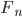
\includegraphics{images/image1.png}{~=
}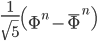
\includegraphics{images/image4.png}

Dove con $\Phi$ si indica la sezione aurea $\frac{1+\sqrt{5}}{2} \simeq -0,618$ e con $\overline{\Phi}$ si indica $\frac{1-\sqrt{5}}{2} \simeq -0,618$

{Dimostrazione}

{Dimostriamo per Induzione la formula di Binet:}

{Base \#1}

{n = 1}

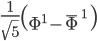
\includegraphics{images/image9.png}

{}

{}

{sostistuisco con le definizioni di $\Phi$ e semplifico}

{= 1 = }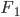
\includegraphics{images/image10.png}

{Base \#2}

{n = 2}

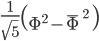
\includegraphics{images/image11.png}

{sostistuisco con le definizioni di $\Phi$ e semplifico}

{= 1 = }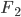
\includegraphics{images/image12.png}

{Passo induttivo}

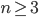
\includegraphics{images/image13.png}

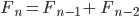
\includegraphics{images/image14.png}{~}

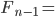
\includegraphics{images/image15.png}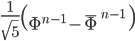
\includegraphics{images/image16.png}{~e
}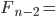
\includegraphics{images/image17.png}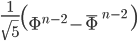
\includegraphics{images/image18.png}

{~}

{}

{assomiglia alla forma }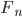
\includegraphics{images/image1.png}{~=
}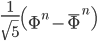
\includegraphics{images/image4.png}{~}

{ci chiediamo se }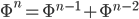
\includegraphics{images/image19.png}{~e se
}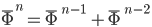
\includegraphics{images/image20.png}

{divido da entrambe le parti per
}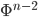
\includegraphics{images/image21.png}{~e
}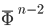
\includegraphics{images/image22.png}

{}

{Definizione \#1}

{}

{Utilizzeremo la notazione }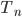
\includegraphics{images/image23.png}{~per
indicare la velocità/complessità di una particolare funzione (numero di
righe di codice eseguite) }

{}

{Fib1 (int n) → int}

{~~~~~~~~return }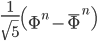
\includegraphics{images/image4.png}

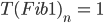
\includegraphics{images/image24.png}{~}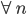
\includegraphics{images/image25.png}

{}

{}

{}

{Problema: con l'aumentare di n, la funzione Fib1(n) diventa sempre più
imprecisa}

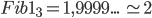
\includegraphics{images/image26.png}

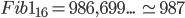
\includegraphics{images/image27.png}

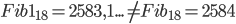
\includegraphics{images/image28.png}

{}

{Definizione \#2}

\protect\hypertarget{t.b6ceb73d86c2dc3f3cbc86e1ad6e301e593880f5}{}{}\protect\hypertarget{t.0}{}{}

\begin{longtable}[]{@{}l@{}}
\toprule
\begin{minipage}[t]{0.97\columnwidth}\raggedright\strut
{Fib2 (}{int}{~n) → }{int}{\\
\hspace*{0.333em}\hspace*{0.333em}\hspace*{0.333em}\hspace*{0.333em}\hspace*{0.333em}\hspace*{0.333em}\hspace*{0.333em}\hspace*{0.333em}}{if}{~n
\textless{}= }{2}{~then }{return}{~}{1}{\\
\hspace*{0.333em}\hspace*{0.333em}\hspace*{0.333em}\hspace*{0.333em}\hspace*{0.333em}\hspace*{0.333em}\hspace*{0.333em}\hspace*{0.333em}}{else}{~}{return}{~Fib2(n}{-1}{)
+ Fib2(n}{-2}{)}\strut
\end{minipage}\tabularnewline
\bottomrule
\end{longtable}

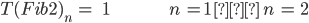
\includegraphics{images/image29.png}

{~~~~~~~~~~~~~~~~}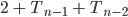
\includegraphics{images/image30.png}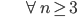
\includegraphics{images/image31.png}

{}

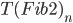
\includegraphics{images/image32.png}{~è una }{formula
ricorsiva}{~}{o}{~}{ricorrenza}

{}

\protect\hypertarget{t.b835927b516aa4a0b07c3acab4f4cd0150ff7dd8}{}{}\protect\hypertarget{t.1}{}{}

\begin{longtable}[]{@{}ll@{}}
\toprule
\begin{minipage}[t]{0.47\columnwidth}\raggedright\strut
{n}\strut
\end{minipage} & \begin{minipage}[t]{0.47\columnwidth}\raggedright\strut
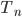
\includegraphics{images/image23.png}{~}\strut
\end{minipage}\tabularnewline
\begin{minipage}[t]{0.47\columnwidth}\raggedright\strut
{1}\strut
\end{minipage} & \begin{minipage}[t]{0.47\columnwidth}\raggedright\strut
{1}\strut
\end{minipage}\tabularnewline
\begin{minipage}[t]{0.47\columnwidth}\raggedright\strut
{2}\strut
\end{minipage} & \begin{minipage}[t]{0.47\columnwidth}\raggedright\strut
{1}\strut
\end{minipage}\tabularnewline
\begin{minipage}[t]{0.47\columnwidth}\raggedright\strut
{3}\strut
\end{minipage} & \begin{minipage}[t]{0.47\columnwidth}\raggedright\strut
{2 + 1 + 1 = 4}\strut
\end{minipage}\tabularnewline
\begin{minipage}[t]{0.47\columnwidth}\raggedright\strut
{4}\strut
\end{minipage} & \begin{minipage}[t]{0.47\columnwidth}\raggedright\strut
{2 + 4 + 1 = 7}\strut
\end{minipage}\tabularnewline
\begin{minipage}[t]{0.47\columnwidth}\raggedright\strut
{5}\strut
\end{minipage} & \begin{minipage}[t]{0.47\columnwidth}\raggedright\strut
{2 + 7 + 4 = 13}\strut
\end{minipage}\tabularnewline
\bottomrule
\end{longtable}

{}

{Risolviamo la ricorrenza per determinare la complessità / bontà della
funzione esaminata.}

\begin{itemize}
\tightlist
\item
  {andamento esponenziale rispetto ad n → funzione NON efficiente}
\item
  {andamento logaritmico / proporzionale rispetto ad n → funzione
  efficiente}
\end{itemize}

{}

{}

{}

{}

\begin{center}\rule{0.5\linewidth}{\linethickness}\end{center}

{}

\hypertarget{h.x4ciu865ga1f}{\subsubsection{\texorpdfstring{{Strumento
\#1 - albero di
ricorsione}}{Strumento \#1 - albero di ricorsione}}\label{h.x4ciu865ga1f}}

{}

{Notiamo che }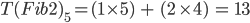
\includegraphics{images/image33.png}

{dove (1 * 5) è la complessità delle foglie (5 foglie con peso 1)}

{e (2 * 4) è la complessità dei nodi interni (4 nodi con peso 2)}

{}

{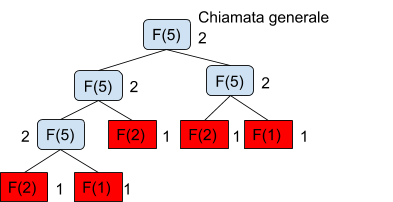
\includegraphics{images/image523.png}}

{Proprietà \#1}

{}

{Se }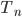
\includegraphics{images/image23.png}{rappresenta l'albero di
ricorsione relativo a }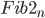
\includegraphics{images/image34.png}{allora il
numero di foglie di }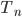
\includegraphics{images/image23.png}{è uguale a
}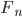
\includegraphics{images/image1.png}{(con
}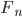
\includegraphics{images/image1.png}{indichiamo l'n-esimo numero della
successione di Fibonacci)}

{}

{Dimostrazione per induzione}

{}

{Base:}

{se n = ~1 → numero di foglie di }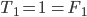
\includegraphics{images/image35.png}

{se n = ~2 → numero di foglie di }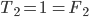
\includegraphics{images/image36.png}

{}

{Passo induttivo:}

{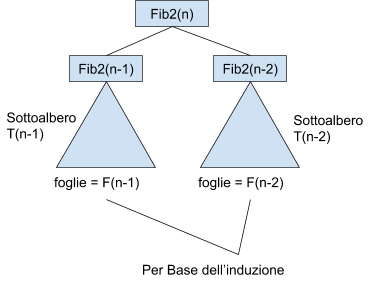
\includegraphics{images/image528.png}}

{~~~~~~~~}

{}

{}

{Proprietà \#2}

{}

{Sia}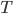
\includegraphics{images/image37.png}{un albero binario in cui ogni
nodo interno ha esattamente 2 figli}

{Allora }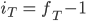
\includegraphics{images/image38.png}

{dove ~~~~~~~~con }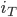
\includegraphics{images/image39.png}{indichiamo il
numero di nodi interni dell'albero }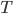
\includegraphics{images/image37.png}

{e con }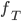
\includegraphics{images/image40.png}{indichiamo il numero di
foglie dell'albero }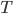
\includegraphics{images/image37.png}

{}

{}

{Dimostrazione per induzione}

{dimostrazione su }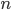
\includegraphics{images/image41.png}{, dove
}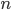
\includegraphics{images/image41.png}{~è il numero di nodi di
}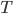
\includegraphics{images/image37.png}

{}

{Base:}

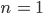
\includegraphics{images/image42.png}{~→ OVVIO}

{}

{Passo induttivo:}

{~~~~~~~~~~~~~~~~}\includegraphics{images/image43.png}

{~~~~~~~~}{\includegraphics{images/image525.png}}

{\includegraphics{images/image536.png}}

{L'albero risultante lo chiamiamo
}\includegraphics{images/image44.png}{~:}

{\includegraphics{images/image522.png}}

{}

{Notiamo che }

\includegraphics{images/image45.png}{*}

{}

\includegraphics{images/image46.png}{**}

\includegraphics{images/image47.png}{~ ~}

{→ (inverto) ~ ~}\includegraphics{images/image48.png}{~ }

{→ (sostituisco }{*}{) }\includegraphics{images/image49.png}

{→ (semplifico) ~}\includegraphics{images/image50.png}{~ }

{→ (sostituisco }{**}{) ~ }\includegraphics{images/image38.png}

{}

{Studio complessità di }\includegraphics{images/image51.png}{l'utilizzo
del metodo dell'albero di ricorsione}

{}

{~}\includegraphics{images/image52.png}

{~}\includegraphics{images/image53.png}

{}

\includegraphics{images/image54.png}

{→ }\includegraphics{images/image55.png}

{→ }\includegraphics{images/image56.png}{~}

{Proprietà \#3}

{}

\includegraphics{images/image57.png}

{Dimostrazione per induzione}

{Base:}

{~~~~~~~~}\includegraphics{images/image58.png}

\includegraphics{images/image59.png}

\includegraphics{images/image60.png}

{Passo induttivo:}

{~~~~~~~~}\includegraphics{images/image61.png}

{}

\includegraphics{images/image62.png}

\includegraphics{images/image63.png}

\includegraphics{images/image64.png}

{}

\includegraphics{images/image65.png}{~è sempre maggiore o uguale ad 1}

{}

{Fib2(n) risulta essere troppo poco efficiente}

\includegraphics{images/image66.png}

\includegraphics{images/image67.png}

{}

{Definiamo allora Fib3(n) utilizzando l'iterazione al posto della
ricorsione}

{}

\protect\hypertarget{t.aae11fb7a2c0b52467b2ae76a760f55e201df9fd}{}{}\protect\hypertarget{t.2}{}{}

\begin{longtable}[]{@{}l@{}}
\toprule
\begin{minipage}[t]{0.97\columnwidth}\raggedright\strut
{Fib3 (int }{n}{) --\textgreater{} int\\
\hspace*{0.333em} ~ }{//Allocazione di un array lungo n;}{\\
\hspace*{0.333em} ~ }{F}{(1) = 1; }{F}{(2) = 1;\\
\hspace*{0.333em} ~ }{For}{~i = 3 to }{n}{~\\
\hspace*{0.333em} ~ ~ ~ }{F}{(i) = }{F}{(i-1) + }{F}{(i-2);\\
\hspace*{0.333em} ~ }{Return}{~}{F}{(}{n}{)}\strut
\end{minipage}\tabularnewline
\bottomrule
\end{longtable}

{}

\includegraphics{images/image68.png}

{}

{Ci chiediamo se fib3 sia efficiente dal punto di vista della
memoria\ldots{}}

\begin{center}\rule{0.5\linewidth}{\linethickness}\end{center}

\section{\texorpdfstring{{}}{}}\label{h.t0xc4p18h6wu}

\hypertarget{h.jkxlloc1lefg}{\section{\texorpdfstring{{Notazione
asintotica: le classi O, Omega, Theta
}}{Notazione asintotica: le classi O, Omega, Theta }}\label{h.jkxlloc1lefg}}

{{[}DFI{]} 2.2; {[}CLRS{]} 3.1}

{}

{}

{}

\hypertarget{h.tn5j57miv2l8}{\section{\texorpdfstring{{Esercizi sulla
notazione asintotica. Le classi o,
omega}}{Esercizi sulla notazione asintotica. Le classi o, omega}}\label{h.tn5j57miv2l8}}

{{[}CLRS{]} 3.1}

{}

{}

\hypertarget{h.qp9ilz1tito1}{\section{\texorpdfstring{{Divide et impera.
Il teorema fondamentale delle ricorrenze (o ``Teorema master'').
Esercizi.}}{Divide et impera. Il teorema fondamentale delle ricorrenze (o Teorema master). Esercizi.}}\label{h.qp9ilz1tito1}}

{{[}DFI{]} 2.5; {[}CLRS{]} 4.3}

{}

{}

{}

\hypertarget{h.a5tr7osf4zwh}{\section{\texorpdfstring{{Rappresentazione
di una lista attraverso un vettore
(matrice)}}{Rappresentazione di una lista attraverso un vettore (matrice)}}\label{h.a5tr7osf4zwh}}

{}

{La lista è doppiamente concatenata, ovvero contiene riferimento sia
all'elemento precedente che a quello successivo.}

{}

{La costante NULL viene rappresentata da un indice che non appartiene
all'insieme degli indici del vettore (0 in pseudocodice, -1 in C)}

{}

{\includegraphics{images/image520.png}}

{}

{}

{Analogamente si può creare una lista singolarmente concatenata chiamata
FreeList contenente le celle libere (i campi Key e Previous si possono
ignorare). Essa verrà utilizzata per l'allocazione di una nuova lista.
FreeList è una variabile globale.}

{}

{All'inizio {[}\ldots{}{]} la FreeList contiene TUTTI gli oggetti non
allocati.}

{}

{Allocate\_Object()~~~~~~~~~~~~~~~~~~~~~~~~~~~~~~~~}{Complessità
}\includegraphics{images/image69.png}

{~~~~~~~~}

\protect\hypertarget{t.6867fb3c644d0c0b07e14f5253c873dd313c05de}{}{}\protect\hypertarget{t.3}{}{}

\begin{longtable}[]{@{}l@{}}
\toprule
\begin{minipage}[t]{0.97\columnwidth}\raggedright\strut
{if}{(}{free}{~== null)\\
\hspace*{0.333em}\hspace*{0.333em}\hspace*{0.333em}\hspace*{0.333em}\hspace*{0.333em}\hspace*{0.333em}\hspace*{0.333em}\hspace*{0.333em}\hspace*{0.333em}\hspace*{0.333em}\hspace*{0.333em}\hspace*{0.333em}\hspace*{0.333em}\hspace*{0.333em}\hspace*{0.333em}\hspace*{0.333em}errore
}{``spazio esaurito''}{\\
\hspace*{0.333em}\hspace*{0.333em}\hspace*{0.333em}\hspace*{0.333em}\hspace*{0.333em}\hspace*{0.333em}\hspace*{0.333em}\hspace*{0.333em}}{else}{\\
\hspace*{0.333em}\hspace*{0.333em}\hspace*{0.333em}\hspace*{0.333em}\hspace*{0.333em}\hspace*{0.333em}\hspace*{0.333em}\hspace*{0.333em}\hspace*{0.333em}\hspace*{0.333em}\hspace*{0.333em}\hspace*{0.333em}\hspace*{0.333em}\hspace*{0.333em}\hspace*{0.333em}\hspace*{0.333em}x
= }{free}{\\
\hspace*{0.333em}\hspace*{0.333em}\hspace*{0.333em}\hspace*{0.333em}\hspace*{0.333em}\hspace*{0.333em}\hspace*{0.333em}\hspace*{0.333em}\hspace*{0.333em}\hspace*{0.333em}\hspace*{0.333em}\hspace*{0.333em}\hspace*{0.333em}\hspace*{0.333em}\hspace*{0.333em}\hspace*{0.333em}}{free}{~=
nexy{[}}{free}{{]}\\
\hspace*{0.333em}\hspace*{0.333em}\hspace*{0.333em}\hspace*{0.333em}\hspace*{0.333em}\hspace*{0.333em}\hspace*{0.333em}\hspace*{0.333em}\hspace*{0.333em}\hspace*{0.333em}\hspace*{0.333em}\hspace*{0.333em}\hspace*{0.333em}\hspace*{0.333em}\hspace*{0.333em}\hspace*{0.333em}}{return}{~x}\strut
\end{minipage}\tabularnewline
\bottomrule
\end{longtable}

{~~~~~~~~~~~~~~~~}

{}

{\#Inserisce la cella da liberare in testa alla FreeList}

{Free\_Object(x)}{~~~~~~~~~~~~~~~~~~~~~~~~~~~~~~~~Complessità
}\includegraphics{images/image69.png}

{~~~~~~~~}

\protect\hypertarget{t.ca6d9bfbccaf8ba905655d1fba7938b11c658c64}{}{}\protect\hypertarget{t.4}{}{}

\begin{longtable}[]{@{}l@{}}
\toprule
\begin{minipage}[t]{0.97\columnwidth}\raggedright\strut
{next{[}x{]} = }{free}{\\
\hspace*{0.333em}\hspace*{0.333em}\hspace*{0.333em}\hspace*{0.333em}\hspace*{0.333em}\hspace*{0.333em}\hspace*{0.333em}\hspace*{0.333em}}{free}{~=
x}\strut
\end{minipage}\tabularnewline
\bottomrule
\end{longtable}

{}

{}

{}

\begin{center}\rule{0.5\linewidth}{\linethickness}\end{center}

\section{\texorpdfstring{{}}{}}\label{h.eidcfonq0wug}

\hypertarget{h.rgokfftftjlb}{\section{\texorpdfstring{{Alberi}}{Alberi}}\label{h.rgokfftftjlb}}

{{[}CLRS{]} pp. 977-979}

{}

{L'albero è un tipo particolare di grafo connesso, aciclico e non
orientato.}

{}

{Un albero radicato è una coppia }\includegraphics{images/image70.png}

\includegraphics{images/image71.png}{~è un insieme finito di nodi fra
cui si distingue un nodo }\includegraphics{images/image72.png}{~detto
`Radice'.}

\includegraphics{images/image73.png}{~è un sottoinsieme del prodotto
cartesiano }\includegraphics{images/image74.png}{,è un insieme di coppie
di nodi che chiamiamo }{archi}{.}

{}

{}

{In un albero, ogni nodo v (eccetto la radice) ha esattamente un
genitore che viene chiamato padre u, tale che
}\includegraphics{images/image75.png}

{\includegraphics{images/image539.png}}

{}

{Un nodo può avere 0 o più figli, un figlio è tale se esiste un arco
}\includegraphics{images/image75.png}

{}

{Il numero dei figli di un nodo si chiama GRADO del nodo.}

{Un nodo senza figli è detto FOGLIA o NODO ESTERNO.}

{Un nodo non foglia è un NODO INTERNO.}

{Se due nodi hanno lo stesso padre, allora sono fratelli.}

{}

{Il cammino da}{~}\includegraphics{images/image76.png}{~ad
}\includegraphics{images/image77.png}{nell'albero
}\includegraphics{images/image37.png}{~è una sequenza di nodi
}\includegraphics{images/image78.png}{tale che soddisfa queste
condizioni:}

{~~~~~~~~}\includegraphics{images/image79.png}

{~~~~~~~~}\includegraphics{images/image80.png}

{~~~~~~~~}\includegraphics{images/image81.png}

{~~~~~~~~}

{La lunghezza di un cammino è il numero di archi nel cammino oppure il
numero di nodi - 1.}

{}

{Sia }\includegraphics{images/image82.png}{~un nodo dell'albero radicato
}\includegraphics{images/image37.png}{con radice
}\includegraphics{images/image83.png}{.}

{Qualsiasi nodo }\includegraphics{images/image84.png}{~in un cammino che
parte dalla radice }\includegraphics{images/image83.png}{~ed arriva ad
}\includegraphics{images/image82.png}{è detto ANTENATO di
}\includegraphics{images/image82.png}{~(}\includegraphics{images/image82.png}{~compreso,
è antenato di se stesso).}

{}

{Se }\includegraphics{images/image84.png}{~è un antenato di
}\includegraphics{images/image82.png}{, allora
}\includegraphics{images/image82.png}{~è DISCENDENTE di
}\includegraphics{images/image84.png}

{}

{NB: Ogni nodo è DISCENDENTE ed ANTENATO di sè stesso.}

{}

{Se }\includegraphics{images/image84.png}{~è un antenato di
}\includegraphics{images/image82.png}{~ed
}\includegraphics{images/image82.png}{~è diverso da
}\includegraphics{images/image84.png}{, allora
}\includegraphics{images/image84.png}{~è un ANTENATO PROPRIO di
}\includegraphics{images/image82.png}{~ed
}\includegraphics{images/image82.png}{~è DISCENDENTE PROPRIO di
}\includegraphics{images/image84.png}{.}

{Il sottoalbero con radice in }\includegraphics{images/image82.png}{~è
l'albero indotto dai discendenti di
}\includegraphics{images/image82.png}

{La profondità}{~di un nodo }\includegraphics{images/image82.png}{~è la
lunghezza del cammino dalla radice ad
}\includegraphics{images/image82.png}{.}

{Un livello di un albero è costituito da tutti i nodi che stanno alla
stessa profondità. }

{L'altezza}{~di un nodo }\includegraphics{images/image82.png}{~è la
lunghezza del più lungo cammino che scende da
}\includegraphics{images/image82.png}{~alle foglie (qualsiasi foglia) di
profondità massima.}

{L'altezza di un albero è l'altezza del nodo radice.}

{L'altezza è la massima profondità di un qualsiasi nodo dell'albero.}

{}

\hypertarget{h.rmzlh8kpnju}{\subsection{\texorpdfstring{{Alberi binari
(Albero k-ario con K =
2)}}{Alberi binari (Albero k-ario con K = 2)}}\label{h.rmzlh8kpnju}}

{}

{Gli alberi binari sono definiti in modo ricorsivo:}

\begin{itemize}
\tightlist
\item
  {Un albero vuoto è binario}
\item
  {Un albero costituito da un nodo (radice) ,}
\end{itemize}

{~~~~~~~~~~~~~~~~da un albero binario detto sottoalbero sinistro della
radice,}

{~~~~~~~~~~~~~~~~e da un'altro albero binario detto sottoalbero destro
della radice}

{~~~~~~~~~~~~~~~~è detto un albero binario.}

{}

\hypertarget{h.chua2o837in5}{\subsection{\texorpdfstring{{Albero
k-ario}}{Albero k-ario}}\label{h.chua2o837in5}}

{E' un albero in cui i figli si un nodo sono etichettati con interi
positivi distinti e le etichette maggiori di
}\includegraphics{images/image85.png}{~sono assenti = ogni nodo può
avere al più }\includegraphics{images/image85.png}{~figli.}

{}

{Un albero K-ario completo è tale quando tutte le foglie hanno la stessa
profondità e tutti i nodi interni hanno grado
}\includegraphics{images/image85.png}{~}

{}

{ALGORITMO}

{Trovare l'algoritmo per determinare la completezza di un albero}

{}

{Dimostro}{~per induzione che le foglie sono
}\includegraphics{images/image86.png}{~}

{}

\includegraphics{images/image87.png}{~(caso base)
}\includegraphics{images/image88.png}{~OK}

{assumiamo che per un albero di altezza
}\includegraphics{images/image89.png}{~sia vero che
}\includegraphics{images/image90.png}

{lo dimostro per }\includegraphics{images/image91.png}

{}

{il numero di nodi di profondità
}\includegraphics{images/image89.png}{~è
}\includegraphics{images/image86.png}{per ipotesi}

{il numero di nodi di profondità
}\includegraphics{images/image91.png}{~è
}\includegraphics{images/image92.png}{~OK}

{}

{ALGORITMO}

{Trovare il numero di foglie e il numero di nodi interni di un albero
k-ario completo di altezza }\includegraphics{images/image89.png}{~}

{}

\includegraphics{images/image93.png}{~è una sommatoria GEOMETRICA, si
semplifica in }\includegraphics{images/image94.png}{, quindi
}\includegraphics{images/image95.png}

{}

{Altezza di un albero k-ario completo con
}\includegraphics{images/image41.png}{~nodi:}

\includegraphics{images/image96.png}{~→
}\includegraphics{images/image97.png}{~→
}\includegraphics{images/image98.png}

{}

{}

{Proprietà}

{Dimostrare per induzione che in un albero BINARIO completo non nullo
avente }\includegraphics{images/image41.png}{nodi, il numero di foglie è
}\includegraphics{images/image99.png}

{}

{}

{}

{}

{}

{}

\hypertarget{h.8kg49eb4dpz1}{\subsubsection{\texorpdfstring{{Tipo di
dato ALBERO}}{Tipo di dato ALBERO}}\label{h.8kg49eb4dpz1}}

{}

{Struttura:}

{}

{Insieme di nodi}

{Insieme di archi}

{}

{Le operazioni del tipo ALBERO:}

{}

{~~~~~~~~newTree() → T~~~~~~~~~~~~~~~~Nuovo albero T}

{~~~~~~~~numNodi(T) → int~~~~~~~~~~~~~~~~Numero di nodi presenti in T}

{~~~~~~~~grado(T,N) → int~~~~~~~~~~~~~~~~Numero di figli di N, N
appartenente a T}

{~~~~~~~~padre(T,N) → int~~~~~~~~~~~~~~~~Nodo padre, null se N è radice,
~N appartenente a T}

{~~~~~~~~figli(T,N) → int{[}{]}~~~~~~~~~~~~~~~~Lista contenente i figli
del nodo N, N appartenente a T}

{}

\hypertarget{h.ueuovjwdu9zj}{\section{\texorpdfstring{{Rappresentazione
di alberi tramite
array}}{Rappresentazione di alberi tramite array}}\label{h.ueuovjwdu9zj}}

{}

\begin{enumerate}
\item ~
  \hypertarget{h.nrzs3ooed9o}{\subsection{\texorpdfstring{{Utilizzo del
  vettore padri}}{Utilizzo del vettore padri}}\label{h.nrzs3ooed9o}}
\end{enumerate}

{}

{}

{}

{}

{sia }\includegraphics{images/image100.png}

{Costruisco un vettore di dimensione
}\includegraphics{images/image41.png}{, le cui celle contengono copie di
}\includegraphics{images/image101.png}{. Con
}\includegraphics{images/image102.png}{~indichiamo l'informazione del
nodo e con }\includegraphics{images/image103.png}{~indichiamo il nodo
padre (indice).}

{}

\includegraphics{images/image104.png}

{p{[}v{]} → info = contenuto}

{p{[}v{]} → padre = indice del padre,
}\includegraphics{images/image105.png}{, se
}\includegraphics{images/image76.png}{~è radice il padre è NULL/-1/0}

{}

{Spazio per memorizzare }\includegraphics{images/image106.png}

{}

\hypertarget{h.ncrwkhkrovb2}{\subsubsection{\texorpdfstring{{Implementazioni:}}{Implementazioni:}}\label{h.ncrwkhkrovb2}}

{Padre - }{Complessità}\includegraphics{images/image107.png}

\protect\hypertarget{t.13d3d44b5647536d159823e4ed75c88728308b7e}{}{}\protect\hypertarget{t.5}{}{}

\begin{longtable}[]{@{}l@{}}
\toprule
\begin{minipage}[t]{0.97\columnwidth}\raggedright\strut
{padre(Tree P, Node v)\\
\hspace*{0.333em}\hspace*{0.333em}\hspace*{0.333em}\hspace*{0.333em}\hspace*{0.333em}\hspace*{0.333em}\hspace*{0.333em}\hspace*{0.333em}}{if}{~(
p{[}v{]} == }{0}{~)\\
\hspace*{0.333em}\hspace*{0.333em}\hspace*{0.333em}\hspace*{0.333em}\hspace*{0.333em}\hspace*{0.333em}\hspace*{0.333em}\hspace*{0.333em}\hspace*{0.333em}\hspace*{0.333em}\hspace*{0.333em}\hspace*{0.333em}\hspace*{0.333em}\hspace*{0.333em}\hspace*{0.333em}\hspace*{0.333em}}{return}{~}{null}{\\
\hspace*{0.333em} ~ ~}{else}{\\
\hspace*{0.333em} ~ ~ ~ ~ ~}{return}{~p{[}v{]} → parent;}\strut
\end{minipage}\tabularnewline
\bottomrule
\end{longtable}

{}

{Figli - }{Complessità }\includegraphics{images/image108.png}

\protect\hypertarget{t.7a531182f90cd5bf7a846292288a5a5bf5dd6eaa}{}{}\protect\hypertarget{t.6}{}{}

\begin{longtable}[]{@{}l@{}}
\toprule
\begin{minipage}[t]{0.97\columnwidth}\raggedright\strut
{figli(Tree P, Node v)\\
\hspace*{0.333em} ~ l = crealista()\\
\hspace*{0.333em} ~ }{for}{~}{i}{~= }{1}{~to n\\
\hspace*{0.333em} ~ ~ ~ ~}{if}{~( p{[}i{]} → parent == v )\\
\hspace*{0.333em}\hspace*{0.333em}\hspace*{0.333em}\hspace*{0.333em}\hspace*{0.333em}\hspace*{0.333em}\hspace*{0.333em}\hspace*{0.333em}
~ ~inserisci(}{i}{,l)\\
\hspace*{0.333em} ~ }{return}{~l}\strut
\end{minipage}\tabularnewline
\begin{minipage}[t]{0.97\columnwidth}\raggedright\strut
{}\strut
\end{minipage}\tabularnewline
\bottomrule
\end{longtable}

{}

{}

{}

\hypertarget{h.5u7fhayyby4r}{\subsection{\texorpdfstring{{2) Utilizzo
del vettore
posizionale}}{2) Utilizzo del vettore posizionale}}\label{h.5u7fhayyby4r}}

{}

{L'albero deve essere completo e con
}\includegraphics{images/image109.png}{. La ricerca è ottimizzata
rispetto all'albero dei padri. Ogni nodo ha una posizione prestabilita.}

{Utilizzo un vettore posizionale P di dimensione n tale che }

\begin{enumerate}
\tightlist
\item
  {0 è la posizione della radice}
\item
  {l'i-esimo figlio di un certo nodo v è in posizione
  }\includegraphics{images/image110.png}{, con
  }\includegraphics{images/image111.png}
\end{enumerate}

{}

{un nodo }\includegraphics{images/image112.png}{~è foglia se non ha
figli, quindi se }\includegraphics{images/image113.png}

{}

{Il padre del nodo }\includegraphics{images/image112.png}{~è in
posizione }{PII}\includegraphics{images/image114.png}{~(parte intera
inferiore) }{ed i figli si trovano tra
}\includegraphics{images/image115.png}{e
}\includegraphics{images/image116.png}

{}

\hypertarget{h.6c4aui6rl05k}{\subsubsection{\texorpdfstring{{Implementazioni:}}{Implementazioni:}}\label{h.6c4aui6rl05k}}

{}

{Padre - }{Complessità}\includegraphics{images/image107.png}

\protect\hypertarget{t.985fc1f36a4403829b157356928a51ed5f0644e7}{}{}\protect\hypertarget{t.7}{}{}

\begin{longtable}[]{@{}l@{}}
\toprule
\begin{minipage}[t]{0.97\columnwidth}\raggedright\strut
{padre(Tree P, Node v)\\
\hspace*{0.333em}\hspace*{0.333em}\hspace*{0.333em}\hspace*{0.333em}\hspace*{0.333em}\hspace*{0.333em}\hspace*{0.333em}\hspace*{0.333em}}{if}{~(
n == }{0}{~)\\
\hspace*{0.333em}\hspace*{0.333em}\hspace*{0.333em}\hspace*{0.333em}\hspace*{0.333em}\hspace*{0.333em}\hspace*{0.333em}\hspace*{0.333em}\hspace*{0.333em}\hspace*{0.333em}\hspace*{0.333em}\hspace*{0.333em}\hspace*{0.333em}\hspace*{0.333em}\hspace*{0.333em}\hspace*{0.333em}}{return}{~}{null}{\\
\hspace*{0.333em} ~ ~}{else}{\\
\hspace*{0.333em} ~ ~ ~ ~
~}{return}{~}{PII}\textsuperscript{\protect\hyperlink{cmnt1}{{[}a{]}}}{{[}(v}{-1}{)
/ K{]}}\strut
\end{minipage}\tabularnewline
\bottomrule
\end{longtable}

{}

{}

{}

{Figli - }{Complessità}\includegraphics{images/image117.png}{, ~con
}\includegraphics{images/image118.png}{~= grado di
}\includegraphics{images/image76.png}{~}

\protect\hypertarget{t.cd7a9ec4a28abd0a2505b50e0d559923d8963c8d}{}{}\protect\hypertarget{t.8}{}{}

\begin{longtable}[]{@{}l@{}}
\toprule
\begin{minipage}[t]{0.97\columnwidth}\raggedright\strut
{figli(Tree P, Node v)\\
\hspace*{0.333em} ~ ~l = crealista()\\
\hspace*{0.333em} ~ ~}{if}{( kv + }{1}{~n)\\
\hspace*{0.333em} ~ ~ ~ ~ }{return}{~l\\
\hspace*{0.333em} ~ ~}{else}{\\
\hspace*{0.333em} ~ ~ ~ ~ }{for}{~i = }{0}{~to k}{-1}{\\
\hspace*{0.333em} ~ ~ ~ ~ ~ ~ ~inserisci(kv + }{1}{~+ i ,l)\\
\hspace*{0.333em}\hspace*{0.333em}\hspace*{0.333em}\hspace*{0.333em}\hspace*{0.333em}\hspace*{0.333em}\hspace*{0.333em}\hspace*{0.333em}
~ ~ }{return}{~l}\strut
\end{minipage}\tabularnewline
\bottomrule
\end{longtable}

{}

\hypertarget{h.bhzctdrna7ur}{\subsection{\texorpdfstring{{3) Utilizzo di
strutture
collegate}}{3) Utilizzo di strutture collegate}}\label{h.bhzctdrna7ur}}

\hypertarget{h.qoohix7mgjib}{\paragraph{\texorpdfstring{{3.a) Parent +
Childs}}{3.a) Parent + Childs}}\label{h.qoohix7mgjib}}

{}

{Ogni nodo è un record con i seguenti campi:}

{~~~~~~~~k : informazione}

{~~~~~~~~p : puntatore al padre}

{~~~~~~~~}

{~~~~~~~~Se il numero di figli è noto}

{}

{~~~~~~~~~~~~~~~~left : puntatore al figlio sinistro}

{~~~~~~~~~~~~~~~~right : puntatore al figlio destro}

{}

{Altrimenti si utilizza una lista di puntatori ai propri figli}

{}

{c {[}{]} : lista di puntatori ai figli~~~~~~~~}

{}

{Se ogni nodo ha grado al più }\includegraphics{images/image118.png}{, è
possibile mantenere in ogni nodo un puntatore a ciascuno dei possibili
}\includegraphics{images/image118.png}{~figli}

{}

{Spazio necessario: }\includegraphics{images/image119.png}{~, se
}\includegraphics{images/image118.png}{~costante allora
}\includegraphics{images/image120.png}

{}

\hypertarget{h.7iunf1nu58vy}{\subsubsection{\texorpdfstring{{Implementazioni:}}{Implementazioni:}}\label{h.7iunf1nu58vy}}

{Padre - }{Complessità }\includegraphics{images/image121.png}

\protect\hypertarget{t.1fda366af82bd8d3dda4418d0091c3a44b3de824}{}{}\protect\hypertarget{t.9}{}{}

\begin{longtable}[]{@{}l@{}}
\toprule
\begin{minipage}[t]{0.97\columnwidth}\raggedright\strut
{padre(Tree P, Node v)\\
\hspace*{0.333em}\hspace*{0.333em}\hspace*{0.333em}\hspace*{0.333em}\hspace*{0.333em}\hspace*{0.333em}\hspace*{0.333em}\hspace*{0.333em}}{return}{~v
→ p}\strut
\end{minipage}\tabularnewline
\bottomrule
\end{longtable}

{}

{Figli - }{Complessità}\includegraphics{images/image122.png}{, con
}\includegraphics{images/image118.png}{~= grado di
}\includegraphics{images/image76.png}{~ }

{Con k non noto si utilizza un ciclo che scorre c{[}{]}}

\protect\hypertarget{t.124118a94a4960d4f86078198fd0f2c89105856f}{}{}\protect\hypertarget{t.10}{}{}

\begin{longtable}[]{@{}l@{}}
\toprule
\begin{minipage}[t]{0.97\columnwidth}\raggedright\strut
{figli(}{Tree}{~}{P}{, }{Node}{~v)\\
\hspace*{0.333em} ~ l = crealista()\\
\hspace*{0.333em} ~ }{if}{( v → }{left}{~\textless{}\textgreater{}null
)\\
\hspace*{0.333em} ~ ~ ~ ~ inserisci(v → }{left}{~,l)\\
\hspace*{0.333em} ~ }{if}{( v → }{right}{\textless{}\textgreater{}null
)\\
\hspace*{0.333em} ~ ~ ~ ~ inserisci(v → }{right}{,l)\\
\hspace*{0.333em} ~ }{return}{~l}\strut
\end{minipage}\tabularnewline
\bottomrule
\end{longtable}

{}

\hypertarget{h.jlqu76iomg9e}{\paragraph{\texorpdfstring{{3.b) Parent +
Left child + Right
sibling}}{3.b) Parent + Left child + Right sibling}}\label{h.jlqu76iomg9e}}

\paragraph{\texorpdfstring{{}}{}}\label{h.jlqu76iomg9e-1}

{}

{}

{}

{}

{}

{Ogni nodo è un record con i seguenti campi:}

{~~~~~~~~k : informazione}

{~~~~~~~~p : puntatore al padre}

{~~~~~~~~left\_child : puntatore al figlio sinistro}

{~~~~~~~~right\_sibling : puntatore al fratello immediatamente a destra}

{}

\hypertarget{h.ekfyi4oujqjt}{\subsubsection{\texorpdfstring{{Implementazioni:}}{Implementazioni:}}\label{h.ekfyi4oujqjt}}

{Padre - }{Complessità}\includegraphics{images/image107.png}

{}

\protect\hypertarget{t.1fda366af82bd8d3dda4418d0091c3a44b3de824}{}{}\protect\hypertarget{t.11}{}{}

\begin{longtable}[]{@{}l@{}}
\toprule
\begin{minipage}[t]{0.97\columnwidth}\raggedright\strut
{padre(Tree P, Node v)\\
\hspace*{0.333em}\hspace*{0.333em}\hspace*{0.333em}\hspace*{0.333em}\hspace*{0.333em}\hspace*{0.333em}\hspace*{0.333em}\hspace*{0.333em}}{return}{~v
→ p}\strut
\end{minipage}\tabularnewline
\bottomrule
\end{longtable}

{}

{Figli - }{Complessità}\includegraphics{images/image117.png}{~con
}\includegraphics{images/image118.png}{~= grado di
}\includegraphics{images/image76.png}{~ }

{}

\protect\hypertarget{t.3d98f2c9e8b44fd4f200b41e25c7a6ffdbeba100}{}{}\protect\hypertarget{t.12}{}{}

\begin{longtable}[]{@{}l@{}}
\toprule
\begin{minipage}[t]{0.97\columnwidth}\raggedright\strut
{figli(Tree P, Node v)\\
\hspace*{0.333em} ~ l = crealista()\\
\hspace*{0.333em} ~ iter = v → left\_child\\
\hspace*{0.333em} ~ }{while}{~( iter \textless{}\textgreater{}
}{null}{)\\
\hspace*{0.333em}\hspace*{0.333em}\hspace*{0.333em}\hspace*{0.333em}\hspace*{0.333em}\hspace*{0.333em}\hspace*{0.333em}\hspace*{0.333em}
~ ~ inserisci(iter,l)\\
\hspace*{0.333em} ~ ~ ~ ~ iter = iter → right\_sibling\\
\hspace*{0.333em} ~ }{return}{~l ~}\strut
\end{minipage}\tabularnewline
\bottomrule
\end{longtable}

\begin{center}\rule{0.5\linewidth}{\linethickness}\end{center}

\section{\texorpdfstring{{}}{}}\label{h.d2exy8bjqfbs}

\hypertarget{h.ike679k4smgg}{\section{\texorpdfstring{{Algoritmi Di
Visita Degli
Alberi}}{Algoritmi Di Visita Degli Alberi}}\label{h.ike679k4smgg}}

{{[}DFI{]} pp. 77-80}

\hypertarget{h.dvc71mavuqx7}{\subsubsection{\texorpdfstring{{Visita
generica}}{Visita generica}}\label{h.dvc71mavuqx7}}

{}

\protect\hypertarget{t.3fc5afa232d0d5009ba66fff59b11fc6057a782f}{}{}\protect\hypertarget{t.13}{}{}

\begin{longtable}[]{@{}l@{}}
\toprule
\begin{minipage}[t]{0.97\columnwidth}\raggedright\strut
{VisitaGenerica(Node v)\\
\hspace*{0.333em}\hspace*{0.333em}\hspace*{0.333em}\hspace*{0.333em}\hspace*{0.333em}\hspace*{0.333em}\hspace*{0.333em}\hspace*{0.333em}s
= \{ v \}\\
\hspace*{0.333em}\hspace*{0.333em}\hspace*{0.333em}\hspace*{0.333em}\hspace*{0.333em}\hspace*{0.333em}\hspace*{0.333em}\hspace*{0.333em}}{while}{~(
s \textless{}\textgreater{} \{\} )\\
\hspace*{0.333em}\hspace*{0.333em}\hspace*{0.333em}\hspace*{0.333em}\hspace*{0.333em}\hspace*{0.333em}\hspace*{0.333em}\hspace*{0.333em}\hspace*{0.333em}\hspace*{0.333em}\hspace*{0.333em}\hspace*{0.333em}\hspace*{0.333em}\hspace*{0.333em}\hspace*{0.333em}\hspace*{0.333em}u
= }{pop}{(s)\\
\hspace*{0.333em}\hspace*{0.333em}\hspace*{0.333em}\hspace*{0.333em}\hspace*{0.333em}\hspace*{0.333em}\hspace*{0.333em}\hspace*{0.333em}\hspace*{0.333em}\hspace*{0.333em}\hspace*{0.333em}\hspace*{0.333em}\hspace*{0.333em}\hspace*{0.333em}\hspace*{0.333em}\hspace*{0.333em}figli
= VisitaGenerica(u)\\
\hspace*{0.333em}\hspace*{0.333em}\hspace*{0.333em}\hspace*{0.333em}\hspace*{0.333em}\hspace*{0.333em}\hspace*{0.333em}\hspace*{0.333em}\hspace*{0.333em}\hspace*{0.333em}\hspace*{0.333em}\hspace*{0.333em}\hspace*{0.333em}\hspace*{0.333em}\hspace*{0.333em}\hspace*{0.333em}s
= s U figli\\
\hspace*{0.333em}\hspace*{0.333em}\hspace*{0.333em}\hspace*{0.333em}\hspace*{0.333em}\hspace*{0.333em}\hspace*{0.333em}\hspace*{0.333em}}{return}{~s}\strut
\end{minipage}\tabularnewline
\bottomrule
\end{longtable}

{}

{Dimostrare che ha costo
LINEARE}\textsuperscript{\protect\hyperlink{cmnt2}{{[}b{]}}}

{}

\hypertarget{h.6xasx7f8zgn1}{\paragraph{\texorpdfstring{{Teorema}}{Teorema}}\label{h.6xasx7f8zgn1}}

{L'algoritmo di visita, applicato alla radice di un albero con m nodi,
termina in O(m) iterazioni. Lo spazio usato è O (}{n}{)}

{}

\hypertarget{h.zdc8liauzt1c}{\paragraph{\texorpdfstring{{Dimostrazione}}{Dimostrazione}}\label{h.zdc8liauzt1c}}

{Hp: L'inserimento e la cancellazione da S sono effettuati in tempo
costante}

{}

{Ogni nodo verrà inserito ed estratto dall'insieme s una sola volta,
perchè in un albero non si può tornare ad un nodo a partire dai suoi
figli.}

{}

{Quindi le iterazioni del ciclo while saranno al più O(n)}

{Poiché ogno nodo compare al più una volta in S, lo spazio richiesto non
è più alto di O(n)}

{}

\hypertarget{h.5u7m241wpdag}{\subsubsection{\texorpdfstring{{Visita DFS
- Depth first search - Ricerca in
profondità}}{Visita DFS - Depth first search - Ricerca in profondità}}\label{h.5u7m241wpdag}}

{}

{Seguiamo tutti i figli sinistri, andando in profondità fino a che non
si raggiunge la prima foglia sinistra. Solo quando il sottoalbero sx è
stato completamente visitato, si passa ~a visitare il sottoalbero dx}

{}

\protect\hypertarget{t.e3f356e73d933eb65b1a6a8cfd4ee1a50561f73c}{}{}\protect\hypertarget{t.14}{}{}

\begin{longtable}[]{@{}l@{}}
\toprule
\begin{minipage}[t]{0.97\columnwidth}\raggedright\strut
{Dfs\_Visit(Node r)\\
\hspace*{0.333em}\hspace*{0.333em}\hspace*{0.333em}\hspace*{0.333em}\hspace*{0.333em}\hspace*{0.333em}\hspace*{0.333em}\hspace*{0.333em}s
= stack()\\
\hspace*{0.333em}\hspace*{0.333em}\hspace*{0.333em}\hspace*{0.333em}\hspace*{0.333em}\hspace*{0.333em}\hspace*{0.333em}\hspace*{0.333em}}{push}{~(r,s)\\
\hspace*{0.333em}\hspace*{0.333em}\hspace*{0.333em}\hspace*{0.333em}\hspace*{0.333em}\hspace*{0.333em}\hspace*{0.333em}\hspace*{0.333em}}{while}{(not
stackempty(s))\\
\hspace*{0.333em}\hspace*{0.333em}\hspace*{0.333em}\hspace*{0.333em}\hspace*{0.333em}\hspace*{0.333em}\hspace*{0.333em}\hspace*{0.333em}\hspace*{0.333em}\hspace*{0.333em}\hspace*{0.333em}\hspace*{0.333em}\hspace*{0.333em}\hspace*{0.333em}\hspace*{0.333em}\hspace*{0.333em}u
= }{pop}{(s)\\
\hspace*{0.333em}\hspace*{0.333em}\hspace*{0.333em}\hspace*{0.333em}\hspace*{0.333em}\hspace*{0.333em}\hspace*{0.333em}\hspace*{0.333em}\hspace*{0.333em}\hspace*{0.333em}\hspace*{0.333em}\hspace*{0.333em}\hspace*{0.333em}\hspace*{0.333em}\hspace*{0.333em}\hspace*{0.333em}}{if}{(u
\textless{}\textgreater{} }{null}{)\\
\hspace*{0.333em}\hspace*{0.333em}\hspace*{0.333em}\hspace*{0.333em}\hspace*{0.333em}\hspace*{0.333em}\hspace*{0.333em}\hspace*{0.333em}\hspace*{0.333em}\hspace*{0.333em}\hspace*{0.333em}\hspace*{0.333em}\hspace*{0.333em}\hspace*{0.333em}\hspace*{0.333em}\hspace*{0.333em}\hspace*{0.333em}\hspace*{0.333em}\hspace*{0.333em}\hspace*{0.333em}\hspace*{0.333em}\hspace*{0.333em}\hspace*{0.333em}\hspace*{0.333em}Dfs\_Visit(u)\\
\hspace*{0.333em}\hspace*{0.333em}\hspace*{0.333em}\hspace*{0.333em}\hspace*{0.333em}\hspace*{0.333em}\hspace*{0.333em}\hspace*{0.333em}\hspace*{0.333em}\hspace*{0.333em}\hspace*{0.333em}\hspace*{0.333em}\hspace*{0.333em}\hspace*{0.333em}\hspace*{0.333em}\hspace*{0.333em}\hspace*{0.333em}\hspace*{0.333em}\hspace*{0.333em}\hspace*{0.333em}\hspace*{0.333em}\hspace*{0.333em}\hspace*{0.333em}\hspace*{0.333em}}{push}{(u
→ right, s)\\
\hspace*{0.333em}\hspace*{0.333em}\hspace*{0.333em}\hspace*{0.333em}\hspace*{0.333em}\hspace*{0.333em}\hspace*{0.333em}\hspace*{0.333em}\hspace*{0.333em}\hspace*{0.333em}\hspace*{0.333em}\hspace*{0.333em}\hspace*{0.333em}\hspace*{0.333em}\hspace*{0.333em}\hspace*{0.333em}\hspace*{0.333em}\hspace*{0.333em}\hspace*{0.333em}\hspace*{0.333em}\hspace*{0.333em}\hspace*{0.333em}\hspace*{0.333em}\hspace*{0.333em}}{push}{(u
→ left , s)\\
\hspace*{0.333em}\hspace*{0.333em}\hspace*{0.333em}\hspace*{0.333em}\hspace*{0.333em}\hspace*{0.333em}\hspace*{0.333em}\hspace*{0.333em}}{return}{~s}\strut
\end{minipage}\tabularnewline
\bottomrule
\end{longtable}

{}

\hypertarget{h.j29c1mxwyzyn}{\subsubsection{\texorpdfstring{{Visita BFS
- Breadth first search - Ricerca in
ampiezza}}{Visita BFS - Breadth first search - Ricerca in ampiezza}}\label{h.j29c1mxwyzyn}}

{}

\begin{center}\rule{0.5\linewidth}{\linethickness}\end{center}

\section{\texorpdfstring{{}}{}}\label{h.5ptbhdwvisbf}

\hypertarget{h.8cvon0yw5yug}{\section{\texorpdfstring{{Heap}}{Heap}}\label{h.8cvon0yw5yug}}

{Heap: albero quasi completo con tutti i nodi dell'ultimo livello a
sinistra}

{}

{MaxHeap: La radice ha valore maggiore o uguale a quello dei figli}

{MinHeap: La radice ha valore minore o uguale a quello dei figli}

{}

\hypertarget{h.twk46x6owxrr}{\subsubsection{\texorpdfstring{{Lemma
2:}}{Lemma 2:}}\label{h.twk46x6owxrr}}

{Nell'array che rappresenta un heap di }{n}{~elementi, le foglie sono i
nodi con indici che vanno alle posizioni}

{}

\includegraphics{images/image123.png}

{}

{\includegraphics{images/image526.png}}

{}

\protect\hypertarget{t.0db836340677fe77e6dcdbae821987d7a7a9aed8}{}{}\protect\hypertarget{t.15}{}{}

{Elemento}

{16}

{15}

{10}

{14}

{7}

{9}

{3}

{2}

{8}

{1}

{Posizione}

{1°}

{2°}

{3°}

{4°}

{5°}

{6°}

{7°}

{8°}

{9°}

{10°}

{}

{}

{}

{}

\includegraphics{images/image124.png}

\includegraphics{images/image125.png}

\includegraphics{images/image126.png}

\includegraphics{images/image127.png}

\includegraphics{images/image128.png}

{n}

{}

\hypertarget{h.wlc8yrs7inpk}{\subsubsection{\texorpdfstring{{Lemma
3:}}{Lemma 3:}}\label{h.wlc8yrs7inpk}}

{}

{Il teorema definisce la numerosità di nodi con una certa altezza:}

{Ci sono al massimo}\includegraphics{images/image129.png}{nodi di
}{altezza}\textsuperscript{\protect\hyperlink{cmnt3}{{[}c{]}}}{~}{h}{~in
un qualsiasi heap di }{n}{~elementi}

\hypertarget{h.t1rcecigqmbx}{\subsubsection{\texorpdfstring{{Max\_heapify}}{Max\_heapify}}\label{h.t1rcecigqmbx}}

{L'operazione max\_heapify permette di mantenere le proprietà di
maxheap}

{}

{Precondizioni}{:}

{Gli alberi binari con radice in left(i) e right(i) sono maxheap}

{Postcondizioni}{:}

{~~~~~~~~L'albero radicato in i è un maxheap}

{}

\protect\hypertarget{t.cd7cd87746d5c02a44eb80c0828166b19e38f945}{}{}\protect\hypertarget{t.16}{}{}

\begin{longtable}[]{@{}l@{}}
\toprule
\begin{minipage}[t]{0.97\columnwidth}\raggedright\strut
{Max\_heapify( Heap A, Node }{i}{)\\
\hspace*{0.333em}\hspace*{0.333em}\hspace*{0.333em}\hspace*{0.333em}\hspace*{0.333em}\hspace*{0.333em}\hspace*{0.333em}\hspace*{0.333em}l
= left(}{i}{)\\
\hspace*{0.333em}\hspace*{0.333em}\hspace*{0.333em}\hspace*{0.333em}\hspace*{0.333em}\hspace*{0.333em}\hspace*{0.333em}\hspace*{0.333em}r
= right(}{i}{)\\
\hspace*{0.333em}\hspace*{0.333em}\hspace*{0.333em}\hspace*{0.333em}\hspace*{0.333em}\hspace*{0.333em}\hspace*{0.333em}\hspace*{0.333em}}{if}{~(
l \textless{}= A.heapsize AND A{[}l{]} \textgreater{} A{[}i{]} )\\
\hspace*{0.333em}\hspace*{0.333em}\hspace*{0.333em}\hspace*{0.333em}\hspace*{0.333em}\hspace*{0.333em}\hspace*{0.333em}\hspace*{0.333em}\hspace*{0.333em}\hspace*{0.333em}\hspace*{0.333em}\hspace*{0.333em}\hspace*{0.333em}\hspace*{0.333em}\hspace*{0.333em}\hspace*{0.333em}massimo
= l\\
\hspace*{0.333em}\hspace*{0.333em}\hspace*{0.333em}\hspace*{0.333em}\hspace*{0.333em}\hspace*{0.333em}\hspace*{0.333em}\hspace*{0.333em}}{else}{\\
\hspace*{0.333em}\hspace*{0.333em}\hspace*{0.333em}\hspace*{0.333em}\hspace*{0.333em}\hspace*{0.333em}\hspace*{0.333em}\hspace*{0.333em}\hspace*{0.333em}\hspace*{0.333em}\hspace*{0.333em}\hspace*{0.333em}\hspace*{0.333em}\hspace*{0.333em}\hspace*{0.333em}\hspace*{0.333em}massimo
=
}{i}{\\[2\baselineskip]\hspace*{0.333em}\hspace*{0.333em}\hspace*{0.333em}\hspace*{0.333em}\hspace*{0.333em}\hspace*{0.333em}\hspace*{0.333em}\hspace*{0.333em}}{if}{~(
r \textless{}= A.heapsize AND A{[}r{]} \textgreater{} A{[}massimo{]} )\\
\hspace*{0.333em}\hspace*{0.333em}\hspace*{0.333em}\hspace*{0.333em}\hspace*{0.333em}\hspace*{0.333em}\hspace*{0.333em}\hspace*{0.333em}\hspace*{0.333em}\hspace*{0.333em}\hspace*{0.333em}\hspace*{0.333em}\hspace*{0.333em}\hspace*{0.333em}\hspace*{0.333em}\hspace*{0.333em}massimo
=
r\\[2\baselineskip]\hspace*{0.333em}\hspace*{0.333em}\hspace*{0.333em}\hspace*{0.333em}\hspace*{0.333em}\hspace*{0.333em}\hspace*{0.333em}\hspace*{0.333em}}{if}{~(
massimo != }{i}{~)\\
\hspace*{0.333em}\hspace*{0.333em}\hspace*{0.333em}\hspace*{0.333em}\hspace*{0.333em}\hspace*{0.333em}\hspace*{0.333em}\hspace*{0.333em}\hspace*{0.333em}\hspace*{0.333em}\hspace*{0.333em}\hspace*{0.333em}\hspace*{0.333em}\hspace*{0.333em}\hspace*{0.333em}\hspace*{0.333em}scambia
( A{[}i{]} , A{[}massimo{]} )\\
\hspace*{0.333em}\hspace*{0.333em}\hspace*{0.333em}\hspace*{0.333em}\hspace*{0.333em}\hspace*{0.333em}\hspace*{0.333em}\hspace*{0.333em}\hspace*{0.333em}\hspace*{0.333em}\hspace*{0.333em}\hspace*{0.333em}\hspace*{0.333em}\hspace*{0.333em}\hspace*{0.333em}\hspace*{0.333em}}{max\_heapify}\textsuperscript{\protect\hyperlink{cmnt4}{{[}d{]}}}{(A,
massimo)}\strut
\end{minipage}\tabularnewline
\bottomrule
\end{longtable}

{}

{Tempo di esecuzione : O(h) dove h è l'altezza del nodi i poichè l'heap
ha altezza log(n) (LEMMA 2)}

{}

\hypertarget{h.symae1e4ut5b}{\subsection{\texorpdfstring{{Dato un
vettore disordinato, costruire un
heap}}{Dato un vettore disordinato, costruire un heap}}\label{h.symae1e4ut5b}}

{}

\protect\hypertarget{t.7cd7f95f2cb15308ae008ffe6fd7598b3dd68d3c}{}{}\protect\hypertarget{t.17}{}{}

\begin{longtable}[]{@{}l@{}}
\toprule
\begin{minipage}[t]{0.97\columnwidth}\raggedright\strut
{Build\_maxheap ( Array A )\\
\hspace*{0.333em}\hspace*{0.333em}\hspace*{0.333em}\hspace*{0.333em}\hspace*{0.333em}\hspace*{0.333em}\hspace*{0.333em}\hspace*{0.333em}A.heapsize
= A.}{length}{\\
\hspace*{0.333em}\hspace*{0.333em}\hspace*{0.333em}\hspace*{0.333em}\hspace*{0.333em}\hspace*{0.333em}\hspace*{0.333em}\hspace*{0.333em}}{for}{~}{i}{~in
}{PII}\textsuperscript{\protect\hyperlink{cmnt5}{{[}e{]}}}{~(
A.}{length}{~/ }{2}{~) downto }{1}{\\
\hspace*{0.333em}\hspace*{0.333em}\hspace*{0.333em}\hspace*{0.333em}\hspace*{0.333em}\hspace*{0.333em}\hspace*{0.333em}\hspace*{0.333em}\hspace*{0.333em}\hspace*{0.333em}\hspace*{0.333em}\hspace*{0.333em}\hspace*{0.333em}\hspace*{0.333em}\hspace*{0.333em}\hspace*{0.333em}max\_heapify
( A , }{i}{~)}\strut
\end{minipage}\tabularnewline
\bottomrule
\end{longtable}

{}

{Invariante: ogni nodo in posizione
}\includegraphics{images/image130.png}{~è radice di un maxheap, }{con n
= }

{}

{Sembrerebbe complessa }\includegraphics{images/image131.png}{ma
max\_heapify lavora principalmente su foglie, }{quindi la complessità è
lineare }\includegraphics{images/image132.png}{.}

{}

{}

\includegraphics{images/image133.png}

{L'ultima sommatoria è la serie
nota}\includegraphics{images/image134.png}

{Con }\includegraphics{images/image135.png}{,
}\includegraphics{images/image136.png}

{Quindi }\includegraphics{images/image137.png}

\hypertarget{h.vi4eu8p6i55e}{\subsection{\texorpdfstring{{Heapsort}}{Heapsort}}\label{h.vi4eu8p6i55e}}

\protect\hypertarget{t.6067bda8a5da2e84ade010bd50161a2ed3d5c2cd}{}{}\protect\hypertarget{t.18}{}{}

\begin{longtable}[]{@{}l@{}}
\toprule
\begin{minipage}[t]{0.97\columnwidth}\raggedright\strut
{HeapSort ( Array A )\\
\hspace*{0.333em}\hspace*{0.333em}\hspace*{0.333em}\hspace*{0.333em}\hspace*{0.333em}\hspace*{0.333em}\hspace*{0.333em}\hspace*{0.333em}build\_maxheap
( A )\\
\hspace*{0.333em}\hspace*{0.333em}\hspace*{0.333em}\hspace*{0.333em}\hspace*{0.333em}\hspace*{0.333em}\hspace*{0.333em}\hspace*{0.333em}}{for}{~}{i}{~=
A.}{length}{~downto }{2}{\\
\hspace*{0.333em}\hspace*{0.333em}\hspace*{0.333em}\hspace*{0.333em}\hspace*{0.333em}\hspace*{0.333em}\hspace*{0.333em}\hspace*{0.333em}\hspace*{0.333em}\hspace*{0.333em}\hspace*{0.333em}\hspace*{0.333em}\hspace*{0.333em}\hspace*{0.333em}\hspace*{0.333em}\hspace*{0.333em}scambia
A{[} }{1}{~{]} e A{[} i {]}\\
\hspace*{0.333em}\hspace*{0.333em}\hspace*{0.333em}\hspace*{0.333em}\hspace*{0.333em}\hspace*{0.333em}\hspace*{0.333em}\hspace*{0.333em}\hspace*{0.333em}\hspace*{0.333em}\hspace*{0.333em}\hspace*{0.333em}\hspace*{0.333em}\hspace*{0.333em}\hspace*{0.333em}\hspace*{0.333em}A.heapsize
-= }{1}{\\
\hspace*{0.333em}\hspace*{0.333em}\hspace*{0.333em}\hspace*{0.333em}\hspace*{0.333em}\hspace*{0.333em}\hspace*{0.333em}\hspace*{0.333em}\hspace*{0.333em}\hspace*{0.333em}\hspace*{0.333em}\hspace*{0.333em}\hspace*{0.333em}\hspace*{0.333em}\hspace*{0.333em}\hspace*{0.333em}max\_heapify
( A , }{1}{~)}\strut
\end{minipage}\tabularnewline
\bottomrule
\end{longtable}

{}

{INV = Il sottoarray che va dalla posizione 1 alla posizione i è un
maxheap che contiene gli elementi più piccoli del intero vettore di
partenza, mentre }\includegraphics{images/image138.png}{contiene gli
}\includegraphics{images/image139.png}{~elementi più grandi di
}\includegraphics{images/image140.png}{~}{ordinati}{.}

\hypertarget{h.rdu8s741ww8w}{\subsubsection{\texorpdfstring{{Teorema}}{Teorema}}\label{h.rdu8s741ww8w}}

{L'algoritmo HeapSort ordina }{in loco}{~n elementi eseguendo nel
peggiore dei casi }\includegraphics{images/image141.png}{~confronti in
quanto algoritmo }{basato sui confronti}{.}

{}

\hypertarget{h.jih9riph7gns}{\subsection{\texorpdfstring{{Code di
priorità}}{Code di priorità}}\label{h.jih9riph7gns}}

{{[}CLRS{]} pp. 135-140}

{}

{Struttura dati che serve a mantenere un insieme dinamico i cui elementi
( aggiungibili e rimovibili ) hanno un valore associato detto }{chiave o
peso.}

{}

{Esistono due tipi di code di priorità:}

\begin{itemize}
\tightlist
\item
  {MaxPriorità (Si utilizza la struttura MaxHeap)}
\item
  {MinPriorità (Si utilizza la struttura MinHeap)}
\end{itemize}

{}

{Le operazioni delle code di priorità massima/minima sono:}

{}

{Insert( Coda s , Elemento X)}

{Inserisce l'elemento X in S}

{}

{Maximum( Coda s )}

{Restituisce l'elemento di S con la chiave maggiore senza rimuoverlo}

{}

{Minimum( Coda s) }

{Restituisce l'elemento di S con la chiave minore senza rimuoverlo}

{}

{Extract\_max( Coda s)}

{Elimina e restituisce l'elemento di S con la chiave maggiore}

{}

{Extract\_min( Coda s) }

{Elimina e restituisce l'elemento di S con la chiave minore}

{}

{Increase\_key( Coda s, Elemento x, Chiave k) }

{Incrementa il valore della chiave di X al nuovo valore K. Si suppone
che K sia maggiore o uguale al valore corrente della chiave di X}

\includegraphics{images/image142.png}

{}

{Decrease\_key( Coda s, Elemento x, Chiave k)}

{Decrementa il valore della chiave di X al nuovo valore K. Si suppone
che K sia minore o uguale al valore corrente della chiave di X}

\includegraphics{images/image143.png}

{}

\begin{center}\rule{0.5\linewidth}{\linethickness}\end{center}

\subsection{\texorpdfstring{{}}{}}\label{h.7vrdkvwj5vt}

\hypertarget{h.aocay3iqens1}{\subsection{\texorpdfstring{{Implementazione
di code di massima priorità con le strutture
Heap}}{Implementazione di code di massima priorità con le strutture Heap}}\label{h.aocay3iqens1}}

{}

\protect\hypertarget{t.fb709a8e208067c1bfab491f087053eba0be66c5}{}{}\protect\hypertarget{t.19}{}{}

\begin{longtable}[]{@{}l@{}}
\toprule
\begin{minipage}[t]{0.97\columnwidth}\raggedright\strut
{Heap\_maximum(Heap A)\\
\hspace*{0.333em}\hspace*{0.333em}\hspace*{0.333em}\hspace*{0.333em}\hspace*{0.333em}\hspace*{0.333em}\hspace*{0.333em}\hspace*{0.333em}}{if}{~(
A.heapSize \textless{} }{1}{~)\\
\hspace*{0.333em}\hspace*{0.333em}\hspace*{0.333em}\hspace*{0.333em}\hspace*{0.333em}\hspace*{0.333em}\hspace*{0.333em}\hspace*{0.333em}\hspace*{0.333em}\hspace*{0.333em}\hspace*{0.333em}\hspace*{0.333em}\hspace*{0.333em}\hspace*{0.333em}\hspace*{0.333em}\hspace*{0.333em}}{error}{~}{``heap
underflow''}{\\
\hspace*{0.333em}\hspace*{0.333em}\hspace*{0.333em}\hspace*{0.333em}\hspace*{0.333em}\hspace*{0.333em}\hspace*{0.333em}\hspace*{0.333em}}{else}{\\
\hspace*{0.333em}\hspace*{0.333em}\hspace*{0.333em}\hspace*{0.333em}\hspace*{0.333em}\hspace*{0.333em}\hspace*{0.333em}\hspace*{0.333em}\hspace*{0.333em}\hspace*{0.333em}\hspace*{0.333em}\hspace*{0.333em}\hspace*{0.333em}\hspace*{0.333em}\hspace*{0.333em}\hspace*{0.333em}}{max}{~=
A{[}}{1}{{]}\\
\hspace*{0.333em}\hspace*{0.333em}\hspace*{0.333em}\hspace*{0.333em}\hspace*{0.333em}\hspace*{0.333em}\hspace*{0.333em}\hspace*{0.333em}\hspace*{0.333em}\hspace*{0.333em}\hspace*{0.333em}\hspace*{0.333em}\hspace*{0.333em}\hspace*{0.333em}\hspace*{0.333em}\hspace*{0.333em}}{return}{~}{max}\strut
\end{minipage}\tabularnewline
\bottomrule
\end{longtable}

{Complessità di Heap Maximum : }\includegraphics{images/image121.png}

{}

\protect\hypertarget{t.a2df3fbad46ddea60bea6624e0f6ba11a8bfb6c9}{}{}\protect\hypertarget{t.20}{}{}

\begin{longtable}[]{@{}l@{}}
\toprule
\begin{minipage}[t]{0.97\columnwidth}\raggedright\strut
{Heap\_extract\_max(Heap A)\\
\hspace*{0.333em}\hspace*{0.333em}\hspace*{0.333em}\hspace*{0.333em}\hspace*{0.333em}\hspace*{0.333em}\hspace*{0.333em}\hspace*{0.333em}}{if}{~(
A.heapSize \textless{} }{1}{~)\\
\hspace*{0.333em}\hspace*{0.333em}\hspace*{0.333em}\hspace*{0.333em}\hspace*{0.333em}\hspace*{0.333em}\hspace*{0.333em}\hspace*{0.333em}\hspace*{0.333em}\hspace*{0.333em}\hspace*{0.333em}\hspace*{0.333em}\hspace*{0.333em}\hspace*{0.333em}\hspace*{0.333em}\hspace*{0.333em}}{error}{~}{``heap
underflow''}{\\
\hspace*{0.333em}\hspace*{0.333em}\hspace*{0.333em}\hspace*{0.333em}\hspace*{0.333em}\hspace*{0.333em}\hspace*{0.333em}\hspace*{0.333em}}{else}{\\
\hspace*{0.333em}\hspace*{0.333em}\hspace*{0.333em}\hspace*{0.333em}\hspace*{0.333em}\hspace*{0.333em}\hspace*{0.333em}\hspace*{0.333em}\hspace*{0.333em}\hspace*{0.333em}\hspace*{0.333em}\hspace*{0.333em}\hspace*{0.333em}\hspace*{0.333em}\hspace*{0.333em}\hspace*{0.333em}}{max}{~=
A{[}}{1}{{]}\\
\hspace*{0.333em}\hspace*{0.333em}\hspace*{0.333em}\hspace*{0.333em}\hspace*{0.333em}\hspace*{0.333em}\hspace*{0.333em}\hspace*{0.333em}\hspace*{0.333em}\hspace*{0.333em}\hspace*{0.333em}\hspace*{0.333em}\hspace*{0.333em}\hspace*{0.333em}\hspace*{0.333em}\hspace*{0.333em}A{[}}{1}{{]}
= A{[} A.heapSize {]}\\
\hspace*{0.333em}\hspace*{0.333em}\hspace*{0.333em}\hspace*{0.333em}\hspace*{0.333em}\hspace*{0.333em}\hspace*{0.333em}\hspace*{0.333em}\hspace*{0.333em}\hspace*{0.333em}\hspace*{0.333em}\hspace*{0.333em}\hspace*{0.333em}\hspace*{0.333em}\hspace*{0.333em}\hspace*{0.333em}A.heapSize
-= }{1}{\\
\hspace*{0.333em}\hspace*{0.333em}\hspace*{0.333em}\hspace*{0.333em}\hspace*{0.333em}\hspace*{0.333em}\hspace*{0.333em}\hspace*{0.333em}\hspace*{0.333em}\hspace*{0.333em}\hspace*{0.333em}\hspace*{0.333em}\hspace*{0.333em}\hspace*{0.333em}\hspace*{0.333em}\hspace*{0.333em}}{max\_heapify}\textsuperscript{\protect\hyperlink{cmnt6}{{[}f{]}}}{~(
A , }{1}\textsuperscript{\protect\hyperlink{cmnt7}{{[}g{]}}}{~)\\
\hspace*{0.333em} ~ ~ ~ ~ ~}{return}{~}{max}\strut
\end{minipage}\tabularnewline
\bottomrule
\end{longtable}

{Complessità di Heap Extract Max :}\includegraphics{images/image144.png}

{}

{}

{}

\protect\hypertarget{t.0e5b1be2be4b16559db247c1c6d503c6b86fb0d1}{}{}\protect\hypertarget{t.21}{}{}

\begin{longtable}[]{@{}l@{}}
\toprule
\begin{minipage}[t]{0.97\columnwidth}\raggedright\strut
{Heap\_Increase\_Key(Heap A, Nodo i, Key K)\\
\hspace*{0.333em}\hspace*{0.333em}\hspace*{0.333em}\hspace*{0.333em}\hspace*{0.333em}\hspace*{0.333em}\hspace*{0.333em}\hspace*{0.333em}}{if}{~(
K \textless{} A{[}i{]} )\\
\hspace*{0.333em}\hspace*{0.333em}\hspace*{0.333em}\hspace*{0.333em}\hspace*{0.333em}\hspace*{0.333em}\hspace*{0.333em}\hspace*{0.333em}\hspace*{0.333em}\hspace*{0.333em}\hspace*{0.333em}\hspace*{0.333em}\hspace*{0.333em}\hspace*{0.333em}\hspace*{0.333em}\hspace*{0.333em}error
}{``la nuova chiave è più piccola di quella esistente''}{\\
\hspace*{0.333em}\hspace*{0.333em}\hspace*{0.333em}\hspace*{0.333em}\hspace*{0.333em}\hspace*{0.333em}\hspace*{0.333em}\hspace*{0.333em}}{else}{\\
\hspace*{0.333em}\hspace*{0.333em}\hspace*{0.333em}\hspace*{0.333em}\hspace*{0.333em}\hspace*{0.333em}\hspace*{0.333em}\hspace*{0.333em}\hspace*{0.333em}\hspace*{0.333em}\hspace*{0.333em}\hspace*{0.333em}\hspace*{0.333em}\hspace*{0.333em}\hspace*{0.333em}\hspace*{0.333em}A{[}i{]}
= K\\
\hspace*{0.333em}\hspace*{0.333em}\hspace*{0.333em}\hspace*{0.333em}\hspace*{0.333em}\hspace*{0.333em}\hspace*{0.333em}\hspace*{0.333em}\hspace*{0.333em}\hspace*{0.333em}\hspace*{0.333em}\hspace*{0.333em}\hspace*{0.333em}\hspace*{0.333em}\hspace*{0.333em}\hspace*{0.333em}}{while}\textsuperscript{\protect\hyperlink{cmnt8}{{[}h{]}}\protect\hyperlink{cmnt9}{{[}i{]}}}{~(
i \textgreater{} }{1}{~}{AND}{~A{[}i{]} \textgreater{}
A{[}}{parent}{(i){]} )\\
\hspace*{0.333em}\hspace*{0.333em}\hspace*{0.333em}\hspace*{0.333em}\hspace*{0.333em}\hspace*{0.333em}\hspace*{0.333em}\hspace*{0.333em}\hspace*{0.333em}\hspace*{0.333em}\hspace*{0.333em}\hspace*{0.333em}\hspace*{0.333em}\hspace*{0.333em}\hspace*{0.333em}\hspace*{0.333em}\hspace*{0.333em}\hspace*{0.333em}\hspace*{0.333em}\hspace*{0.333em}\hspace*{0.333em}\hspace*{0.333em}\hspace*{0.333em}\hspace*{0.333em}scambia
( A{[}i{]} , A{[}}{parent}{(i){]} )\\
\hspace*{0.333em}\hspace*{0.333em}\hspace*{0.333em}\hspace*{0.333em}\hspace*{0.333em}\hspace*{0.333em}\hspace*{0.333em}\hspace*{0.333em}\hspace*{0.333em}\hspace*{0.333em}\hspace*{0.333em}\hspace*{0.333em}\hspace*{0.333em}\hspace*{0.333em}\hspace*{0.333em}\hspace*{0.333em}\hspace*{0.333em}\hspace*{0.333em}\hspace*{0.333em}\hspace*{0.333em}\hspace*{0.333em}\hspace*{0.333em}\hspace*{0.333em}\hspace*{0.333em}i
= }{parent}{(i)}\strut
\end{minipage}\tabularnewline
\bottomrule
\end{longtable}

{Complessità di Heap Increase Key :
}\includegraphics{images/image144.png}

{}

{Invariante del while:
L'array}\includegraphics{images/image145.png}{soddisfa le proprietà di
maxHeap tranne una possibile violazione: A{[}i{]} potrebbe essere più
grande di A{[}parent(i){]}}

{}

{Con un Heap di n elementi, la complessità è
}\includegraphics{images/image144.png}{~in quanto il cammino dal nodo
fino alla radice ha lunghezza }\includegraphics{images/image144.png}

{}

\protect\hypertarget{t.7958f2ce179c49f87f7516fa41b6af3c180a9c3d}{}{}\protect\hypertarget{t.22}{}{}

\begin{longtable}[]{@{}l@{}}
\toprule
\begin{minipage}[t]{0.97\columnwidth}\raggedright\strut
{Heap\_Insert(Heap A, Element K)\\
\hspace*{0.333em}\hspace*{0.333em}\hspace*{0.333em}\hspace*{0.333em}\hspace*{0.333em}\hspace*{0.333em}\hspace*{0.333em}\hspace*{0.333em}A.heapSize
+= }{1}{\\
\hspace*{0.333em}\hspace*{0.333em}\hspace*{0.333em}\hspace*{0.333em}\hspace*{0.333em}\hspace*{0.333em}\hspace*{0.333em}\hspace*{0.333em}A{[}A.heapSize{]}
= }{-}{inf}\textsuperscript{\protect\hyperlink{cmnt10}{{[}j{]}}}{\\
\hspace*{0.333em} ~
~}{Heap\_increase\_key}\textsuperscript{\protect\hyperlink{cmnt11}{{[}k{]}}}{(
A, A.heapSize, K)}\strut
\end{minipage}\tabularnewline
\bottomrule
\end{longtable}

{Complessità di Heap\_Insert : }\includegraphics{images/image144.png}

{}

{La ricerca su una cosa di priorità, nel caso peggiore, ha costo
}\includegraphics{images/image146.png}

{}

{Premessa : }\includegraphics{images/image147.png}

\protect\hypertarget{t.d28036819d2430727ba73bfba81d85deab3e3f8e}{}{}\protect\hypertarget{t.23}{}{}

\begin{longtable}[]{@{}l@{}}
\toprule
\begin{minipage}[t]{0.97\columnwidth}\raggedright\strut
{Heap\_Delete( Heap A, Node }{i}{)\\
\hspace*{0.333em}\hspace*{0.333em}\hspace*{0.333em}\hspace*{0.333em}\hspace*{0.333em}\hspace*{0.333em}\hspace*{0.333em}\hspace*{0.333em}}{if}{~A.heapSize
== }{1}{\\
\hspace*{0.333em}\hspace*{0.333em}\hspace*{0.333em}\hspace*{0.333em}\hspace*{0.333em}\hspace*{0.333em}\hspace*{0.333em}\hspace*{0.333em}\hspace*{0.333em}\hspace*{0.333em}\hspace*{0.333em}\hspace*{0.333em}\hspace*{0.333em}\hspace*{0.333em}\hspace*{0.333em}\hspace*{0.333em}A.heapSize
= }{0}{\\
\hspace*{0.333em}\hspace*{0.333em}\hspace*{0.333em}\hspace*{0.333em}\hspace*{0.333em}\hspace*{0.333em}\hspace*{0.333em}\hspace*{0.333em}}{else}{\\
\hspace*{0.333em}\hspace*{0.333em}\hspace*{0.333em}\hspace*{0.333em}\hspace*{0.333em}\hspace*{0.333em}\hspace*{0.333em}\hspace*{0.333em}\hspace*{0.333em}\hspace*{0.333em}\hspace*{0.333em}\hspace*{0.333em}\hspace*{0.333em}\hspace*{0.333em}\hspace*{0.333em}\hspace*{0.333em}val
= A{[}i{]}\\
\hspace*{0.333em}\hspace*{0.333em}\hspace*{0.333em}\hspace*{0.333em}\hspace*{0.333em}\hspace*{0.333em}\hspace*{0.333em}\hspace*{0.333em}\hspace*{0.333em}\hspace*{0.333em}\hspace*{0.333em}\hspace*{0.333em}\hspace*{0.333em}\hspace*{0.333em}\hspace*{0.333em}\hspace*{0.333em}A{[}i{]}
= A{[} A.heapSize {]}\\
\hspace*{0.333em}\hspace*{0.333em}\hspace*{0.333em}\hspace*{0.333em}\hspace*{0.333em}\hspace*{0.333em}\hspace*{0.333em}\hspace*{0.333em}\hspace*{0.333em}\hspace*{0.333em}\hspace*{0.333em}\hspace*{0.333em}\hspace*{0.333em}\hspace*{0.333em}\hspace*{0.333em}\hspace*{0.333em}A.heapSize
-= }{1}{\\
\hspace*{0.333em}\hspace*{0.333em}\hspace*{0.333em}\hspace*{0.333em}\hspace*{0.333em}\hspace*{0.333em}\hspace*{0.333em}\hspace*{0.333em}\hspace*{0.333em}\hspace*{0.333em}\hspace*{0.333em}\hspace*{0.333em}\hspace*{0.333em}\hspace*{0.333em}\hspace*{0.333em}\hspace*{0.333em}}{if}{~(
val \textgreater{} A{[}i{]}
)}\textsuperscript{\protect\hyperlink{cmnt12}{{[}l{]}}}{\\
\hspace*{0.333em}\hspace*{0.333em}\hspace*{0.333em}\hspace*{0.333em}\hspace*{0.333em}\hspace*{0.333em}\hspace*{0.333em}\hspace*{0.333em}\hspace*{0.333em}\hspace*{0.333em}\hspace*{0.333em}\hspace*{0.333em}\hspace*{0.333em}\hspace*{0.333em}\hspace*{0.333em}\hspace*{0.333em}\hspace*{0.333em}\hspace*{0.333em}\hspace*{0.333em}\hspace*{0.333em}\hspace*{0.333em}\hspace*{0.333em}\hspace*{0.333em}\hspace*{0.333em}max\_heapify
( A , }{i}{~)\\
\hspace*{0.333em}\hspace*{0.333em}\hspace*{0.333em}\hspace*{0.333em}\hspace*{0.333em}\hspace*{0.333em}\hspace*{0.333em}\hspace*{0.333em}\hspace*{0.333em}\hspace*{0.333em}\hspace*{0.333em}\hspace*{0.333em}\hspace*{0.333em}\hspace*{0.333em}\hspace*{0.333em}\hspace*{0.333em}}{else}\textsuperscript{\protect\hyperlink{cmnt13}{{[}m{]}}}{\\
\hspace*{0.333em}\hspace*{0.333em}\hspace*{0.333em}\hspace*{0.333em}\hspace*{0.333em}\hspace*{0.333em}\hspace*{0.333em}\hspace*{0.333em}\hspace*{0.333em}\hspace*{0.333em}\hspace*{0.333em}\hspace*{0.333em}\hspace*{0.333em}\hspace*{0.333em}\hspace*{0.333em}\hspace*{0.333em}\hspace*{0.333em}\hspace*{0.333em}\hspace*{0.333em}\hspace*{0.333em}\hspace*{0.333em}\hspace*{0.333em}\hspace*{0.333em}\hspace*{0.333em}}{while}{~(
}{i}{~\textgreater{} }{1}{~AND A{[}i{]} \textgreater{} A{[}parent(i){]}
)\\
\hspace*{0.333em}\hspace*{0.333em}\hspace*{0.333em}\hspace*{0.333em}\hspace*{0.333em}\hspace*{0.333em}\hspace*{0.333em}\hspace*{0.333em}\hspace*{0.333em}\hspace*{0.333em}\hspace*{0.333em}\hspace*{0.333em}\hspace*{0.333em}\hspace*{0.333em}\hspace*{0.333em}\hspace*{0.333em}\hspace*{0.333em}\hspace*{0.333em}\hspace*{0.333em}\hspace*{0.333em}\hspace*{0.333em}\hspace*{0.333em}\hspace*{0.333em}\hspace*{0.333em}\hspace*{0.333em}\hspace*{0.333em}\hspace*{0.333em}\hspace*{0.333em}\hspace*{0.333em}\hspace*{0.333em}\hspace*{0.333em}\hspace*{0.333em}scambia
( A{[}i{]} , A{[}parent(i){]} )\\
\hspace*{0.333em}\hspace*{0.333em}\hspace*{0.333em}\hspace*{0.333em}\hspace*{0.333em}\hspace*{0.333em}\hspace*{0.333em}\hspace*{0.333em}\hspace*{0.333em}\hspace*{0.333em}\hspace*{0.333em}\hspace*{0.333em}\hspace*{0.333em}\hspace*{0.333em}\hspace*{0.333em}\hspace*{0.333em}\hspace*{0.333em}\hspace*{0.333em}\hspace*{0.333em}\hspace*{0.333em}\hspace*{0.333em}\hspace*{0.333em}\hspace*{0.333em}\hspace*{0.333em}\hspace*{0.333em}\hspace*{0.333em}\hspace*{0.333em}\hspace*{0.333em}\hspace*{0.333em}\hspace*{0.333em}\hspace*{0.333em}\hspace*{0.333em}}{i}{~=
parent(}{i}{)}\strut
\end{minipage}\tabularnewline
\bottomrule
\end{longtable}

{Complessità di Heap Delete : }\includegraphics{images/image144.png}

{}

\hypertarget{h.r8bopy9q4g8f}{\subsubsection{\texorpdfstring{{Esercizi}}{Esercizi}}\label{h.r8bopy9q4g8f}}

{Esercizio 1 }{: }

{Scrivere una funzione che determini se un albero è quasi completo. Gli
output devono essere 1 se l'albero è quasi completo o 0 se non lo è.
}{L'albero è rappresentato con notazione left e right}{.}

{Note: notiamo che non è sufficiente sapere se un albero è quasi
completo o meno, necessitiamo anche di un valore per rappresentare
l'albero completo.}

{Gli output saranno quindi: 0 - albero completo, 1 - albero quasi
completo, 2 - albero non quasi completo.}

{}

\protect\hypertarget{t.de21fc3fbf0389dd2e8717ed10f1e8186d7aa477}{}{}\protect\hypertarget{t.24}{}{}

\begin{longtable}[]{@{}l@{}}
\toprule
\begin{minipage}[t]{0.97\columnwidth}\raggedright\strut
{is\_quasi\_completo( Node u )\\
\hspace*{0.333em}\hspace*{0.333em}\hspace*{0.333em}\hspace*{0.333em}\hspace*{0.333em}\hspace*{0.333em}\hspace*{0.333em}\hspace*{0.333em}}{int}{~h\\
\hspace*{0.333em}\hspace*{0.333em}\hspace*{0.333em}\hspace*{0.333em}\hspace*{0.333em}\hspace*{0.333em}\hspace*{0.333em}\hspace*{0.333em}}{return}{~is\_quasi\_completo\_aux(u,\&h)
}{== }{1}\textsuperscript{\protect\hyperlink{cmnt14}{{[}n{]}}}\strut
\end{minipage}\tabularnewline
\bottomrule
\end{longtable}

{}

\protect\hypertarget{t.fbe0aa435e9955135c686308b738612e04b692a9}{}{}\protect\hypertarget{t.25}{}{}

\begin{longtable}[]{@{}l@{}}
\toprule
\begin{minipage}[t]{0.97\columnwidth}\raggedright\strut
{is\_quasi\_completo\_aux( Node u, int *h)\\
\hspace*{0.333em}\hspace*{0.333em}\hspace*{0.333em}\hspace*{0.333em}\hspace*{0.333em}\hspace*{0.333em}\hspace*{0.333em}\hspace*{0.333em}int
risSx, risDx, hSx, hDx\\
\hspace*{0.333em}\hspace*{0.333em}\hspace*{0.333em}\hspace*{0.333em}\hspace*{0.333em}\hspace*{0.333em}\hspace*{0.333em}\hspace*{0.333em}}{if}{~(
u == }{NULL}{~)\\
\hspace*{0.333em}\hspace*{0.333em}\hspace*{0.333em}\hspace*{0.333em}\hspace*{0.333em}\hspace*{0.333em}\hspace*{0.333em}\hspace*{0.333em}\hspace*{0.333em}\hspace*{0.333em}\hspace*{0.333em}\hspace*{0.333em}\hspace*{0.333em}\hspace*{0.333em}\hspace*{0.333em}\hspace*{0.333em}*h
= }{-1}{\\
\hspace*{0.333em}\hspace*{0.333em}\hspace*{0.333em}\hspace*{0.333em}\hspace*{0.333em}\hspace*{0.333em}\hspace*{0.333em}\hspace*{0.333em}\hspace*{0.333em}\hspace*{0.333em}\hspace*{0.333em}\hspace*{0.333em}\hspace*{0.333em}\hspace*{0.333em}\hspace*{0.333em}\hspace*{0.333em}}{return}{~}{0}{~}{//albero
completo}{\\
\hspace*{0.333em}\hspace*{0.333em}\hspace*{0.333em}\hspace*{0.333em}\hspace*{0.333em}\hspace*{0.333em}\hspace*{0.333em}\hspace*{0.333em}risSx
= is\_quasi\_completo\_aux(u-\textgreater{}left, \&hSx) \textless{}=
}{1}{~}{//se completo o quasi completo}{\\
\hspace*{0.333em}\hspace*{0.333em}\hspace*{0.333em}\hspace*{0.333em}\hspace*{0.333em}\hspace*{0.333em}\hspace*{0.333em}\hspace*{0.333em}risDx
= is\_quasi\_completo\_aux(u-\textgreater{}right, \&hDx) \textless{}=
}{1}{~}{//se completo o quasi completo}{\\
\hspace*{0.333em}\hspace*{0.333em}\hspace*{0.333em}\hspace*{0.333em}\hspace*{0.333em}\hspace*{0.333em}\hspace*{0.333em}\hspace*{0.333em}*h
= ( hSx \textless{} hDx ? hDx : hSx ) + }{1}{~}{//l'altezza massima +
1}{\\
\hspace*{0.333em}\hspace*{0.333em}\hspace*{0.333em}\hspace*{0.333em}\hspace*{0.333em}\hspace*{0.333em}\hspace*{0.333em}\hspace*{0.333em}}{if}{(\\
\hspace*{0.333em} ~ ~ ~ ~ ~( risSx == }{0}{~}{AND}{~risDx ==
}{0}{~}{AND}{~hDx \textless{}= hSd }{AND}{~hSx \textless{}= (hDdx +
}{1}{) )\\
\hspace*{0.333em}\hspace*{0.333em}\hspace*{0.333em}\hspace*{0.333em}\hspace*{0.333em}\hspace*{0.333em}\hspace*{0.333em}\hspace*{0.333em}\hspace*{0.333em}\hspace*{0.333em}\hspace*{0.333em}\hspace*{0.333em}\hspace*{0.333em}\hspace*{0.333em}\hspace*{0.333em}\hspace*{0.333em}\textbar{}\textbar{}
( risSx == }{0}{~}{AND}{~risDx == }{1}{~}{AND}{~hSx == hDx)\\
\hspace*{0.333em}\hspace*{0.333em}\hspace*{0.333em}\hspace*{0.333em}\hspace*{0.333em}\hspace*{0.333em}\hspace*{0.333em}\hspace*{0.333em}\hspace*{0.333em}\hspace*{0.333em}\hspace*{0.333em}\hspace*{0.333em}\hspace*{0.333em}\hspace*{0.333em}\hspace*{0.333em}\hspace*{0.333em}\textbar{}\textbar{}
( risSx == }{1}{~}{AND}{~risDx == }{0}{~}{AND}{~hSx == (hDx + }{1}{) )\\
\hspace*{0.333em}\hspace*{0.333em}\hspace*{0.333em}\hspace*{0.333em}\hspace*{0.333em}\hspace*{0.333em}\hspace*{0.333em}\hspace*{0.333em})\\
\hspace*{0.333em}\hspace*{0.333em}\hspace*{0.333em}\hspace*{0.333em}\hspace*{0.333em}\hspace*{0.333em}\hspace*{0.333em}\hspace*{0.333em}\hspace*{0.333em}\hspace*{0.333em}\hspace*{0.333em}\hspace*{0.333em}\hspace*{0.333em}\hspace*{0.333em}\hspace*{0.333em}\hspace*{0.333em}}{return}{~(hDx
\textless{} hSx ? }{1}{~: risDx)\\
\hspace*{0.333em}\hspace*{0.333em}\hspace*{0.333em}\hspace*{0.333em}\hspace*{0.333em}\hspace*{0.333em}\hspace*{0.333em}\hspace*{0.333em}}{return}{~}{2}{~}{//non
è quasi completo}\strut
\end{minipage}\tabularnewline
\bottomrule
\end{longtable}

{Complessità di is\_quasi\_completo :
}\includegraphics{images/image146.png}{~}

\includegraphics{images/image148.png}

{}

{}

{}

{Esercizio 2}{~: }

{Siano dati due alberi binari completi di radice r ed s aventi la stessa
altezza h e dimensione totale ( somma dei nodi dei due alberi ) n. Le
chiavi memorizzate nei nodi soddisfano la proprietà di maxheap. Si vuole
creare un unico albero quasi completo maxheap, fusione dei due alberi,
con altezza h+1 e dimensione n.}

{Le seguenti soluzioni vengono accettate:}

\begin{enumerate}
\tightlist
\item
  {Soluzione di costo e tempo }\includegraphics{images/image149.png}{~e
  in spazio aggiuntivo }\includegraphics{images/image149.png}
\item
  {Soluzione (più elegante) di costo e tempo
  }\includegraphics{images/image144.png}{~e spazio aggiuntivo costante}
\end{enumerate}

{}

{Soluzione}{:}

\begin{enumerate}
\tightlist
\item
  {Soluzione di costo e tempo }\includegraphics{images/image149.png}{~e
  in spazio aggiuntivo }\includegraphics{images/image149.png}
\end{enumerate}

{}

{~~~~~~~~~~~~~~~~~~~~~~~~Vettore di n elementi v. (spazio aggiuntivo
}\includegraphics{images/image149.png}{)}

{~~~~~~~~~~~~~~~~~~~~~~~~Carichiamo il vettore con i valori di r ed s.
}\includegraphics{images/image149.png}

{~~~~~~~~~~~~~~~~~~~~~~~~Applichiamo build\_maxheap all'intero vettore
v.}\includegraphics{images/image149.png}

{~~~~~~~~~~~~~~~~~~~~~~~~Creo l'albero corrispondente.
}\includegraphics{images/image149.png}

{}

\begin{enumerate}
\setcounter{enumi}{1}
\tightlist
\item
  {Soluzione di costo e tempo }\includegraphics{images/image144.png}{~e
  spazio aggiuntivo costante}
\end{enumerate}

{Non possiamo fare altro che modificare le strutture a nostra
disposizione, non usiamo strutture ausiliarie.}

{}

{Prendo come radice il nodo foglia x più a destra dell'albero s.
~}\includegraphics{images/image150.png}

{Assegno x.left ad s e x.right as r.}

{Applico la max\_heapify al nuovo nodo radice x.
}\includegraphics{images/image150.png}

\begin{center}\rule{0.5\linewidth}{\linethickness}\end{center}

{}

\hypertarget{h.7gslm72cwwxs}{\section{\texorpdfstring{{Limite inferiore
per l'ordinamento per
confronti}}{Limite inferiore per l'ordinamento per confronti}}\label{h.7gslm72cwwxs}}

{{[}CLRS{]} pp. 157-159}

{}

{Fino ad ora abbiamo visto i seguenti algoritmi di ordinamento, tutti
basati sul confronto.}

{}

\protect\hypertarget{t.d27200ce3c3d6e65597fb549126b470657d85de0}{}{}\protect\hypertarget{t.26}{}{}

\begin{longtable}[]{@{}ll@{}}
\toprule
\begin{minipage}[t]{0.47\columnwidth}\raggedright\strut
{MergeSort}\strut
\end{minipage} & \begin{minipage}[t]{0.47\columnwidth}\raggedright\strut
\includegraphics{images/image151.png}\strut
\end{minipage}\tabularnewline
\begin{minipage}[t]{0.47\columnwidth}\raggedright\strut
{QuickSort}\strut
\end{minipage} & \begin{minipage}[t]{0.47\columnwidth}\raggedright\strut
{Caso medio : }\includegraphics{images/image151.png}{, caso pessimo :
}\includegraphics{images/image152.png}\strut
\end{minipage}\tabularnewline
\begin{minipage}[t]{0.47\columnwidth}\raggedright\strut
{HeapSort}\strut
\end{minipage} & \begin{minipage}[t]{0.47\columnwidth}\raggedright\strut
\includegraphics{images/image151.png}\strut
\end{minipage}\tabularnewline
\begin{minipage}[t]{0.47\columnwidth}\raggedright\strut
{InsertionSort}\strut
\end{minipage} & \begin{minipage}[t]{0.47\columnwidth}\raggedright\strut
\includegraphics{images/image152.png}\strut
\end{minipage}\tabularnewline
\bottomrule
\end{longtable}

{}

{}

{Ci domandiamo, }{è possibile infrangere il limite inferiore di
}\includegraphics{images/image151.png}{? Dimostreremo che NON è
possibile farlo con algoritmi basati sul confronto.}

{}

{Analizziamo il limite inferiore degli algoritmi basati sul confronto:}

\includegraphics{images/image149.png}{è il limite banale, in quanto devo
analizzare n elementi. Questo limite è tuttavia irrealistico e
insensato.}

{}

{Tutti gli algoritmi basati sul confronto hanno come limite inferiore
}\includegraphics{images/image153.png}{. Per dimostrarlo facciamo uso
degli }{alberi di decisione.}

{}

{Un albero di decisione è un'astrazione di un qualsiasi algoritmo di
ordinamento basato sui confronti.}

\hypertarget{h.oynrnvh2y1cp}{\subsection{\texorpdfstring{{Esempio:
Ordina 3 elementi}}{Esempio: Ordina 3 elementi}}\label{h.oynrnvh2y1cp}}

{}

{\includegraphics{images/image531.png}}

{Questa struttura assomiglia
all'InsertionSort}\textsuperscript{\protect\hyperlink{cmnt15}{{[}o{]}}}

{}

{Per un input A di dimensione n ~(
}\includegraphics{images/image154.png}{~) ogno nodo interno è
etichettato da una coppia }\includegraphics{images/image155.png}{~}{dove
i e j sono indici dell'insieme da ordinare.}

\begin{itemize}
\tightlist
\item
  \includegraphics{images/image155.png}{~significa confrontare
  }\includegraphics{images/image156.png}{~con
  }\includegraphics{images/image157.png}
\item
  {il sottoalbero sinistro dà i successivi confronti se
  }\includegraphics{images/image158.png}{~}
\item
  {il sottoalbero destro dà i successivi confronti se
  }\includegraphics{images/image159.png}{~}
\item
  {ogni foglia fornisce una permutazione dell'input tale che se io vado
  a prendere gli elementi dell'input, ordinati a seconda della
  permutazione, ottengo l'insieme ordinato in ordine crescente}
\end{itemize}

{}

{Dato un qualsiasi algoritmo di ordinamento basato sul confronto, è
possibile costruirmi gli alberi di decisione.}

{}

\begin{itemize}
\tightlist
\item
  {Ogni valore di n è associato ad un proprio albero di decisione.}
\item
  {L'albero modella tutte le traccie possibile di esecuzione.}
\item
  {Il tempo di esecuzione (cioè il numero di confronti necessari) è la
  lunghezza di un cammino sull'albero.}
\item
  {Il tempo di esecuzione nel caso peggiore è il più lungo cammino
  dell'albero, }{ovvero l'altezza dell'albero.}
\end{itemize}

{}

{Mi basta quindi trovare la dimensione dell'albero di decisione per
determinare il tempo di esecuzione.}

\hypertarget{h.prflgx3s7s1g}{\subsection{\texorpdfstring{{Quanto è
grande un albero di
decisione?}}{Quanto è grande un albero di decisione?}}\label{h.prflgx3s7s1g}}

\hypertarget{h.cphw2k3mqktf}{\subsubsection{\texorpdfstring{{Quante
foglie contiene?}}{Quante foglie contiene?}}\label{h.cphw2k3mqktf}}

{L'albero ha come minimo
}\includegraphics{images/image160.png}{~foglie}{~poichè, per essere
corretto, ogni permutazione deve comparire almeno una volta.}

\hypertarget{h.yiy1tipj4aof}{\paragraph{\texorpdfstring{{Lemma
2:}}{Lemma 2:}}\label{h.yiy1tipj4aof}}

{Un albero binario di altezza h ha al più
}\includegraphics{images/image161.png}{foglie.}

{}

{Dimostrazione per induzione:}

\begin{itemize}
\tightlist
\item
  {Se }\includegraphics{images/image162.png}{abbiamo un albero
  costituito da un solo nodo radice che è l'unica foglia, quindi le
  foglie sono 1. Ovviamente con }\includegraphics{images/image162.png}{,
  }\includegraphics{images/image163.png}{~è verificata, infatti
  }\includegraphics{images/image164.png}{.}
\item
  {Assumiamo vera la proprietà per alberi binari di altezza
  }\includegraphics{images/image165.png}{~e lo dimostro per h. Sia r la
  radice dell'albero t. }
\end{itemize}

\begin{itemize}
\tightlist
\item
  {Se t ha un solo figlio allora il numero di foglie di t è uguale a
  quello del figlio che ha altezza
  }\includegraphics{images/image166.png}{. }{Per ipotesi induttiva}{: Il
  numero delle foglie del sottoalbero figlio è minore di
  }\includegraphics{images/image167.png}{, che è minore di
  }\includegraphics{images/image161.png}{.}
\item
  {Se sono presenti entrambi il figlio sx e il figlio dx, allora il
  numero delle foglie è dato dalla somma delle foglie dei due
  sottoalberi. Siano }\includegraphics{images/image168.png}{le altezze
  dei due figli. Entrambe sono minori di h.}
\end{itemize}

{~~~~~~~~}\includegraphics{images/image169.png}

{~~~~~~~~}\includegraphics{images/image170.png}{ma
}\includegraphics{images/image171.png}{, quindi
}\includegraphics{images/image172.png}

{Quindi il numero delle foglie è compreso tra
}\includegraphics{images/image160.png}{~e
}\includegraphics{images/image161.png}{.}

{}

{}

{~~~~~~~~}

\hypertarget{h.hr66c3ikhdcj}{\paragraph{\texorpdfstring{{Teorema:}}{Teorema:}}\label{h.hr66c3ikhdcj}}

{Qualsiasi algoritmo di ordinamento per confronti richiede almeno
}\includegraphics{images/image153.png}{confronti nel caso peggiore.}

{}

{Dimostrazione:}

{Bisogna determinare l'altezza di un albero di decisione, dove ogni
permutazione appare come foglia.Si consideri un albero di decisione di
altezza h con l foglie che corrisponde ad un ordinamento per confronti
di n ele}{menti. }

{Allora }\includegraphics{images/image173.png}{~(per Lemma 2)}

{Passando al logaritmo, }\includegraphics{images/image174.png}

{Utilizziamo l'approssimazione di
}{\href{https://www.google.com/url?q=https://it.wikipedia.org/wiki/Approssimazione_di_Stirling\&sa=D\&ust=1523379128517000}{Stirling}}{~per
approssimare }\includegraphics{images/image160.png}{~:
}\includegraphics{images/image175.png}{~}

{Per n sufficientemente grande, considero solo il termine più grande}

\includegraphics{images/image176.png}

{Per proprietà dei logaritmi}

\includegraphics{images/image177.png}

\includegraphics{images/image178.png}{, il secondo algoritmo è costante}

\includegraphics{images/image179.png}

{Non ci può essere quindi un algoritmo basato sui confronti minore di
}\includegraphics{images/image180.png}

\hypertarget{h.emyylm3q4aq8}{\paragraph{\texorpdfstring{{Corollario:}}{Corollario:}}\label{h.emyylm3q4aq8}}

{Gli algoritmi HeapSort e MergeSort sono algoritmi di ordinamento per
confronti asintoticamente ottimali.}

{Dimostrazione:}

{I limiti superiori dei sue algoritmi sono
}\includegraphics{images/image181.png}{nei tempi di esecuzione
corrispondono al limite inferiore
}\includegraphics{images/image153.png}{~nel caso peggiore dato dal
teorema.}

{}

{Se elimino il modello basato sui confronti, posso battere il limite
inferiore di }\includegraphics{images/image153.png}{? SI.}

\begin{center}\rule{0.5\linewidth}{\linethickness}\end{center}

\subsection{\texorpdfstring{{}}{}}\label{h.9sera6op4yxc}

\hypertarget{h.p17586cst16}{\subsection{\texorpdfstring{{Algoritmi di
ordinamento privi di
confronti}}{Algoritmi di ordinamento privi di confronti}}\label{h.p17586cst16}}

\hypertarget{h.bfk18jaq5ar4}{\subsubsection{\texorpdfstring{{CountingSort}}{CountingSort}}\label{h.bfk18jaq5ar4}}

{{[}CLRS{]} pp. 159-161}

{}

{Assunzione:}

{~~~~~~~~I numeri da ordinare sono interi in un intervallo che va da 0 a
k, per qualche k prefissato}

{Input:}

{~~~~~~~~}\includegraphics{images/image182.png}{~dove
}\includegraphics{images/image183.png}{~, n e k sono parametri}

{Output:}

{~~~~~~~~}\includegraphics{images/image184.png}{~}{ordinato}{,
permutazione di A}

{Utilizzo una memoria ausiliaria C , costituita da
}\includegraphics{images/image185.png}{elementi,
}\includegraphics{images/image186.png}

{Codice:}

{}

{~~~~~~~~}

\protect\hypertarget{t.838fe42014bbeb1605fc7de3c1957472acce8e3d}{}{}\protect\hypertarget{t.27}{}{}

\begin{longtable}[]{@{}l@{}}
\toprule
\begin{minipage}[t]{0.97\columnwidth}\raggedright\strut
{CountingSort(}{Array}{~A, }{Array}{~B, }{int}{~k, }{int}{~k)\\
\hspace*{0.333em}\hspace*{0.333em}\hspace*{0.333em}\hspace*{0.333em}\hspace*{0.333em}\hspace*{0.333em}\hspace*{0.333em}\hspace*{0.333em}\hspace*{0.333em}\hspace*{0.333em}\hspace*{0.333em}\hspace*{0.333em}\hspace*{0.333em}\hspace*{0.333em}\hspace*{0.333em}\hspace*{0.333em}}{for}{~i
= }{0}{~to k\\
\hspace*{0.333em}\hspace*{0.333em}\hspace*{0.333em}\hspace*{0.333em}\hspace*{0.333em}\hspace*{0.333em}\hspace*{0.333em}\hspace*{0.333em}\hspace*{0.333em}\hspace*{0.333em}\hspace*{0.333em}\hspace*{0.333em}\hspace*{0.333em}\hspace*{0.333em}\hspace*{0.333em}\hspace*{0.333em}\hspace*{0.333em}\hspace*{0.333em}\hspace*{0.333em}\hspace*{0.333em}\hspace*{0.333em}\hspace*{0.333em}\hspace*{0.333em}\hspace*{0.333em}C{[}i{]}
= }{0}{~}{//inizializzo a 0 i
contatori}\includegraphics{images/image187.png}{\\
\hspace*{0.333em}\hspace*{0.333em}\hspace*{0.333em}\hspace*{0.333em}\hspace*{0.333em}\hspace*{0.333em}\hspace*{0.333em}\hspace*{0.333em}\hspace*{0.333em}\hspace*{0.333em}\hspace*{0.333em}\hspace*{0.333em}\hspace*{0.333em}\hspace*{0.333em}\hspace*{0.333em}\hspace*{0.333em}\\
\hspace*{0.333em}\hspace*{0.333em}\hspace*{0.333em}\hspace*{0.333em}\hspace*{0.333em}\hspace*{0.333em}\hspace*{0.333em}\hspace*{0.333em}\hspace*{0.333em}\hspace*{0.333em}\hspace*{0.333em}\hspace*{0.333em}\hspace*{0.333em}\hspace*{0.333em}\hspace*{0.333em}\hspace*{0.333em}}{for}{~j
= }{1}{~to n }{//conto le occorrenze, bound garantito da ipotesi di
k}{~}\includegraphics{images/image149.png}{\\
\hspace*{0.333em}\hspace*{0.333em}\hspace*{0.333em}\hspace*{0.333em}\hspace*{0.333em}\hspace*{0.333em}\hspace*{0.333em}\hspace*{0.333em}\hspace*{0.333em}\hspace*{0.333em}\hspace*{0.333em}\hspace*{0.333em}\hspace*{0.333em}\hspace*{0.333em}\hspace*{0.333em}\hspace*{0.333em}\hspace*{0.333em}\hspace*{0.333em}\hspace*{0.333em}\hspace*{0.333em}\hspace*{0.333em}\hspace*{0.333em}\hspace*{0.333em}\hspace*{0.333em}C{[}A{[}j{]}{]}
++\\[2\baselineskip]\hspace*{0.333em}\hspace*{0.333em}\hspace*{0.333em}\hspace*{0.333em}\hspace*{0.333em}\hspace*{0.333em}\hspace*{0.333em}\hspace*{0.333em}\hspace*{0.333em}\hspace*{0.333em}\hspace*{0.333em}\hspace*{0.333em}\hspace*{0.333em}\hspace*{0.333em}\hspace*{0.333em}\hspace*{0.333em}}{for}{~i
= }{1}{~to k }{//somme prefisse}\includegraphics{images/image187.png}{\\
\hspace*{0.333em}\hspace*{0.333em}\hspace*{0.333em}\hspace*{0.333em}\hspace*{0.333em}\hspace*{0.333em}\hspace*{0.333em}\hspace*{0.333em}\hspace*{0.333em}\hspace*{0.333em}\hspace*{0.333em}\hspace*{0.333em}\hspace*{0.333em}\hspace*{0.333em}\hspace*{0.333em}\hspace*{0.333em}\hspace*{0.333em}\hspace*{0.333em}\hspace*{0.333em}\hspace*{0.333em}\hspace*{0.333em}\hspace*{0.333em}\hspace*{0.333em}\hspace*{0.333em}C{[}i{]}
= C{[}i{]} + C{[}i}{-1}{{]} }

{\\
\hspace*{0.333em}\hspace*{0.333em}\hspace*{0.333em}\hspace*{0.333em}\hspace*{0.333em}\hspace*{0.333em}\hspace*{0.333em}\hspace*{0.333em}\hspace*{0.333em}\hspace*{0.333em}\hspace*{0.333em}\hspace*{0.333em}\hspace*{0.333em}\hspace*{0.333em}\hspace*{0.333em}\hspace*{0.333em}}{for}{~j
= n downto }{1 }{//ciclo di
distribuzione}\includegraphics{images/image149.png}{\\
}{~~~~~~~~~~~~~~~~~~~~~~~~B{[}C{[}A{[}j{]}{]}{]} = A{[}j{]}\\
\hspace*{0.333em}\hspace*{0.333em}\hspace*{0.333em}\hspace*{0.333em}\hspace*{0.333em}\hspace*{0.333em}\hspace*{0.333em}\hspace*{0.333em}\hspace*{0.333em}\hspace*{0.333em}\hspace*{0.333em}\hspace*{0.333em}\hspace*{0.333em}\hspace*{0.333em}\hspace*{0.333em}\hspace*{0.333em}\hspace*{0.333em}\hspace*{0.333em}\hspace*{0.333em}\hspace*{0.333em}\hspace*{0.333em}\hspace*{0.333em}\hspace*{0.333em}\hspace*{0.333em}C{[}A{[}j{]}{]}
--}\strut
\end{minipage}\tabularnewline
\bottomrule
\end{longtable}

{Complessità di CountingSort : }\includegraphics{images/image188.png}

{}

{Di solito il CountingSort quando k è limitato superiormente da n,
}\includegraphics{images/image189.png}{. Allora il tempo di esecuzione
risulta }\includegraphics{images/image190.png}{. }{Il tempo di
esecuzione di questo algoritmo è dato da
}\includegraphics{images/image188.png}{. Di solito è utilizzato (Il
CountingSort). Quando }\includegraphics{images/image118.png}{~è limitato
superiormente da }\includegraphics{images/image41.png}{~in
}\includegraphics{images/image191.png}{. Allora, il tempo di esecuzione
risulta essere }\includegraphics{images/image146.png}{.}

{}

{Il CountingSort è un algoritmo stabile, caratteristica molto
importante.}

{}

{Analisi:}

{~~~~~~~~All'uscita dal secondo
ciclo:}\includegraphics{images/image192.png}

{~~~~~~~~All'uscita dal terzo giro:
}\includegraphics{images/image193.png}

{~~~~~~~~}

\begin{center}\rule{0.5\linewidth}{\linethickness}\end{center}

\subsubsection{\texorpdfstring{{}}{}}\label{h.f4yzmjxt5mx}

\hypertarget{h.ixohzh3ypk6v}{\subsubsection{\texorpdfstring{{RadixSort}}{RadixSort}}\label{h.ixohzh3ypk6v}}

{{[}CLRS{]} pp. 162-164}

{}

{\includegraphics{images/image540.png}}

{L'algoritmo di ordinamento scelto deve essere stabili e rispettare
l'ordine.}

{}

\protect\hypertarget{t.9351034389c7df45f2289244d1a6b5684029a393}{}{}\protect\hypertarget{t.28}{}{}

\begin{longtable}[]{@{}l@{}}
\toprule
\begin{minipage}[t]{0.97\columnwidth}\raggedright\strut
{RadixSort(}{Array}{~A, }{int}{~d) }{// A contiene interi di d cifre}{\\
\hspace*{0.333em}\hspace*{0.333em}\hspace*{0.333em}\hspace*{0.333em}\hspace*{0.333em}\hspace*{0.333em}\hspace*{0.333em}\hspace*{0.333em}}{for}{~i
= }{1}{~to d }{// 1: cifra meno significativa, d: cifra più
significativa}{\\
\hspace*{0.333em}\hspace*{0.333em}\hspace*{0.333em}\hspace*{0.333em}\hspace*{0.333em}\hspace*{0.333em}\hspace*{0.333em}\hspace*{0.333em}\hspace*{0.333em}\hspace*{0.333em}\hspace*{0.333em}\hspace*{0.333em}\hspace*{0.333em}\hspace*{0.333em}\hspace*{0.333em}\hspace*{0.333em}}{//uso
un ordinamento stabile per ordinare l'array A sulla crifra
i-esima}\strut
\end{minipage}\tabularnewline
\bottomrule
\end{longtable}

{}

{Dimostriamo}{~la correttezza dell'algoritmo tramite induzione sulla
colonna da ordinare:}

{}

{Caso base (i=1)}

{~~~~~~~~Ordino l'unica colonna}

{Assumo}

{che le cifre delle colonne che vanno da
}\includegraphics{images/image194.png}{~a
}\includegraphics{images/image195.png}{siano ordinate}

{Dimostro }

{che un algoritmo stabile sulla colonna
}\includegraphics{images/image102.png}{, lascia le colonne da
}\includegraphics{images/image194.png}{~a
}\includegraphics{images/image102.png}{~ordinate:}

{}

{Se due cifre in posizione }\includegraphics{images/image102.png}{~}

\begin{itemize}
\tightlist
\item
  {sono }{uguali}{: }
\end{itemize}

{per stabilità, rimangono nello stesso ordine e, per ipotesi induttiva,
sono ordinate.}

\begin{itemize}
\tightlist
\item
  {sono }{diverse}{:}
\end{itemize}

{l'algoritmo di ordinamento sulle colonna
}\includegraphics{images/image102.png}{le ordina e le mette in posizione
corretta.}

{}

{Complessità: }\includegraphics{images/image196.png}

{}

{Teorema}{: }

{Dati }\includegraphics{images/image41.png}{~numeri di
}\includegraphics{images/image197.png}{~cifre, }{dove ogni cifra può
avere fino a }\includegraphics{images/image118.png}{valori
possibili}\textsuperscript{\protect\hyperlink{cmnt16}{{[}p{]}}}{, la
procedura ordina correttamente i numeri nel tempo di
}\includegraphics{images/image196.png}{~se l'algoritmo stabile
utilizzato dalla procedura impiega un tempo
}\includegraphics{images/image198.png}

{}

{Dimostrazione:}

{Per ogni iterazione, il costo risulta essere
}\includegraphics{images/image198.png}

{Le iterazioni sono d, per un totale di
}\includegraphics{images/image196.png}

{}

{Osservazioni}{:}

{~~~~~~~~Se }\includegraphics{images/image189.png}{~il tempo di
esecuzione è }\includegraphics{images/image199.png}

{~~~~~~~~}{Inoltre, se }\includegraphics{images/image197.png}{~è
costante, la complessità è }\includegraphics{images/image149.png}

\hypertarget{h.u6e4yemegdiq}{\paragraph{\texorpdfstring{{Come ripartire
le chiavi in
cifre?}}{Come ripartire le chiavi in cifre?}}\label{h.u6e4yemegdiq}}

\begin{itemize}
\tightlist
\item
  {Usiamo il CountingSort su ciascuna cifra
  }\includegraphics{images/image198.png}
\item
  {Siano }\includegraphics{images/image41.png}{~interi, ognuno
  costituito da }\includegraphics{images/image200.png}{~bits}
\item
  {Divido ogni intero in
  }\includegraphics{images/image201.png}{~``cifre'', ognuna di
  }\includegraphics{images/image83.png}{~bits. La cifra appartiene a
  }\includegraphics{images/image202.png}{,
  }\includegraphics{images/image203.png}
\end{itemize}

{}

{Esempio: Parola di 32 bits}

{La suddivido in cifre, ciascuna di 8 bits}

\includegraphics{images/image204.png}

\includegraphics{images/image205.png}

\includegraphics{images/image206.png}

{Cerco di minimizzare la complessità ponendo
}\includegraphics{images/image83.png}{~grande,
}\includegraphics{images/image207.png}{risulta diminuito, ma
}\includegraphics{images/image208.png}{è cresciuto esponenzialmente.
Scelgo }\includegraphics{images/image83.png}{~piccolo, altrimenti
}\includegraphics{images/image209.png}{domina su
}\includegraphics{images/image41.png}{.}

{Scegliamo }\includegraphics{images/image83.png}{~essere il massimo
valore tale che }\includegraphics{images/image41.png}{~risulti essere
}\includegraphics{images/image210.png}{, ~quindi
}\includegraphics{images/image211.png}{.}

{Sostituendo:}

\includegraphics{images/image212.png}{, essendo
}\includegraphics{images/image213.png}{~}

{abbiamo }\includegraphics{images/image214.png}

{I numeri variano nell'intervallo
}\includegraphics{images/image215.png}{. Se fisso
}\includegraphics{images/image216.png}{, allora l'intervallo diventa
}\includegraphics{images/image217.png}{.}

{Allora il tempo è uguale a }\includegraphics{images/image218.png}{, se
}\includegraphics{images/image219.png}{~è costante, allora il tempo è
}\includegraphics{images/image149.png}{.}

{}

{Ho ampliato la grandezza dell'intervallo su cui posso applicare
l'algoritmo.}

\begin{center}\rule{0.5\linewidth}{\linethickness}\end{center}

\section{\texorpdfstring{{}}{}}\label{h.nfzrbduhc0fl}

\hypertarget{h.1gvh3qlqsocy}{\section{\texorpdfstring{{Tabelle
hash}}{Tabelle hash}}\label{h.1gvh3qlqsocy}}

{{[}CLRS{]} pp. 209-211}

{}

{Le tabelle hash sono una possibile implementazione dei dizionari,
insiemi dinamici con inserimento, cancellazione e ricerca dove ogni
elemento è associato ad una chiave.}

{}

{I dizionari possono essere implementati nei seguenti modi:}

\begin{itemize}
\tightlist
\item
  {Con le liste:
  ~~~~~~~~~~~~~~~~~~~~~~~~}\includegraphics{images/image146.png}
\item
  {Con gli alberi binari di ricerca}
\end{itemize}

\begin{itemize}
\tightlist
\item
  {non bilanciati ~~~~~~~~~~~~~~~~}\includegraphics{images/image146.png}
\item
  {bilanciati ~~~~~~~~~~~~~~~~}\includegraphics{images/image220.png}
\end{itemize}

\begin{itemize}
\tightlist
\item
  {Tabelle hash}
\end{itemize}

\begin{itemize}
\tightlist
\item
  {Tempo
  medio~~~~~~~~~~~~~~~~}\includegraphics{images/image221.png}{~~~~~~~~~Motivo
  principale per l'utilizzo delle tabelle hash}
\item
  {Caso peggiore ~~~~~~~~}\includegraphics{images/image149.png}
\end{itemize}

{}

{Vogliamo fornire un'applicazione che ha bisogno di un insieme dinamico
(insert/delete/search). Ogni elemento ha una chiave estratta da un
universo }\includegraphics{images/image222.png}{~con
}\includegraphics{images/image223.png}{, dove
}\includegraphics{images/image224.png}{~non è troppo grande. Nessun
elemento ha la stessa chiave (elementi distinti). }

{}

{\includegraphics{images/image521.png}}

{}

{Mi costruisco una tabella ad accesso diretto. Si può utilizzare un
array }\includegraphics{images/image225.png}{~dove}

\begin{itemize}
\tightlist
\item
  {ogni posizione (o cella) corrisponde ad una chiave di
  }\includegraphics{images/image222.png}
\item
  {Se c'è un elemento }\includegraphics{images/image82.png}{~con chiave
  }\includegraphics{images/image118.png}{, allora nella posizione
  }\includegraphics{images/image226.png}{~è contenuto un puntatore a
  }\includegraphics{images/image82.png}
\item
  {Altrimenti, se l'insieme non contiene l'elemento,
  }\includegraphics{images/image227.png}
\end{itemize}

{}

\includegraphics{images/image228.png}{~~~~~~~~~~~~~~~~~se
}\includegraphics{images/image229.png}{~e
}\includegraphics{images/image230.png}

\includegraphics{images/image227.png}{~~~~~~~~altrimenti}

{}

{Direct\_Access\_Search : }\includegraphics{images/image121.png}

\protect\hypertarget{t.5e647ac497c8d570c974acbb45dca5c64a153f0d}{}{}\protect\hypertarget{t.29}{}{}

\begin{longtable}[]{@{}l@{}}
\toprule
\begin{minipage}[t]{0.97\columnwidth}\raggedright\strut
{Direct\_Access\_Search(}{Array}{~}{T}{, Chiave K)\\
\hspace*{0.333em}\hspace*{0.333em}\hspace*{0.333em}\hspace*{0.333em}\hspace*{0.333em}\hspace*{0.333em}\hspace*{0.333em}\hspace*{0.333em}}{return}{~}{T}{{[}K{]}}\strut
\end{minipage}\tabularnewline
\bottomrule
\end{longtable}

{}

{Direct\_Access\_Insert : }\includegraphics{images/image121.png}

\protect\hypertarget{t.1a853012f31c781449bf60e81efe16d999f7f4e5}{}{}\protect\hypertarget{t.30}{}{}

\begin{longtable}[]{@{}l@{}}
\toprule
\begin{minipage}[t]{0.97\columnwidth}\raggedright\strut
{Direct\_Access\_Insert(}{Array}{~T, Elem X)\\
\hspace*{0.333em}\hspace*{0.333em}\hspace*{0.333em}\hspace*{0.333em}\hspace*{0.333em}\hspace*{0.333em}\hspace*{0.333em}\hspace*{0.333em}}{T}{{[}X.}{key}{{]}
= X}\strut
\end{minipage}\tabularnewline
\bottomrule
\end{longtable}

{}

{Direct\_Access\_Delete : }\includegraphics{images/image121.png}

\protect\hypertarget{t.6814f70387384056c2df068fef0ba3b0089ed70d}{}{}\protect\hypertarget{t.31}{}{}

\begin{longtable}[]{@{}l@{}}
\toprule
\begin{minipage}[t]{0.97\columnwidth}\raggedright\strut
{Direct\_Access\_Delete(}{Array}{~}{T}{, Elem X)\\
\hspace*{0.333em}\hspace*{0.333em}\hspace*{0.333em}\hspace*{0.333em}\hspace*{0.333em}\hspace*{0.333em}\hspace*{0.333em}\hspace*{0.333em}}{T}{{[}X.}{key}{{]}
= }{NULL}\strut
\end{minipage}\tabularnewline
\bottomrule
\end{longtable}

{}

{Potrebbe essere uno spreco se
}\includegraphics{images/image231.png}{~(Molto minore)}

{}

{Pregi:}

{Operazioni eseguibili in tempo costante}

{Difetti:}

{Lo spazio utilizzato è proporzionale a
}\includegraphics{images/image224.png}{~e non al numero
}\includegraphics{images/image41.png}{~di elementi. Di conseguenza si
può avere un importante spreco di memoria.}

{}

{Per ovviare al problema dello spreco di memoria si utilizzano le
tabelle hash.}

{}

{Richieste:}

\begin{enumerate}
\tightlist
\item
  {Vogliamo ridurre lo spazio per la tabella ad
  }\includegraphics{images/image232.png}{, ovvero il numero di chiavi
  effettivamente utilizzate}
\item
  {Le operazioni siano con costo medio
  }\includegraphics{images/image69.png}{, ma non nel caso pessimo}
\end{enumerate}

{}

{Idea:}

{Invece di memorizzazione un elemento con chiave o nella cella
}\includegraphics{images/image118.png}{, si usa una funzione
}\includegraphics{images/image89.png}{, detta funzione hash, e si
memorizza l'elemento nella cella }\includegraphics{images/image233.png}

{}

\includegraphics{images/image234.png}{, dove
}\includegraphics{images/image235.png}{~della tabella hash è
generalmente molto più piccola della dimensione dello spazio di tutte le
chiavi.}

{}

{Problema: }

{Se }\includegraphics{images/image236.png}{, due valori possono essere
mappati nella stessa cella, ciò è chiamato collisione. }

{}

{Le tabelle hash possono soffrire del problema delle collisioni: quando
un elemento da inserire è mappato, tramite
}\includegraphics{images/image89.png}{, in una cella già occupata, si
verifica una collisione.}

\includegraphics{images/image237.png}

{}

{Se }\includegraphics{images/image238.png}{, ho la certezza di
imbattermi in collisioni.}

{}

{Cerchiamo quindi strategie per gestire le collisioni, ne analizzeremo
due:}

\begin{enumerate}
\tightlist
\item
  {Metodo di concatenamento (liste di collisione (o di trabocco))}
\item
  {Indirizzamento aperto}
\end{enumerate}

{}

{}

\hypertarget{h.ocrobrrshwsz}{\subsection{\texorpdfstring{{Risoluzione
delle collisioni tramite metodo di
concatenamento}}{Risoluzione delle collisioni tramite metodo di concatenamento}}\label{h.ocrobrrshwsz}}

{Si mettono tutti gli elementi che sono associati alla stessa cella in
una lista concatenata.}

{}

{La cella }\includegraphics{images/image239.png}{~contiene un puntatore
alla testa di una lista di tutti gli elementi memorizzati che sono
mappati in }\includegraphics{images/image239.png}{. Se non ci sono
elementi la cella }\includegraphics{images/image239.png}{~conterrà
}\includegraphics{images/image240.png}{.}

{}

\hypertarget{h.lhp1y3nzdu6x}{\subsubsection{\texorpdfstring{{Implementazioni}}{Implementazioni}}\label{h.lhp1y3nzdu6x}}

{}

{Andiamo ad analizzare l'hashing con concatenamento.}

{}

\protect\hypertarget{t.4c8d61e7e14e07dc1d88e32b3d14a2e8168251a4}{}{}\protect\hypertarget{t.32}{}{}

\begin{longtable}[]{@{}l@{}}
\toprule
\begin{minipage}[t]{0.97\columnwidth}\raggedright\strut
{Chained\_Hash\_Insert( }{Array}{~A, Elem x)\\
\hspace*{0.333em}\hspace*{0.333em}\hspace*{0.333em}\hspace*{0.333em}\hspace*{0.333em}\hspace*{0.333em}\hspace*{0.333em}\hspace*{0.333em}}{//inserisci
x in testa alla lista T{[}h(x.key){]}}\strut
\end{minipage}\tabularnewline
\bottomrule
\end{longtable}

{Tempo di esecuzione: }\includegraphics{images/image69.png}{~se
}\includegraphics{images/image89.png}{~impiega tempo costante
}\includegraphics{images/image69.png}{~e l'elemento non è presente nella
lista}

{}

\protect\hypertarget{t.b82da7cd062ba3d6c9dd0eeac061b5cba9d0ea54}{}{}\protect\hypertarget{t.33}{}{}

\begin{longtable}[]{@{}l@{}}
\toprule
\begin{minipage}[t]{0.97\columnwidth}\raggedright\strut
{Chained\_Hash\_Search( }{Array}{~A, Key k)\\
\hspace*{0.333em}\hspace*{0.333em}\hspace*{0.333em}\hspace*{0.333em}\hspace*{0.333em}\hspace*{0.333em}\hspace*{0.333em}\hspace*{0.333em}}{//ricerca
un elemento con chiave k nella lista T{[}h(k){]}}\strut
\end{minipage}\tabularnewline
\bottomrule
\end{longtable}

{Tempo di esecuzione:}

{~~~~~~~~Caso peggiore:}

{~~~~~~~~~~~~~~~~Proporzionale alla lunghezza della lista nella cella
}\includegraphics{images/image241.png}{~~~~~~~~~~~~~~~~}

{}

\protect\hypertarget{t.96568ab5a095d8d42b89dca644d59c9047e492c4}{}{}\protect\hypertarget{t.34}{}{}

\begin{longtable}[]{@{}l@{}}
\toprule
\begin{minipage}[t]{0.97\columnwidth}\raggedright\strut
{Chained\_Hash\_Delete( }{Array}{~T, Elem x)\\
\hspace*{0.333em}\hspace*{0.333em}\hspace*{0.333em}\hspace*{0.333em}\hspace*{0.333em}\hspace*{0.333em}\hspace*{0.333em}\hspace*{0.333em}}{//cancella
x dalla lista T{[}h(k){]}}\strut
\end{minipage}\tabularnewline
\bottomrule
\end{longtable}

{Tempo di esecuzione:}

{Caso peggiore:}

\includegraphics{images/image69.png}{~se la lista doppiamente
concatenata (ci serve un puntatore al predecessore)}

{Senza una lista doppiamente concatenata servirebbe ricercare la chiave
del predecessore come ulteriore step.\\
}

{}

{Sia T una tabella hash con n celle dove sono stati memorizzati n
elementi. }

{Caso peggiore:}

{Tutti gli elementi sono mappati nella stessa cella. Abbiamo quindi
un'unica lista di lunghezza }\includegraphics{images/image41.png}{.}

{Tempo di esecuzione della ricerca:
}\includegraphics{images/image120.png}

{Caso medio:}

{Analisi di h}

{Deve soddisfare la proprietà di }{Hashing Uniforme Semplice:}

{Ogni elemento ha la stessa probabilità di essere mandato in una
qualsiasi delle }\includegraphics{images/image235.png}{~celle,
indipendentemente dalle celle in cui sono mancati gli altri elementi.}

\includegraphics{images/image242.png}

{}

{Assumo che h soddisfi la proprietà di Hashing Uniforme Semplice: indico
con }\includegraphics{images/image243.png}{~la lunghezza della lista
}\includegraphics{images/image244.png}

{}

{Il valore medio di }\includegraphics{images/image243.png}{~è
}\includegraphics{images/image245.png}

{}

{Fattore di carico: }

{In una tabella hash con }\includegraphics{images/image41.png}{~chiavi
ed }\includegraphics{images/image235.png}{~celle, il fattore di carico è
}\includegraphics{images/image246.png}{. Esso è il numero medio di
elementi memorizzati in ogni lista.}

{}

\hypertarget{h.coagge9vpuqt}{\paragraph{\texorpdfstring{{Teorema
1}}{Teorema 1}}\label{h.coagge9vpuqt}}

{In una tabella hash in cui le collisioni sono risolte con il
concatenamento, una }{ricerca senza successo}{~richiede, nel caso medio,
un tempo }\includegraphics{images/image247.png}{, nell'ipotesi di
Hashing Uniforme Semplice.}

{}

{Intuizione:}

\begin{itemize}
\tightlist
\item
  {Calcolo }\includegraphics{images/image248.png}{~:
  }\includegraphics{images/image69.png}
\item
  {Accedo a }\includegraphics{images/image244.png}{~:
  }\includegraphics{images/image69.png}
\item
  {Scorro la lista }\includegraphics{images/image244.png}{~(fino alla
  fine) : }\includegraphics{images/image249.png}{in media}
\end{itemize}

{}

\hypertarget{h.u0cyuvvucft2}{\paragraph{\texorpdfstring{{Teorema
2}}{Teorema 2}}\label{h.u0cyuvvucft2}}

{In una tabella hash in cui le collisioni sono risolte con il
concatenamento, una }{ricerca con successo}{~richiede, nel caso medio,
un tempo }\includegraphics{images/image250.png}{, nell'ipotesi di
Hashing Uniforme Semplice.}

{}

{Se il numero di celle della tabella hash è }{almeno}{~proporzionale al
numero di elementi da memorizzare, cioè abbiamo
}\includegraphics{images/image251.png}{, di conseguenza
}\includegraphics{images/image252.png}{. (Se alpha è costante) }

{Tutte le operazioni quindi, mediamente, sono svolte in tempo
}\includegraphics{images/image69.png}{.}

{}

\hypertarget{h.9kljpwmnt7yd}{\subsubsection{\texorpdfstring{{Come si
costruiscono le funzioni
hash?}}{Come si costruiscono le funzioni hash?}}\label{h.9kljpwmnt7yd}}

{Significato di hash: polpetta, tritare.}

{}

{Una buona funzione hash dovrebbe essere in grado di distribuire in modo
uniforme le chiavi nello spazio degli indici della tabella. Deve quindi
rispettare l'ipotesi di HUS.}

{}

{Esempio: la distribuzione delle chiavi è nota.}

{Le chiavi sono numeri reali k casuali e distribuiti in modo
indipendente e uniforme nell'intervallo
}\includegraphics{images/image253.png}{~.}

{Per distribuirle su }\includegraphics{images/image235.png}{~celle
possiamo moltiplicarle per il valore di quest'ultimo.
}\includegraphics{images/image254.png}

{Questa funzione soddisfa l'ipotesi HUS.}

{}

{Le distribuzioni delle chiavi difficilmente risultano note a priori. }

{}

{}

{}

{Metodi di costruzione delle funzioni hash.}

{}

\begin{enumerate}
\tightlist
\item
  {Metodo della divisione}
\end{enumerate}

{}

{~~~~~~~~}\includegraphics{images/image255.png}

{~~~~~~~~Esempio: }

{~~~~~~~~~~~~~~~~}\includegraphics{images/image256.png}

{}

{Svantaggio: }

{Scegliere il valore di m diventa critico. }

{}

{Vantaggio:}

{Semplice da implementare}

{}

{~~~~~~~~Come scegliere m:}

{Si evitano le potenze di due per non ottenere sempre e solo i p bit
meno significativi ed evitare problemi (carattere uguale di fine
stringa). Scegliamo un numero primo non troppo vicino ad una potenza
esatta di 2 o 10.}

{Es: 3 collisioni accettabili, }\includegraphics{images/image257.png}

{}

{}

\begin{enumerate}
\setcounter{enumi}{1}
\tightlist
\item
  {Metodo della moltiplicazione}
\end{enumerate}

{}

{~~~~~~~~Se }\includegraphics{images/image258.png}{uniformemente
distribuiti}

{~~~~~~~~}\includegraphics{images/image259.png}

{}

{~~~~~~~~Data una chiave naturale, la trasformo in un numero
nell'intervallo }\includegraphics{images/image260.png}{~per poi
moltiplicarlo per }\includegraphics{images/image235.png}{.}

{~~~~~~~~Fisso cuna costante }\includegraphics{images/image261.png}

{~~~~~~~~Calcolo }\includegraphics{images/image262.png}{~ed estraggo la
parte frazionaria}

{~~~~~~~~}\includegraphics{images/image263.png}

\includegraphics{images/image264.png}

{}

{Vantaggio:}

{Il valore di m non è più critico. Funziona bene con tutti i valori di
A. Knuth suggerì il valore }\includegraphics{images/image265.png}{~.}

{}

{~~~~~~~~Per semplificare i conti possiamo scegliere
}\includegraphics{images/image266.png}

{~~~~~~~~}\includegraphics{images/image267.png}{~lunghezza di una parola
in memoria, }\includegraphics{images/image268.png}{intero.}

{}

{~~~~~~~~Ipotesi:}

{~~~~~~~~~~~~~~~~}\includegraphics{images/image118.png}{~entra in una
sola parola: }\includegraphics{images/image269.png}

{~~~~~~~~~~~~~~~~}\includegraphics{images/image270.png}{~bit più
significativi della parola meno significativa di
}\includegraphics{images/image271.png}{.}

{~~~~~~~~~~~~~~~~}

\begin{enumerate}
\setcounter{enumi}{2}
\tightlist
\item
  {Hashing universale}
\end{enumerate}

{}

{Se un avversario conosce la funzione hash, qualunque essa sia, potrebbe
inserire nella tabella elementi che finiscono tutti nella stessa cella e
ciò porterebbe a pessime prestazioni.}

{}

{La soluzione è costruire un insieme di funzioni hash da pescare
casualmente.}

{}

\begin{enumerate}
\tightlist
\item
  {~Costruisco un insieme h di funzioni hash, l'insieme deve essere
  opportunamente costruito.}
\item
  {Il programma sceglie casualmente h dall' insieme}
\end{enumerate}

\hypertarget{h.3fhh68cy94hw}{\subsection{\texorpdfstring{{Risoluzione
delle collisioni tramite indirizzamento
aperto}}{Risoluzione delle collisioni tramite indirizzamento aperto}}\label{h.3fhh68cy94hw}}

{Ipotesi: }

{Non ho alcuna struttura ausiliaria esterna.}

{}

{Idea:}

{Gli elementi sono tutti memorizzati nella tabella.}

{Non c'è memoria esterna}

{}

{Ogni cella contiene un elemento dell'insieme dinamico oppure NULL}

{}

{Per cercare un elemento di chiave k:}

\begin{enumerate}
\tightlist
\item
  {Calcoliamo h ed esaminiamo la cella con indice (ispezione)}
\item
  {Se la cella contiene la chiave k, la ricerca ha successo. }
\item
  {Se invece contiene NULL, la ricerca termina senza successo.}
\item
  {Se la cella contiene una chiave che non è k calcoliamo l'indice di
  un'altra cella in base a k e all'ordine di ispezione. Si continua la
  scansione della tabella finché non si trova k (successo), una cella
  contenente NULL oppure dopo m ispezioni senza successo.}
\end{enumerate}

{}

{La funzione hash per l'indirizzamento aperto è la seguente:}

\includegraphics{images/image272.png}

\includegraphics{images/image273.png}{~rappresenta la posizione della
chiave k dopo i ispezioni fallite}

{}

{per ogni chiave, la sequenza di ispezioni data da
}\includegraphics{images/image274.png}{deve essere una permutazione di
}\includegraphics{images/image275.png}{in modo che ogni posizione della
tabella hash possa essere considerata come possibile cella in cui
inserire una nuova chiave.}

{}

{Assunzioni:}

{~~~~~~~~gli elementi della tabella hash sono senza dati satellite}

{}

{Hash insert: restituisce l'indice della cella dove ha memorizzato la
chiave k, oppure segnala un errore se la tabella è piena}

{}

\protect\hypertarget{t.7217df0c08ad885ebc654960645bab5fae2cfb4d}{}{}\protect\hypertarget{t.35}{}{}

\begin{longtable}[]{@{}l@{}}
\toprule
\begin{minipage}[t]{0.97\columnwidth}\raggedright\strut
{Hash\_Insert(}{Array}{~T, Elem k)\\
\hspace*{0.333em}\hspace*{0.333em}\hspace*{0.333em}\hspace*{0.333em}\hspace*{0.333em}\hspace*{0.333em}\hspace*{0.333em}\hspace*{0.333em}i
= }{0}{~}{//ispezioni}{\\
\hspace*{0.333em}\hspace*{0.333em}\hspace*{0.333em}\hspace*{0.333em}\hspace*{0.333em}\hspace*{0.333em}\hspace*{0.333em}\hspace*{0.333em}trovata
~= ~}{false}{~}{//inserita}{\\
\hspace*{0.333em}\hspace*{0.333em}\hspace*{0.333em}\hspace*{0.333em}\hspace*{0.333em}\hspace*{0.333em}\hspace*{0.333em}\hspace*{0.333em}repeat\\
\hspace*{0.333em}\hspace*{0.333em}\hspace*{0.333em}\hspace*{0.333em}\hspace*{0.333em}\hspace*{0.333em}\hspace*{0.333em}\hspace*{0.333em}\hspace*{0.333em}\hspace*{0.333em}\hspace*{0.333em}\hspace*{0.333em}\hspace*{0.333em}\hspace*{0.333em}\hspace*{0.333em}\hspace*{0.333em}j
= h(k,i)\\
\hspace*{0.333em}\hspace*{0.333em}\hspace*{0.333em}\hspace*{0.333em}\hspace*{0.333em}\hspace*{0.333em}\hspace*{0.333em}\hspace*{0.333em}\hspace*{0.333em}\hspace*{0.333em}\hspace*{0.333em}\hspace*{0.333em}\hspace*{0.333em}\hspace*{0.333em}\hspace*{0.333em}\hspace*{0.333em}}{if}{~T{[}j{]}
== }{NULL }{or T{[}j{]} == ``deleted''}{\\
}\textsuperscript{\protect\hyperlink{cmnt17}{{[}q{]}}}{~ ~ ~ ~ ~ ~ ~ ~
~T{[}j{]} == k\\
\hspace*{0.333em}\hspace*{0.333em}\hspace*{0.333em}\hspace*{0.333em}\hspace*{0.333em}\hspace*{0.333em}\hspace*{0.333em}\hspace*{0.333em}
~ ~ ~ ~ ~ trovata = }{true}{\\
\hspace*{0.333em} ~ ~ ~ ~ ~}{else}{\\
\hspace*{0.333em}\hspace*{0.333em}\hspace*{0.333em}\hspace*{0.333em}\hspace*{0.333em}\hspace*{0.333em}\hspace*{0.333em}\hspace*{0.333em}
~ ~ ~ ~ ~ i++\\
\hspace*{0.333em} ~ ~until trovata }{or}{~i == m\\
\hspace*{0.333em} ~ ~}{if}{~trovata\\
\hspace*{0.333em} ~ ~ ~ ~ }{return}{~j\\
\hspace*{0.333em} ~ ~}{else}{\\
\hspace*{0.333em} ~ ~ ~ ~ }{return}{~error }{``overflow, tabella
piena''}\strut
\end{minipage}\tabularnewline
\bottomrule
\end{longtable}

{}

{}

{Hash search: restituisce }\includegraphics{images/image239.png}{~se
}\includegraphics{images/image244.png}{~contiene la chiave
}\includegraphics{images/image118.png}{~oppure
}\includegraphics{images/image240.png}{~se essa non esiste in
}\includegraphics{images/image37.png}{.}

{}

\protect\hypertarget{t.9facc68cfa90288f5906042d8bc73266aeff5bdd}{}{}\protect\hypertarget{t.36}{}{}

\begin{longtable}[]{@{}l@{}}
\toprule
\begin{minipage}[t]{0.97\columnwidth}\raggedright\strut
{Hash\_Search(}{Array}{~T, Key K)\\
\hspace*{0.333em}\hspace*{0.333em}\hspace*{0.333em}\hspace*{0.333em}\hspace*{0.333em}\hspace*{0.333em}\hspace*{0.333em}\hspace*{0.333em}i=}{0}{\\
\hspace*{0.333em}\hspace*{0.333em}\hspace*{0.333em}\hspace*{0.333em}\hspace*{0.333em}\hspace*{0.333em}\hspace*{0.333em}\hspace*{0.333em}trovata
= }{false}{\\
\hspace*{0.333em}\hspace*{0.333em}\hspace*{0.333em}\hspace*{0.333em}\hspace*{0.333em}\hspace*{0.333em}\hspace*{0.333em}\hspace*{0.333em}repeat\\
\hspace*{0.333em}\hspace*{0.333em}\hspace*{0.333em}\hspace*{0.333em}\hspace*{0.333em}\hspace*{0.333em}\hspace*{0.333em}\hspace*{0.333em}\hspace*{0.333em}\hspace*{0.333em}\hspace*{0.333em}\hspace*{0.333em}\hspace*{0.333em}\hspace*{0.333em}\hspace*{0.333em}\hspace*{0.333em}j=h(k,i)\\
\hspace*{0.333em}\hspace*{0.333em}\hspace*{0.333em}\hspace*{0.333em}\hspace*{0.333em}\hspace*{0.333em}\hspace*{0.333em}\hspace*{0.333em}\hspace*{0.333em}\hspace*{0.333em}\hspace*{0.333em}\hspace*{0.333em}\hspace*{0.333em}\hspace*{0.333em}\hspace*{0.333em}\hspace*{0.333em}}{if}{~T{[}j{]}
== k\\
\hspace*{0.333em}\hspace*{0.333em}\hspace*{0.333em}\hspace*{0.333em}\hspace*{0.333em}\hspace*{0.333em}\hspace*{0.333em}\hspace*{0.333em}\hspace*{0.333em}\hspace*{0.333em}\hspace*{0.333em}\hspace*{0.333em}\hspace*{0.333em}\hspace*{0.333em}\hspace*{0.333em}\hspace*{0.333em}\hspace*{0.333em}\hspace*{0.333em}\hspace*{0.333em}\hspace*{0.333em}\hspace*{0.333em}\hspace*{0.333em}\hspace*{0.333em}\hspace*{0.333em}trovata
= }{true}{\\
\hspace*{0.333em}\hspace*{0.333em}\hspace*{0.333em}\hspace*{0.333em}\hspace*{0.333em}\hspace*{0.333em}\hspace*{0.333em}\hspace*{0.333em}\hspace*{0.333em}\hspace*{0.333em}\hspace*{0.333em}\hspace*{0.333em}\hspace*{0.333em}\hspace*{0.333em}\hspace*{0.333em}\hspace*{0.333em}}{else}{\\
\hspace*{0.333em}\hspace*{0.333em}\hspace*{0.333em}\hspace*{0.333em}\hspace*{0.333em}\hspace*{0.333em}\hspace*{0.333em}\hspace*{0.333em}\hspace*{0.333em}\hspace*{0.333em}\hspace*{0.333em}\hspace*{0.333em}\hspace*{0.333em}\hspace*{0.333em}\hspace*{0.333em}\hspace*{0.333em}\hspace*{0.333em}\hspace*{0.333em}\hspace*{0.333em}\hspace*{0.333em}\hspace*{0.333em}\hspace*{0.333em}\hspace*{0.333em}\hspace*{0.333em}i++\\
\hspace*{0.333em}\hspace*{0.333em}\hspace*{0.333em}\hspace*{0.333em}\hspace*{0.333em}\hspace*{0.333em}\hspace*{0.333em}\hspace*{0.333em}until
trovata }{or}{~i==m }{or}{~T{[}j{]} == }{NULL}{\\
\hspace*{0.333em}\hspace*{0.333em}\hspace*{0.333em}\hspace*{0.333em}\hspace*{0.333em}\hspace*{0.333em}\hspace*{0.333em}\hspace*{0.333em}}{if}{~trovata\\
\hspace*{0.333em}\hspace*{0.333em}\hspace*{0.333em}\hspace*{0.333em}\hspace*{0.333em}\hspace*{0.333em}\hspace*{0.333em}\hspace*{0.333em}\hspace*{0.333em}\hspace*{0.333em}\hspace*{0.333em}\hspace*{0.333em}\hspace*{0.333em}\hspace*{0.333em}\hspace*{0.333em}\hspace*{0.333em}}{return}{~j\\
\hspace*{0.333em}\hspace*{0.333em}\hspace*{0.333em}\hspace*{0.333em}\hspace*{0.333em}\hspace*{0.333em}\hspace*{0.333em}\hspace*{0.333em}}{else}{~~~~~~~~\\
\hspace*{0.333em}\hspace*{0.333em}\hspace*{0.333em}\hspace*{0.333em}\hspace*{0.333em}\hspace*{0.333em}\hspace*{0.333em}\hspace*{0.333em}\hspace*{0.333em}\hspace*{0.333em}\hspace*{0.333em}\hspace*{0.333em}\hspace*{0.333em}\hspace*{0.333em}\hspace*{0.333em}\hspace*{0.333em}}{return}{~}{NULL}\strut
\end{minipage}\tabularnewline
\bottomrule
\end{longtable}

{}

{Problema:}

{La cancellazione da una tabella hash con indirizzamento aperto è
problematica. }

{}

{Soluzione:}

{Non si può cancellare ponendo NULL al posto della chiave. Usiamo quindi
un marcatore (un valore speciale, chiamato ``deleted'') al posto di NULL
per marcare una cella come vuota a causa di un'eliminazione.}

{}

{Svantaggio:}

{Il tempo di ricerca non dipende più dal fattore di carico
}\includegraphics{images/image276.png}{\\
}{Non si usa l'indirizzamento aperto quando le chiavi vanno cancellate.
Si utilizza invece il concatenamento.}

{}

{Hash\_Delete(Array T, Key
K)}\textsuperscript{\protect\hyperlink{cmnt18}{{[}r{]}}}

{}

{}

{}

{La posizione viene determinata dalla funzione
}\includegraphics{images/image277.png}{che restituisce permutazioni}

\includegraphics{images/image278.png}{permutazioni di
}\includegraphics{images/image279.png}{. Le possibili permutazioni sono
}\includegraphics{images/image280.png}{ma ottenere un sufficiente numero
di permutazioni distinte non è banale.}

{}

{Estensione dell'hashing uniforme semplice: }

{Situazione ideale : }{h }{deve rispettare la proprietà di }{hashing
uniforme}{, ovvero ogni chiave deve avere la stessa rpobavilità di avere
la stessa probabilità di avere come senzienza di ispezione, una
delle}\includegraphics{images/image281.png}{permutazioni di
}\includegraphics{images/image279.png}

{Per far ciò:}

\includegraphics{images/image282.png}{deve distribuire in modo uniforme
nelle}{~m }{celle.}

\includegraphics{images/image283.png}{deve distribuire in modo uniforme
nelle}{~}\includegraphics{images/image284.png}{~}{celle. (Nel caso la
cella fosse occupata)}

{\ldots{}}

\includegraphics{images/image285.png}{deve distribuire in modo uniforme
nelle}{~}\includegraphics{images/image284.png}{~}{celle.}

{}

{Ovvero, }\includegraphics{images/image89.png}{~}{deve rispettare la
proprietà di Hashing Uniforme Semplice}{~per ogni ispezione (o
``iterazione'') }

{~}

{Analizziamo quindi tre metodi di scansione}

{}

\begin{enumerate}
\tightlist
\item
  {Ispezione (o ``scansione'') lineare}
\item
  {Ispezione (o ``scansione'') quadratica}
\item
  {Hashing doppio}
\end{enumerate}

{}

\hypertarget{h.i6sv1bn6gjla}{\subsubsection{\texorpdfstring{{1.
}{Ispezione (o ``scansione'')
lineare}}{1. Ispezione (o scansione) lineare}}\label{h.i6sv1bn6gjla}}

{Data una funzione hash ordinaria
}\includegraphics{images/image286.png}{chiamata funzione ausiliaria, il
metodo dell'ispezione lineare usa la seguente funzione:}

{}

{~~~~~~~~}\includegraphics{images/image287.png}

{con }\includegraphics{images/image288.png}

{}

{Nota: la prima cella ispezionata determina l'intera sequenza di
ispezioni, }{quindi ci sono soltanto m sequenze di ispezioni distinte.}

{Vantaggi}{: }

{Facilità di calcolo}

{Svantaggi}{: }

{Dopo }{i }{celle occupate la proprietà che venga estratta la cella
immediatamente successiva è }\includegraphics{images/image289.png}{.
Abbiamo quindi un problema di }{addensamento o aglomerazione primaria}{.
Si possono formare lunghe file di celle occupate che aumentano il tempo
di ricerca.}

{}

{Per superare il limite delle m ispezioni distinte e dell'addensamento,
proviamo a cambiare il passo con una funzione quadratica.}

\hypertarget{h.83xwipol2nwy}{\subsubsection{\texorpdfstring{{2.
Ispezione (o ``scansione'')
quadratica}}{2. Ispezione (o scansione) quadratica}}\label{h.83xwipol2nwy}}

{Utilizziamo una funzione di hashing quadratica.}

\includegraphics{images/image290.png}

{con }\includegraphics{images/image291.png}{costanti non nulle ed
}\includegraphics{images/image288.png}

{}

{La scansione quadratica }{funziona
meglio}\textsuperscript{\protect\hyperlink{cmnt19}{{[}s{]}}}{~ma
particolare attenzione va posta nella ricerca dei valori di
}\includegraphics{images/image291.png}{in modo che vengano generati
tutti gli indici. Non possono essere scegli in modo arbitrario.}

{}

{Esempio}{: }\includegraphics{images/image292.png}{,
}\includegraphics{images/image266.png}

{}

{Ho un massimo di }\includegraphics{images/image235.png}{~sequenze di
ispezione distinte.}

{}

{Svantaggio}{: ``Addensamento secondario''}

{Se due chiavi distinte }\includegraphics{images/image293.png}{hanno
valore hash ausiliario }\includegraphics{images/image294.png}{~allora
hanno la stessa sequenza di ispezione.}

{}

{Nonostante tutto, continuo ad avere lo stesso passo tra un'iterazione e
la successiva. Procedo quindo con una seconda funzione hash.}

\hypertarget{h.8kg9yyirra9i}{\subsubsection{\texorpdfstring{{3.
}{Hashing doppio}}{3. Hashing doppio}}\label{h.8kg9yyirra9i}}

\includegraphics{images/image295.png}

{~~~~~~~~Con }\includegraphics{images/image296.png}{funzioni hash
ausiliarie e }\includegraphics{images/image288.png}

{}

{Vantaggio}{:}

{La posizione finale viene data dai valori combinati della coppia
}\includegraphics{images/image297.png}{, i cui elementi producono
}\includegraphics{images/image235.png}{combinazioni distinte ciascuno.}

{Ho quindi }\includegraphics{images/image298.png}{sequenze di ispezione
perchè ogni possibile coppia
}\includegraphics{images/image297.png}{produce una sequenza distinta di
ispezione.}

{Vogliamo porre }\includegraphics{images/image299.png}{ed
}\includegraphics{images/image235.png}{~(dimensione della tabella hash)
coprimi (relativamente primi). Ciò mi assicura che l'intera tabella
venga ispezionata.}

{}

{}

{}

{}

{}

{}

{}

{Esercizio}{: }

{Date due ispezioni }\includegraphics{images/image300.png}{~con
}\includegraphics{images/image301.png}{coprimi, allora dimostrare che
}\includegraphics{images/image302.png}

{~~~~~~~~~~~~~~~~}{Dimostrazione A}{:}

{Scelgo }\includegraphics{images/image303.png}{~potenza di due e
definisco }\includegraphics{images/image299.png}{in modo che produca
sempre un numero dispari: }\includegraphics{images/image304.png}

{Dimostrazione B}{:}

{Scelgo m primo, definisco }\includegraphics{images/image299.png}{in
modo che generi sempre un numero intero positivo minore di
}\includegraphics{images/image235.png}{:
}\includegraphics{images/image305.png}

{Esempio:}

\includegraphics{images/image306.png}

\includegraphics{images/image307.png}

\includegraphics{images/image308.png}

\includegraphics{images/image309.png}{~}

{}

{Input: }\includegraphics{images/image310.png}

{}

\includegraphics{images/image311.png}{,
}\includegraphics{images/image312.png}{,
}\includegraphics{images/image313.png}{,
}\includegraphics{images/image314.png}

\includegraphics{images/image315.png}

{~~~~~~~~Collisione: }\includegraphics{images/image316.png}

\includegraphics{images/image317.png}

{Collisione: }\includegraphics{images/image318.png}

\hypertarget{h.wkyvylqq2lrt}{\subsubsection{\texorpdfstring{{Analisi
dell'hashing a indirizzamento
aperto}}{Analisi dell'hashing a indirizzamento aperto}}\label{h.wkyvylqq2lrt}}

{}

{Teorema}{: }

{Nell'ipotesi di}

\begin{itemize}
\tightlist
\item
  {Tabella hash priva di cancellazioni}
\item
  {Funzione hash che rispetta l'ipotesi di hashing uniforme}
\item
  \includegraphics{images/image319.png}{~fattore di carico. Essendo
  }\includegraphics{images/image320.png}
\end{itemize}

{il numero atteso (medio) di ispezioni in una ricerca senza successo è
al massimo }\includegraphics{images/image321.png}{.}

{Dimostrazione:}

{Essendo }\includegraphics{images/image322.png}{per ipotesi, sono
presenti delle celle vuote.}

{La prima scansione avviene con probabilità 1.}

{La seconda scansione avviene con probabilità
}\includegraphics{images/image323.png}

{La terza scansione avviene con probabilità
}\includegraphics{images/image324.png}\textsuperscript{\protect\hyperlink{cmnt20}{{[}t{]}}}

{Il valore atteso (medio) del numero di ispezioni sarà quindi
}\includegraphics{images/image325.png}{,
con}{~}\includegraphics{images/image326.png}

{}

{Se}{~}\includegraphics{images/image327.png}{~è costante, una ricerca
senza sucesso viene eseguita in tempo medio
}\includegraphics{images/image328.png}{~e in caso pessimo
}\includegraphics{images/image146.png}

{}

{Analisi del valore di }\includegraphics{images/image327.png}{:}

{Se }\includegraphics{images/image329.png}{~(tabella riempita a metà),
allora il numero medio di ispezioni è
}\includegraphics{images/image330.png}{.}

{Se }\includegraphics{images/image331.png}{~(tabella riempita al 90\%),
allora il numero medio di ispezioni è
}\includegraphics{images/image332.png}{.}

{}

{Corollario}{:}

{L'inserimento}{~di un elemento in una tabella hash a indirizzamento
aperto, con fattore di carico }\includegraphics{images/image327.png}{,
richiede in media }{non più
di}{~}\includegraphics{images/image321.png}{ispezioni (tempo richiesto
da una ricerca senza successo) nell'ipotesi di }{Hashing Uniforme.}

{}

{Nota: l'elemento viene inserito solamente se c'è almeno una cella
vuota, quindi }\includegraphics{images/image333.png}

{}

{L'inserimento richiede una ricerca senza successo, seguita dalla
sistemazione della chiave nella prima cella vuota. Quindi, dal teorema,
il numero massimo di ispezioni sarà al massimo
}\includegraphics{images/image321.png}{.}

{}

{Teorema}{:}

{Data una tabella hash ad indirizzamento aperto con
}\includegraphics{images/image322.png}{~e funzione hash che rispetti
l'ipotesi di Hash Uniforme, in una ricerca con successo in una tabella
le cui chiavi hanno uguale probabilità di essere scelte, il numero
atteso di ispezioni è al massimo
}\includegraphics{images/image334.png}{.}

{~~~~~~~~}{Analisi del valore di
}\includegraphics{images/image327.png}{:}

{Se }\includegraphics{images/image329.png}{~(tabella riempita a metà),
allora il numero massimo di ispezioni è 1.387., ovvero con meno di 2
accessi riesco a trovare l'elemento cercato.}

{Se }\includegraphics{images/image331.png}{~(tabella riempita al 90\%),
allora il numero massimo di ispezioni è 2.255, ovvero con meno di 3
accessi riesco a trovare l'elemento cercato.}

{}

\hypertarget{h.sg1b57l388xe}{\subsection{\texorpdfstring{{Confrontro tra
metodi di risoluzione delle
collisioni}}{Confrontro tra metodi di risoluzione delle collisioni}}\label{h.sg1b57l388xe}}

{\includegraphics{images/image541.png}}

{}

{Notiamo che i costi del concatenamento in nero (indirizzamento aperto)
crescono molto più velocemente delle altre due rosse (liste di
collisione).}

\hypertarget{h.fi9e3nt34nfb}{\section{\texorpdfstring{{Mod 2 -
}{Grafi}}{Mod 2 - Grafi}}\label{h.fi9e3nt34nfb}}

{Coppia ordinata }\includegraphics{images/image335.png}{~formata da due
insiemi V (vertici) ed E (archi)}

\includegraphics{images/image336.png}

\includegraphics{images/image337.png}{, ovvero E è un sottoinsieme
dell'insieme delle parti (prodotto cartesiano) dell'insieme V}

{}

{I grafi possono essere}

\begin{itemize}
\tightlist
\item
  {Orientati}
\item
  {Non orientati , se le relazioni sono simmetriche}
\end{itemize}

{~~~~~~~~se }\includegraphics{images/image338.png}

{~~~~~~~~}

{Non si ammettono cappi nei grafi non orientati.}

\includegraphics{images/image339.png}

{}

\hypertarget{h.5gj1hs8i1ooy}{\subsection{\texorpdfstring{{Sottografi}}{Sottografi}}\label{h.5gj1hs8i1ooy}}

{Sottografo di }\includegraphics{images/image340.png}

{~~~~~~~~}\includegraphics{images/image341.png}{è sottografo di
}\includegraphics{images/image340.png}{~se
}\includegraphics{images/image342.png}{~e
}\includegraphics{images/image343.png}

{}

{Sottografo indotto }

{~~~~~~~~Dato }\includegraphics{images/image342.png}{, il sottografo
indotto da
}\includegraphics{images/image344.png}{~di}\includegraphics{images/image340.png}{~è
}\includegraphics{images/image345.png}{~con
}\includegraphics{images/image346.png}{~ }

\subsection{\texorpdfstring{{\protect\includegraphics{images/image534.png}}}{}}\label{h.alw0becdzne2}

\hypertarget{h.lxvflhr4q9d8}{\subsection{\texorpdfstring{{Cammini}}{Cammini}}\label{h.lxvflhr4q9d8}}

{Un cammino di }\includegraphics{images/image340.png}{~è una sequenza
}\includegraphics{images/image347.png}{~dove i vertici appartengono al
grafo di partenza. }

\includegraphics{images/image348.png}

\hypertarget{h.sjz08mn040is}{\subsubsection{\texorpdfstring{{Cammini
semplici e cammini non
semplici}}{Cammini semplici e cammini non semplici}}\label{h.sjz08mn040is}}

\includegraphics{images/image349.png}{~è un cammino semplice}

\includegraphics{images/image350.png}{~}{non}{~}{è un cammino semplice}

{Un cammino è semplice se tutti i vertici sono distinti}

\hypertarget{h.e18ltelmo48z}{\subsubsection{\texorpdfstring{{Lunghezza
di un cammino}}{Lunghezza di un cammino}}\label{h.e18ltelmo48z}}

{La lunghezza di un cammino è il numero dei suoi archi}

\hypertarget{h.4bm9pdnjdb2q}{\subsubsection{\texorpdfstring{{Raggiungibilità
dei vertici}}{Raggiungibilità dei vertici}}\label{h.4bm9pdnjdb2q}}

\includegraphics{images/image103.png}{è raggiungibile da
}\includegraphics{images/image76.png}{, se esiste un cammino
}\includegraphics{images/image347.png}{~tale che
}\includegraphics{images/image351.png}{~e
}\includegraphics{images/image352.png}

\hypertarget{h.4fm287mz4am5}{\subsubsection{\texorpdfstring{{Ciclo}}{Ciclo}}\label{h.4fm287mz4am5}}

{Un ciclo è un cammino dove }\includegraphics{images/image353.png}

{Un grafo senza cicli si dice }{aciclico.}

\hypertarget{h.rpdf8j1vq7g0}{\subsubsection{\texorpdfstring{{{[}NO{]}
Grafo connesso}}{{[}NO{]} Grafo connesso}}\label{h.rpdf8j1vq7g0}}

{Un grado non orientato si dice connesso se
}\includegraphics{images/image354.png}{, esiste un cammino da
}\includegraphics{images/image103.png}{~a
}\includegraphics{images/image76.png}{~con
}\includegraphics{images/image355.png}

\hypertarget{h.iejp6ankfctp}{\subsubsection{\texorpdfstring{{{[}NO{]}
Componente
connessa}}{{[}NO{]} Componente connessa}}\label{h.iejp6ankfctp}}

{Dato }\includegraphics{images/image335.png}{~e
}\includegraphics{images/image342.png}

\includegraphics{images/image344.png}{~si dirà componente connessa se }

\begin{enumerate}
\tightlist
\item
  \includegraphics{images/image356.png}{è connesso}
\item
  \includegraphics{images/image344.png}{~non è sottoinsieme stretto di
  un sottografo connesso}
\end{enumerate}

{}

{Se il numero di componenti connesse di un grafo è uguale a 1, }{il
grafo è connesso.}

\hypertarget{h.5nknzat57p06}{\subsubsection{\texorpdfstring{{{[}NO{]}
Vertici adiacenti}}{{[}NO{]} Vertici adiacenti}}\label{h.5nknzat57p06}}

{Dato }\includegraphics{images/image335.png}{~e
}\includegraphics{images/image357.png}

{Il grado di }\includegraphics{images/image358.png}{~è il numero di
vertici adiacenti a }\includegraphics{images/image103.png}

\hypertarget{h.52hqmabofvh0}{\subsubsection{\texorpdfstring{{Arco
incidente}}{Arco incidente}}\label{h.52hqmabofvh0}}

{Un arco che è collegato ad }\includegraphics{images/image76.png}

\hypertarget{h.vm6z084zc6rf}{\subsubsection{\texorpdfstring{{Vertici
isolati e
terminali}}{Vertici isolati e terminali}}\label{h.vm6z084zc6rf}}

{Se }\includegraphics{images/image359.png}{~allora
}\includegraphics{images/image103.png}{~è isolato}

{Se }\includegraphics{images/image360.png}{~allora
}\includegraphics{images/image103.png}{~è terminale}

\hypertarget{h.d1yeo9bkhutt}{\subsubsection{\texorpdfstring{{Teorema
della stretta di mano (HandShaking
Lemma)}}{Teorema della stretta di mano (HandShaking Lemma)}}\label{h.d1yeo9bkhutt}}

{{[}NO{]}}

{~~~~~~~~}\includegraphics{images/image361.png}{, dove
}\includegraphics{images/image235.png}{~è il numero di archi,
}\includegraphics{images/image362.png}

{{[}O{]}}

{~~~~~~~~}\includegraphics{images/image363.png}{~numero degli archi
uscenti da }\includegraphics{images/image103.png}

\includegraphics{images/image364.png}{~numero degli archi entranti in
}\includegraphics{images/image103.png}

{~~~~~~~~}

{~~~~~~~~}\includegraphics{images/image365.png}

{}

{{[}NO{]} Proprietà}

{Il numero di vertici che hanno grado dispari è sempre pari}

{Dim: }

{~~~~~~~~}\includegraphics{images/image366.png}

{~~~~~~~~}\includegraphics{images/image367.png}

{~~~~~~~~}\includegraphics{images/image368.png}

{}

\includegraphics{images/image369.png}

\includegraphics{images/image370.png}{~}

\includegraphics{images/image371.png}{~}

\includegraphics{images/image372.png}{~}

{}

\includegraphics{images/image373.png}

\includegraphics{images/image374.png}{~}

{Il numero di vertici con grado dispari è quindi pari}

{}

{Esercizio}{: }

{~~~~~~~~Dimostrare che, dato
}\includegraphics{images/image335.png}{~non orientato senza vertici
isolati (nessuno vertice ha grado 0),}

{~~~~~~~~con }\includegraphics{images/image375.png}

{Allora, esistono almeno due vertici terminali}

{}

{Dimostrazione per assurdo:}

\includegraphics{images/image376.png}

{Per il lemma della stretta di mano:}

\includegraphics{images/image377.png}

\includegraphics{images/image378.png}

{Chiamo }\includegraphics{images/image379.png}{un sottoinsieme di V di
vertici terminali}

\includegraphics{images/image380.png}

{Il problema diventa: dimostrare che
}\includegraphics{images/image381.png}

\includegraphics{images/image382.png}

\includegraphics{images/image383.png}{????}\textsuperscript{\protect\hyperlink{cmnt21}{{[}u{]}}}

\includegraphics{images/image384.png}{~OK}

{}

{}

\hypertarget{h.viqjw1dxzez8}{\subsection{\texorpdfstring{{Matrice di
adiacenza }}{Matrice di adiacenza }}\label{h.viqjw1dxzez8}}

{Dato }\includegraphics{images/image335.png}{~}

\includegraphics{images/image376.png}

\includegraphics{images/image73.png}{Matrice quadrata
}\includegraphics{images/image385.png}

\begin{itemize}
\tightlist
\item
  {Per trovare il grado di un vertice basta calcolare la somma degli
  elementi sulla corrispondente riga}
\item
  {{[}NO{]}}\includegraphics{images/image41.png}{~archi in totale =
  doppia somma di tutti gli elementi della matrice}
\item
  {{[}O{]} }\includegraphics{images/image41.png}{~archi in totale =
  doppia somma di tutti gli elementi della matrice}
\end{itemize}

{}

{Usare le matrici di adiacenza solitamente conviene se ci sono molti
archi, altrimenti è meglio utilizzare le liste.}

\hypertarget{h.30h8k4akc7l}{\subsubsection{\texorpdfstring{{Matrice di
adiacenza per grafi
orientati}}{Matrice di adiacenza per grafi orientati}}\label{h.30h8k4akc7l}}

\includegraphics{images/image386.png}

\includegraphics{images/image387.png}

{}

\protect\hypertarget{t.baa371c993d5b7baad0f4dd74d8432f916b9230a}{}{}\protect\hypertarget{t.37}{}{}

{\includegraphics{images/image529.png}}

{}

{1}

{2}

{3}

{4}

{1}

{0}

{1}

{1}

{0}

{2}

{0}

{0}

{0}

{0}

{3}

{0}

{1}

{0}

{0}

{4}

{1}

{1}

{1}

{0}

{}

\hypertarget{h.iuwxcos21awu}{\subsubsection{\texorpdfstring{{Matrice di
adiacenza per grafi non
orientati}}{Matrice di adiacenza per grafi non orientati}}\label{h.iuwxcos21awu}}

\includegraphics{images/image388.png}

\includegraphics{images/image389.png}

{Essendo la relazione tra vertici simmetrica,
}\includegraphics{images/image390.png}

{}

{}

\protect\hypertarget{t.1db15af38187ce98dc87977567f42b70be1e9c99}{}{}\protect\hypertarget{t.38}{}{}

{\includegraphics{images/image535.png}}

{}

{1}

{2}

{3}

{1}

{0}

{1}

{1}

{2}

{1}

{0}

{0}

{3}

{1}

{0}

{0}

{}

{}

\begin{center}\rule{0.5\linewidth}{\linethickness}\end{center}

\subsection{\texorpdfstring{{}}{}}\label{h.fq77zq901ude}

\hypertarget{h.qwq1tiruc9xg}{\subsection{\texorpdfstring{{Liste
concatenate}}{Liste concatenate}}\label{h.qwq1tiruc9xg}}

{}

{\includegraphics{images/image537.png}}

{}

{}

{Usare le liste di adiacenza solitamente conviene se ci sono pochi
archi, altrimenti è meglio utilizzare le matrici.}

{}

{{[}O{]} Densità}

\includegraphics{images/image391.png}

\includegraphics{images/image376.png}

\includegraphics{images/image392.png}

{}

{{[}NO{]} Densità}

\includegraphics{images/image393.png}

\includegraphics{images/image394.png}{coefficiente binomiale}

{}

{Grafi sparsi: }\includegraphics{images/image395.png}{~}{lista}

{Grafi densi: }\includegraphics{images/image396.png}{~matrice}

{}

{Proprietà}{:}

{Sia G un grafo NO. }{Se G è aciclico}{, allora la cardinalità
}\includegraphics{images/image397.png}

{}

{Dimostrazione}{~induttiva su }\includegraphics{images/image398.png}{~:}

{~~~~~~~~Caso base:}

{~~~~~~~~~~~~~~~~se }\includegraphics{images/image42.png}{allora
}\includegraphics{images/image399.png}

{~~~~~~~~~~~~~~~~se }\includegraphics{images/image400.png}{allora
}\includegraphics{images/image401.png}

{~~~~~~~~Passo induttivo }\includegraphics{images/image402.png}{:}

{~~~~~~~~~~~~~~~~}

{{[}NO{]} Complemento di un grafo}

{Il complemento di un grafo è un grafo con gli stessi vertici, i cui
archi sono complementari:}

\includegraphics{images/image403.png}

{}

\hypertarget{h.tsrwv4qy0dku}{\subsubsection{\texorpdfstring{{Grafo
autocomplementare}}{Grafo autocomplementare}}\label{h.tsrwv4qy0dku}}

{Un grafo è detto autocomplementare se
}\includegraphics{images/image404.png}{, ovvero se
}\includegraphics{images/image405.png}

{\includegraphics{images/image532.png}}

{}

\hypertarget{h.akx1r9fzvwzo}{\subsection{\texorpdfstring{{Prodotto tra
matrici di
adiacenza}}{Prodotto tra matrici di adiacenza}}\label{h.akx1r9fzvwzo}}

{}

\hypertarget{h.c39ti8il3qtf}{\subsubsection{\texorpdfstring{{Prodotto di
matrici}}{Prodotto di matrici}}\label{h.c39ti8il3qtf}}

{Due matrici nxm ed p*n (il numero di righe della prima equivale al
numero di colonne dela seconda) possono essere moltiplicate tramite il
prodotto ``righe per colonne''.}

\includegraphics{images/image406.png}

\includegraphics{images/image407.png}

\hypertarget{h.md5vuljp7xm}{\subsubsection{\texorpdfstring{{Matrice al
quadrato}}{Matrice al quadrato}}\label{h.md5vuljp7xm}}

{}

{Moltiplicando una matrice di adiacenza A per se stessa, tramite il
prodotto tra righe e colonne, ottengo una matrice delle stesse
dimensioni con le seguenti caratteristiche:}

\begin{itemize}
\tightlist
\item
  {Sulla diagonale principale ho i gradi dei vertici}
\item
  {Nelle altre posizioni ho il numero di cammini tra i e j di lunghezza
  2}
\end{itemize}

{}

\includegraphics{images/image408.png}

\includegraphics{images/image409.png}

{}

{Dimostrazione}{:}

{``Sulla diagonale principale ho i gradi dei vertici''
(}\includegraphics{images/image410.png}{)}

{~~~~~~~~}\includegraphics{images/image411.png}

{Essendo G non orientato, la matrice è simmetrica e
}\includegraphics{images/image412.png}

\includegraphics{images/image413.png}{, notiamo che il termine della
sommatoria contiene solo valori binari che elevati al quadrato
restituiscono il medesimo valore. Perciò}

\includegraphics{images/image414.png}

{}

{``Nelle altre posizioni ho il numero di cammini tra i e j di
lunghezza'' (}\includegraphics{images/image415.png}{)}

\includegraphics{images/image416.png}{, essendo la matrice di adiacenza
composta da valori binari, il prodotto risulta valere 1 solo se entrambi
i fattori valgono 1, ovvero se esiste un cammino di lunghezza 2}

{}

\hypertarget{h.yvqsj238z2mk}{\subsubsection{\texorpdfstring{{Matrice con
esponente maggiore di
2}}{Matrice con esponente maggiore di 2}}\label{h.yvqsj238z2mk}}

\includegraphics{images/image417.png}{~conterrà}

\begin{itemize}
\tightlist
\item
  {Sulla diagonale: il numero di cicli di lunghezza n che partono da i}
\item
  {Fuori dalla diagonale: il numero di cammini di lunghezza n}
\end{itemize}

{}

{Dimostrazione per
induzione:}\textsuperscript{\protect\hyperlink{cmnt22}{{[}v{]}}\protect\hyperlink{cmnt23}{{[}w{]}}}

{~~~~~~~~}{Ipotesi:}

{~~~~~~~~Passo induttivo:\\
\hspace*{0.333em}\hspace*{0.333em}\hspace*{0.333em}\hspace*{0.333em}\hspace*{0.333em}\hspace*{0.333em}\hspace*{0.333em}\hspace*{0.333em}\hspace*{0.333em}\hspace*{0.333em}\hspace*{0.333em}\hspace*{0.333em}\hspace*{0.333em}\hspace*{0.333em}\hspace*{0.333em}\hspace*{0.333em}}\includegraphics{images/image418.png}

{~~~~~~~~~~~~~~~~}\includegraphics{images/image419.png}{, ovvero il
numero di cammini da }{i}{~a }{j}{~passanti per }{k}{.}

{~~~~~~~~~~~~~~~~}{\includegraphics{images/image538.png}}

{}

{Esercizio}

{Mostrare che }\includegraphics{images/image420.png}{~contiene un
}{triangolo}{, ovvero un ciclo di lunghezza 3, se e solo se esistono due
indici i e j tali che sia la matrice di adiacenza
}\includegraphics{images/image73.png}{~e la matrice al quadrato
}\includegraphics{images/image421.png}{~hanno un elemento non nullo in
posizione }\includegraphics{images/image422.png}

{}

\hypertarget{h.m8b6lpkoqj6x}{\subsection{\texorpdfstring{{{[}NO{]} Grafi
regolari}}{{[}NO{]} Grafi regolari}}\label{h.m8b6lpkoqj6x}}

\includegraphics{images/image335.png}{~si dice k-regolare se tutti i
vertici hanno grado k. Con }\includegraphics{images/image423.png}

{}

{\includegraphics{images/image524.png}}

{}

{Proprietà}{: }

{Se g è 2-regolare allora il numero di vertici coincide necessariamente
con il numero degli archi. }\includegraphics{images/image424.png}

{}

{Dimostrazione}{: }

{Utilizziamo il teorema della stretta di mano}

\includegraphics{images/image425.png}\textsuperscript{\protect\hyperlink{cmnt24}{{[}x{]}}\protect\hyperlink{cmnt25}{{[}y{]}}}

{}

{Esercizio}{:}

{Dimostrare che se il grafo G è 3-regolare, allora n è pari.
Analogamente, analizzare G 4-regolare. }

{}

\hypertarget{h.d5v408sc7po0}{\subsection{\texorpdfstring{{Isomorfismi di
grafi}}{Isomorfismi di grafi}}\label{h.d5v408sc7po0}}

{}

{Un isomorfismo di grafi è un funzione che mappa un grafo in un secondo
dalla stessa forma.}

{Viene fornita la definizione per i grafi non orientati, essa può però
essere adattata a grafi orientati.}

{}

{{[}NO{]} Definizione:}

{~~~~~~~~}\includegraphics{images/image426.png}

\includegraphics{images/image427.png}{si dice isomorfismo se valgono le
due proprietà:}

\begin{enumerate}
\tightlist
\item
  \includegraphics{images/image428.png}{~deve essere una funzione
  biettiva (è necessaria una corrispondenza 1-1).}
\item
  {La relazione di adiacenza deve essere preservata\\
  }\includegraphics{images/image429.png}
\end{enumerate}

{}

\hypertarget{h.umjijdswjd6a}{\subsubsection{\texorpdfstring{{Determinare
se due grafi sono
isomorfi}}{Determinare se due grafi sono isomorfi}}\label{h.umjijdswjd6a}}

{}

\includegraphics{images/image426.png}{~s}{ono isomorfi se esiste un
isomorfismo da
}\includegraphics{images/image430.png}{~}{a}\includegraphics{images/image431.png}{~}{e
si indica con }\includegraphics{images/image432.png}

{~~~~~~~~}

{Condizioni necessarie perché }\includegraphics{images/image433.png}{:}

\begin{enumerate}
\tightlist
\item
  \includegraphics{images/image434.png}
\item
  \includegraphics{images/image435.png}
\item
  {Stessa degree sequence }\includegraphics{images/image436.png}
\item
  \includegraphics{images/image437.png}
\end{enumerate}

{}

{}

\protect\hypertarget{t.b6067c6d36f86489b9093689693d69077c2015d4}{}{}\protect\hypertarget{t.39}{}{}

\begin{longtable}[]{@{}lll@{}}
\toprule
\begin{minipage}[t]{0.30\columnwidth}\raggedright\strut
\includegraphics{images/image340.png}\strut
\end{minipage} & \begin{minipage}[t]{0.30\columnwidth}\raggedright\strut
\includegraphics{images/image438.png}\strut
\end{minipage} & \begin{minipage}[t]{0.30\columnwidth}\raggedright\strut
{Può verificarsi}\strut
\end{minipage}\tabularnewline
\begin{minipage}[t]{0.30\columnwidth}\raggedright\strut
{Connesso}\strut
\end{minipage} & \begin{minipage}[t]{0.30\columnwidth}\raggedright\strut
{Connesso}\strut
\end{minipage} & \begin{minipage}[t]{0.30\columnwidth}\raggedright\strut
{FALSO}\strut
\end{minipage}\tabularnewline
\begin{minipage}[t]{0.30\columnwidth}\raggedright\strut
{Connesso}\strut
\end{minipage} & \begin{minipage}[t]{0.30\columnwidth}\raggedright\strut
{Disconnesso}\strut
\end{minipage} & \begin{minipage}[t]{0.30\columnwidth}\raggedright\strut
{FALSO (Es: autocomplementare)}\strut
\end{minipage}\tabularnewline
\begin{minipage}[t]{0.30\columnwidth}\raggedright\strut
{Disconnesso}\strut
\end{minipage} & \begin{minipage}[t]{0.30\columnwidth}\raggedright\strut
{Connesso}\strut
\end{minipage} & \begin{minipage}[t]{0.30\columnwidth}\raggedright\strut
{VERO}\strut
\end{minipage}\tabularnewline
\begin{minipage}[t]{0.30\columnwidth}\raggedright\strut
{Disconnesso}\strut
\end{minipage} & \begin{minipage}[t]{0.30\columnwidth}\raggedright\strut
{Disconnesso}\strut
\end{minipage} & \begin{minipage}[t]{0.30\columnwidth}\raggedright\strut
{FALSO}\strut
\end{minipage}\tabularnewline
\bottomrule
\end{longtable}

{}

{Il problema di determinare l'esistenza di un'isomorfismo tra due grafi
è esoso in termini di tempo. Per evitare il bruteforce di tutte le
combinazioni si procede a mappare gli archi con grado analogo.}

\begin{center}\rule{0.5\linewidth}{\linethickness}\end{center}

\hypertarget{h.jnoiha3cadu8}{\section{\texorpdfstring{{Alberi}}{Alberi}}\label{h.jnoiha3cadu8}}

{Un albero è una particolare categoria di grafo}

{}

{}

{{[}NO{]} Definizione}

\includegraphics{images/image439.png}{si dice albero {[}libero{]} se è
aciclico e connesso.\\
\hspace*{0.333em}\hspace*{0.333em}\hspace*{0.333em}\hspace*{0.333em}\hspace*{0.333em}\hspace*{0.333em}\hspace*{0.333em}\hspace*{0.333em}Un
albero libero in cui si seleziona un particolare vertice, chiamato
``radice'', si dice }{radicato}{.}

{\includegraphics{images/image533.png}}

{}

{}

{}

{Proprietà 1:}

{~~~~~~~~}{Se }\includegraphics{images/image340.png}{~è un albero,
allora }\includegraphics{images/image375.png}{~poichè è, per
definizione, connesso e aciclico:}

\begin{itemize}
\tightlist
\item
  \includegraphics{images/image340.png}{~è connesso se
  }\includegraphics{images/image440.png}{~Si deve rispettare un numero
  minimo di archi}
\item
  \includegraphics{images/image340.png}{~è aciclico se
  }\includegraphics{images/image441.png}{~Si deve rispettare un numero
  massimo di archi}
\end{itemize}

{~~~~~~~~L'albero risulta essere quindi una struttura ``fragile'' per
quanto riguarda il numero di archi.}

{}

{}

{Proprietà degli alberi {[}liberi{]}}

{~~~~~~~~Sia }\includegraphics{images/image420.png}{, le seguenti
affermazioni sono equivalenti:}

\begin{enumerate}
\tightlist
\item
  \includegraphics{images/image340.png}{~è un albero}
\item
  {Due vertici qualsiasi di }\includegraphics{images/image340.png}{~sono
  connessi da un unico cammino semplice, ovvero senza vertici ripetuti}
\end{enumerate}

{}

{Dimostrazione}{:~~~~~~~~}

{Sia }\includegraphics{images/image420.png}{, per assurdo assumo ci
siano almeno due vertici }\includegraphics{images/image442.png}{, tali
che esistono almeno due cammini che li collegano. Facendo ciò si forma
un ciclo.}

\begin{enumerate}
\setcounter{enumi}{2}
\tightlist
\item
  \includegraphics{images/image340.png}{~è connesso, ma se un qualche
  arco viene rimosso da }\includegraphics{images/image340.png}{, il
  grafo risultante è disconnesso}
\item
  \includegraphics{images/image340.png}{~è connesso e
  }\includegraphics{images/image375.png}
\item
  \includegraphics{images/image340.png}{~è aciclico e
  }\includegraphics{images/image375.png}
\item
  \includegraphics{images/image340.png}{~è aciclico, ma se un qualunque
  arco viene aggiunto, allora il grafo risultante è ciclico.}
\end{enumerate}

{}

\hypertarget{h.9btor4ygb1hb}{\subsection{\texorpdfstring{{Alberi di
copertura}}{Alberi di copertura}}\label{h.9btor4ygb1hb}}

{Un albero }\includegraphics{images/image420.png}{~connesso si dice di
copertura se tutti gli archi in
}\includegraphics{images/image443.png}{~toccano tutti i vertici di
}\includegraphics{images/image340.png}{.}

\hypertarget{h.rdrr6bsx8ypo}{\subsubsection{\texorpdfstring{{Taglio di
un albero}}{Taglio di un albero}}\label{h.rdrr6bsx8ypo}}

{Un taglio di un albero è una divisione in due parti
}\includegraphics{images/image444.png}{~dell'insieme dei vertici.}

{}

{\includegraphics{images/image527.png}}

{}

{Un taglio }{rispetta}{~}\includegraphics{images/image445.png}{se non
esistono archi di }\includegraphics{images/image73.png}{~tagliati. Essi
possono essere in una delle due partizioni ma non possono attraversare
il taglio.}

\hypertarget{h.gfycwx7ubmbv}{\subsubsection{\texorpdfstring{{Arco
leggero}}{Arco leggero}}\label{h.gfycwx7ubmbv}}

{Un arco è leggero se ha il peso minore tra gli altri archi
attraversanti un taglio.}

\hypertarget{h.1evqcdl7exzv}{\subsubsection{\texorpdfstring{{Albero di
copertura minimo
(MST)}}{Albero di copertura minimo (MST)}}\label{h.1evqcdl7exzv}}

{Sia }\includegraphics{images/image37.png}{~un albero di copertura,
definisco}

\includegraphics{images/image446.png}

{dove }\includegraphics{images/image447.png}{~è detta ``funzione peso''
}

{}

{Definizione}{:}

{Un albero di copertura }\includegraphics{images/image37.png}{~si dice
minimo o ``di peso minimo'' (minimum spanning tree) se
}\includegraphics{images/image448.png}{~è il minimo rispetto a tutti gli
alberi di copertura}

{}

{Teorema fondamentale degli MST}{:}

{~~~~~~~~Sia }\includegraphics{images/image420.png}{connesso con
funzione peso }\includegraphics{images/image224.png}{.}

{~~~~~~~~}

{~~~~~~~~Se le tre condizioni}

\begin{enumerate}
\tightlist
\item
  \includegraphics{images/image445.png}{è contenuto in qualche MST}
\item
  \includegraphics{images/image444.png}{~è un }{taglio }{che
  }{rispetta}{~}\includegraphics{images/image73.png}
\item
  {Sia }\includegraphics{images/image449.png}{~un arco }{leggero}{~che
  attraversa il taglio }\includegraphics{images/image444.png}
\end{enumerate}

{sono rispettate, allora l'arco
}\includegraphics{images/image449.png}{~è }{sicuro }{per
}\includegraphics{images/image73.png}{, ovvero
}\includegraphics{images/image450.png}{~è contenuto in qualche MST.}

{}

{~~~~~~~~}{Dimostrazione}{:}

{~~~~~~~~~~~~~~~~}\includegraphics{images/image451.png}{con
}\includegraphics{images/image37.png}{~MST}

{~~~~~~~~~~~~~~~~}

{~~~~~~~~~~~~~~~~Due casi:}

\begin{enumerate}
\tightlist
\item
  \includegraphics{images/image452.png}{, caso banale in quanto
  }\includegraphics{images/image453.png}{~e
  }\includegraphics{images/image37.png}{è l'MST che cerchiamo.}
\item
  \includegraphics{images/image454.png}{, quindi
  }\includegraphics{images/image37.png}{non è l'MST che cerchiamo,
  procediamo quindi a costruirne uno:}
\end{enumerate}

{Per le sei proprietà fornite, se unisco
}\includegraphics{images/image449.png}{~a
}\includegraphics{images/image37.png}{~formo un ciclo, è quindi
necessario rimuovere l'altro cammino
}\includegraphics{images/image455.png}{~che lo forma tra gli archi che
attraversano il taglio. }

\includegraphics{images/image456.png}

{}

{\includegraphics{images/image530.png}}

{}

{}

\includegraphics{images/image457.png}{: Il peso dell'arco aggiunto è
minore del peso dell'arco rimosso, in quanto esso è leggero per
ipotesi.}

{}

{Quanto vale allora }\includegraphics{images/image458.png}{? }

\includegraphics{images/image459.png}{ed essendo
}\includegraphics{images/image457.png}{~allora
}\includegraphics{images/image460.png}

{}

{~~~~~~~~~~~~~~~~~~~~~~~~}{Da
}\includegraphics{images/image461.png}\textsuperscript{\protect\hyperlink{cmnt26}{{[}z{]}}}{risulta
che }\includegraphics{images/image462.png}{, e
}\includegraphics{images/image463.png}{~è quindi un MST.}

{}

{Nota}\textsuperscript{\protect\hyperlink{cmnt27}{{[}aa{]}}}{:
~se}\includegraphics{images/image464.png}{~allora
}\includegraphics{images/image465.png}{?}

{}

{Dobbiamo però dimostrare che
}\includegraphics{images/image463.png}{~sia ``sicuro'', e perciò
dimostriamo che }\includegraphics{images/image466.png}

{}

{Corollario:}

{Sia }\includegraphics{images/image420.png}{connesso con funzione peso
}\includegraphics{images/image224.png}{. Se le tre condizioni}

\begin{enumerate}
\tightlist
\item
  \includegraphics{images/image445.png}{è contenuto in qualche MST}
\item
  {C è una componente connessa della foresta (V,A)}
\item
  {Sia (u,v) un arco }{leggero}{~che collega la componente C con il
  resto del grafo}
\end{enumerate}

{sono rispettate, allora l'arco
}\includegraphics{images/image449.png}{~è }{sicuro }{per
}\includegraphics{images/image73.png}{, ovvero
}\includegraphics{images/image450.png}{~è contenuto in qualche MST.}

{}

{Dimostrazione:}

{Se impongo che}

\begin{itemize}
\tightlist
\item
  {Il taglio dell'ipotesi 2 sia }\includegraphics{images/image467.png}{,
  in modo da isolare la componente connessa}
\item
  {MANCA}\textsuperscript{\protect\hyperlink{cmnt28}{{[}ab{]}}}
\end{itemize}

{posso utilizzare il teorema fondamentale per la dimostrazione}

{}

{Corollario}{:}

{Sia}\includegraphics{images/image468.png}{~un arco di peso minimo in G.
Allora }\includegraphics{images/image449.png}{~appartiene }{a
qualche}{~MST.}

{Dimostrazione}{~tramite la tecnica ``cuci e taglia'':}

{Sia T un MST di G. }

{Due casi:}

\begin{enumerate}
\tightlist
\item
  \includegraphics{images/image452.png}{, ovvio}
\item
  \includegraphics{images/image454.png}
\end{enumerate}

{}

{Corollario}{:}

{Sia }\includegraphics{images/image449.png}{~un arco di peso minimo in G
e supponiamo che sia unico. Allora
}\includegraphics{images/image449.png}{~appartiene }{a tutti}{~gli
MST}\textsuperscript{\protect\hyperlink{cmnt29}{{[}ac{]}}}{.}

{Dimostrazione per assurdo:}

{Nonostante le ipotesi, esiste {[}almeno{]} un MST senza l'arco in
questione.}

{Non esistendo, provvediamo ad aggiungerlo a T.
}\includegraphics{images/image469.png}

{Facendo ciò creo sicuramente un ciclo, in quanto T è albero. Scelto un
arco }\includegraphics{images/image455.png}{~e lo rimuovo. Ho quindi
costruito un albero di copertura con peso
}\includegraphics{images/image470.png}

{Con }\includegraphics{images/image471.png}{(minore stretto!)}

{Contraddizione}{: essendo T MST, non può esistere un altro albero con
peso inferiore.}

{}

{}

{Esercizio}{:}

\includegraphics{images/image472.png}

{Sia }\includegraphics{images/image473.png}{~un MST di G.}

{Sia }\includegraphics{images/image463.png}{~un albero di copertura (ST)
non necessariamente minimo (M).}

{Siano }\includegraphics{images/image474.png}{~rispettivamente gli archi
di }\includegraphics{images/image475.png}{di peso massimo. Ordino gli
archi e considero i pesi maggiori.}

{}

\includegraphics{images/image476.png}{~con
}\includegraphics{images/image477.png}

\includegraphics{images/image478.png}{~con
}\includegraphics{images/image479.png}

{}

{Congettura: }\includegraphics{images/image457.png}{~}

{Si può procedere per confutazione con controesempio oppure per
dimostrazione tramite metodo ``cuci e taglia''.}

{}

{~~~~~~~~}{Soluzione}\textsuperscript{\protect\hyperlink{cmnt30}{{[}ad{]}}}{:}

{}

{Esercizio}{:}

{Dimostrare che, se tutti i pesi del grafo sono distinti, allora esiste
un solo MST.}

{}

{~~~~~~~~}{Soluzione}\textsuperscript{\protect\hyperlink{cmnt31}{{[}ae{]}}}{:}

{}

\hypertarget{h.42rszsg7qe80}{\subsubsection{\texorpdfstring{{Generazione
degli alberi di copertura
minima}}{Generazione degli alberi di copertura minima}}\label{h.42rszsg7qe80}}

\protect\hypertarget{t.89c877068ffb6efc80378955af5aa00fb054212d}{}{}\protect\hypertarget{t.40}{}{}

\begin{longtable}[]{@{}l@{}}
\toprule
\begin{minipage}[t]{0.97\columnwidth}\raggedright\strut
{Generic\_MST(}{G}{, w)\\
\hspace*{0.333em} ~A = {[}{]}\\
\hspace*{0.333em} ~}{while}{~(A non }{forma}{~un MST) o analogamente
(}\includegraphics{images/image480.png}{)\\
\hspace*{0.333em} ~ ~ }{//Trova un arco sicuro per A (u,v)}{\\
\hspace*{0.333em} ~ ~ A=A }{U}{~\{(}{u}{,v)\}\\
\hspace*{0.333em} ~}{Return}{~A}\strut
\end{minipage}\tabularnewline
\bottomrule
\end{longtable}

{}

{Verranno analizzati gli algoritmi di Kruskal e Prim, i quali
differiscono per l'implementazione della ricerca dell'arco sicuro.}

{Kruskall utilizza le strutture dati Set per la gestione di insiemi
disgiunti. Esse dispongono di tre operatori:}

\begin{enumerate}
\tightlist
\item
  {Make\_set(X)}
\item
  {Union(x,y) o Merge\_set(x,y)}
\item
  {Find\_set(x)}
\end{enumerate}

{}

{}

{}

{}

{}

{}

{}

{}

{Esempio}{~di utilizzo: determinare le componenti connesse di un grafo}

{}

\protect\hypertarget{t.9ae6642cabb7dfeda3c5292f67bce18bb08a8c38}{}{}\protect\hypertarget{t.41}{}{}

\begin{longtable}[]{@{}l@{}}
\toprule
\begin{minipage}[t]{0.97\columnwidth}\raggedright\strut
{CC(G)\\
\hspace*{0.333em} ~ Foreach u in V{[}G{]} }{do}{\\
\hspace*{0.333em} ~ ~ ~ }{Make\_set}{(u)\\
\hspace*{0.333em} ~ Foreach (u,v) in E{[}G{]}}{~do}{\\
\hspace*{0.333em} ~ ~ ~ }{If}{~find\_set(u) != find\_set(v) }{then}{\\
\hspace*{0.333em}\hspace*{0.333em}\hspace*{0.333em}\hspace*{0.333em}\hspace*{0.333em}\hspace*{0.333em}\hspace*{0.333em}\hspace*{0.333em}
~ ~ ~ ~}{Union}{(u,v)}\strut
\end{minipage}\tabularnewline
\bottomrule
\end{longtable}

{}

\hypertarget{h.tpoo55sx1m98}{\subsubsection{\texorpdfstring{{Generazione
di MST : Kruskal}}{Generazione di MST : Kruskal}}\label{h.tpoo55sx1m98}}

\includegraphics{images/image439.png}{connesso,
}\includegraphics{images/image481.png}{~}

\protect\hypertarget{t.4b86b9e72214bfde6e44300f060a45f33bae59c6}{}{}\protect\hypertarget{t.42}{}{}

\begin{longtable}[]{@{}l@{}}
\toprule
\begin{minipage}[t]{0.97\columnwidth}\raggedright\strut
{Kruskal(}{G}{,w)\\
\hspace*{0.333em} ~ A = {[}{]}\\
\hspace*{0.333em} ~ }{Foreach}{~}{u}{~}{in}{~V{[}}{G}{{]} }{do ~ ~ ~ ~ ~
~ ~ ~ ~ ~ ~ ~ ~ ~}{~O(n)}{\\
}{~ ~ ~ ~ ~Make\_set(}{u}{)\\
\hspace*{0.333em} ~ Ordina gli archi }{di}{~}{E}{{[}}{G}{{]}
}{in}{~ordine crescente ~ ~ }{Θ(m log m)\\
}{~ ~ ~}{Foreach}{~(}{u}{,v) }{in}{~}{E}{{[}}{G}{{]} }{do ~ ~ ~ ~ ~ ~ ~
~ ~ ~ ~ ~ }{O(m log m)}{\\
\hspace*{0.333em} ~ ~ ~ }{If}{~find\_set(}{u}{) != find\_set(v) then ~ ~
~ ~ ~ }{O(log m)*}{~\\
\hspace*{0.333em}\hspace*{0.333em}\hspace*{0.333em}\hspace*{0.333em}\hspace*{0.333em}\hspace*{0.333em}\hspace*{0.333em}\hspace*{0.333em}
~ ~ ~ ~Union(}{u}{,v) ~ ~ ~ ~ ~ ~ ~ ~ ~ ~ ~ ~ ~ ~ ~}{O(log m)*}{\\
\hspace*{0.333em} ~ ~ ~ ~ ~ ~A = A }{U}{~\{(}{u}{,v)\}\\
\hspace*{0.333em} ~ }{Return}{~A}\strut
\end{minipage}\tabularnewline
\bottomrule
\end{longtable}

{}

{*Per l'analisi delle due find\_set e della union ci viene formita la
complessità ottenuta tramite Heichmann.\\
}{Complessità}{:}

\includegraphics{images/image482.png}{,
avendo}\includegraphics{images/image483.png}{archi poichè l'arco è
connesso, la complessità è }\includegraphics{images/image484.png}

\hypertarget{h.4n5zx1ni4b2b}{\subsubsection{\texorpdfstring{{Simulazione
di esecuzione}}{Simulazione di esecuzione}}\label{h.4n5zx1ni4b2b}}

{Tramite grafo}

{\includegraphics{images/image519.png}}

{}

{}

{}

{}

{}

{Tramite tabella}

{}

\protect\hypertarget{t.3d51b92c2ac905672959a85df610c27b5dc51a6c}{}{}\protect\hypertarget{t.43}{}{}

\begin{longtable}[]{@{}lll@{}}
\toprule
\begin{minipage}[t]{0.30\columnwidth}\raggedright\strut
{Passo}\strut
\end{minipage} & \begin{minipage}[t]{0.30\columnwidth}\raggedright\strut
{A}\strut
\end{minipage} & \begin{minipage}[t]{0.30\columnwidth}\raggedright\strut
{Insiemi disgiunti}\strut
\end{minipage}\tabularnewline
\begin{minipage}[t]{0.30\columnwidth}\raggedright\strut
{1}\strut
\end{minipage} & \begin{minipage}[t]{0.30\columnwidth}\raggedright\strut
{\{\}}\strut
\end{minipage} & \begin{minipage}[t]{0.30\columnwidth}\raggedright\strut
{\{1\},\{2\},\{3\},\{4\},\{5\},\{6\}}\strut
\end{minipage}\tabularnewline
\begin{minipage}[t]{0.30\columnwidth}\raggedright\strut
{2}\strut
\end{minipage} & \begin{minipage}[t]{0.30\columnwidth}\raggedright\strut
{\{(1,6)\}}\strut
\end{minipage} & \begin{minipage}[t]{0.30\columnwidth}\raggedright\strut
{\{1,6\},\{2\},\{3\},\{4\},\{5\}}\strut
\end{minipage}\tabularnewline
\begin{minipage}[t]{0.30\columnwidth}\raggedright\strut
{3}\strut
\end{minipage} & \begin{minipage}[t]{0.30\columnwidth}\raggedright\strut
{\{(1,6),(1,4)\}}\strut
\end{minipage} & \begin{minipage}[t]{0.30\columnwidth}\raggedright\strut
{\{1,4,6\},\{2\},\{3\},\{5\}}\strut
\end{minipage}\tabularnewline
\begin{minipage}[t]{0.30\columnwidth}\raggedright\strut
{4}\strut
\end{minipage} & \begin{minipage}[t]{0.30\columnwidth}\raggedright\strut
{\{(1,6),(1,4),(1,2)\}}\strut
\end{minipage} & \begin{minipage}[t]{0.30\columnwidth}\raggedright\strut
{\{1,2,4,6\},\{3\},\{5\}}\strut
\end{minipage}\tabularnewline
\begin{minipage}[t]{0.30\columnwidth}\raggedright\strut
{5}\strut
\end{minipage} & \begin{minipage}[t]{0.30\columnwidth}\raggedright\strut
{\{(1,6),(1,4),(1,2),(4,3)\}}\strut
\end{minipage} & \begin{minipage}[t]{0.30\columnwidth}\raggedright\strut
{\{1,2,3,4,6\},\{5\}}\strut
\end{minipage}\tabularnewline
\begin{minipage}[t]{0.30\columnwidth}\raggedright\strut
{6}\strut
\end{minipage} & \begin{minipage}[t]{0.30\columnwidth}\raggedright\strut
{\{(1,6),(1,4),(1,2),(4,3),(4,5)\}}\strut
\end{minipage} & \begin{minipage}[t]{0.30\columnwidth}\raggedright\strut
{\{1,2,3,4,5,6\}}\strut
\end{minipage}\tabularnewline
\bottomrule
\end{longtable}

{}

\hypertarget{h.l5wypo8krmqc}{\subsubsection{\texorpdfstring{{Generazione
di MST : Prim}}{Generazione di MST : Prim}}\label{h.l5wypo8krmqc}}

{A differenza di Kruskal, Prim richiede un vertice di partenza detto
``radice''. Con l'insieme Q si indica l'insieme dei vertici da estrarre.
}\includegraphics{images/image485.png}{~indica quindi l'insieme dei
vertici già estratti. Q è una coda di priorità, implementata tramite
Heap Binario, i cui elementi hanno le seguenti caratteristiche:}

{}

\begin{itemize}
\tightlist
\item
  {Predecessore: }\includegraphics{images/image486.png}
\item
  {Chiave: }\includegraphics{images/image487.png}{valore dell'arco
  incidente che attraversa il
  taglio}\includegraphics{images/image488.png}{con peso minore. Si
  utilizza il valore infinito positivo per indicare l'eventuale assenza
  di archi.}
\end{itemize}

{}

{}

{}

{}

\protect\hypertarget{t.8fdb0455858db4c6dd05987cee7bc92788c770bd}{}{}\protect\hypertarget{t.44}{}{}

\begin{longtable}[]{@{}l@{}}
\toprule
\begin{minipage}[t]{0.97\columnwidth}\raggedright\strut
{Prim(}{G}{,w,r):\\
1~~~~~~~~Q = V{[}}{G}{{]}\\
2~~~~~~~~}{for}{~each v }{in}{~}{Q}{\\
3~~~~~~~~~~~~~~~~key{[}v{]} = }{inf}{\\
4~~~~~~~~key{[}r{]} = 0\\
5~~~~~~~~π{[}r{]} = NIL\\
6~~~~~~~~}{while}{~Q != {[}{]} }{do}{\\
7~~~~~~~~~~~~~~~~}{u}{~= extractMin(Q)\\
8~~~~~~~~~~~~~~~~}{for}{~each v }{in}{~Adj{[}}{u}{{]}\\
9~~~~~~~~~~~~~~~~~~~~~~~~}{if}{~v }{in}{~Q and }{w}{(}{u}{,v)
\textless{} key{[}v{]} then\\
10~~~~~~~~~~~~~~~~~~~~~~~~~~~~~~~~key{[}v{]} = }{w}{(}{u}{,v)\\
11~~~~~~~~~~~~~~~~~~~~~~~~~~~~~~~~π{[}v{]} = }{u}{\\
12~~~~~~~~}{return}{~T = \{(v,π{[}v{]}\} \textbar{} v }{in}{~V
\textbackslash{} \{r\}\}}\strut
\end{minipage}\tabularnewline
\bottomrule
\end{longtable}

{}

{La convergenza risulta essere finita}

{La complessità della funzione Prim è
}\includegraphics{images/image489.png}

{}

{Simulazione}

{\includegraphics{images/image542.png}}

{}

\subsection{\texorpdfstring{{Cammini
minimi}}{Cammini minimi}}\label{h.yl5v086nw9el}

{Solitamente si sottointende l'utilizzo su grafi orientati, in caso di
grafi non orientati, ogni arco può essere sostituito da una coppia di
archi inversamente orientati.}

{}

\includegraphics{images/image490.png}

{}

{Un cammino }\includegraphics{images/image491.png}{~è una sequenza
}\includegraphics{images/image492.png}

\includegraphics{images/image493.png}{~è la funzione ``peso'' di un
cammino p.}

{}

{La distanza }\includegraphics{images/image494.png}{tra due vertici
}\includegraphics{images/image495.png}{è definita nel seguente modo:}

{~~~~~~~~}\includegraphics{images/image496.png}{~se non esiste un
cammino orientato da u a v}

{~~~~~~~~}\includegraphics{images/image497.png}{~minimo dei pesi dove p
è il cammino tra u e v}

\subsection{\texorpdfstring{{}}{}}\label{h.h641h77p7srj}

{}

{}

{}

\subsubsection{\texorpdfstring{{Varianti}}{Varianti}}\label{h.39wfvuocrt5u}

{Esistono quattro diverse varianti di ricerva dei cammini minimi,
combinazioni dei due casi si numerosità dei vertici di partenza e di
destinazione.}

{}

\protect\hypertarget{t.249d86aca9d964d15cac3725f6a7ace85a3425b4}{}{}\protect\hypertarget{t.45}{}{}

{}

{}

{Destinazione}

{}

{}

{Singola}

{Multipla}

{(tutti i vertici)}

{Sorgente}

{Singola}

{In: }\includegraphics{images/image498.png}{\\
Out: }\includegraphics{images/image499.png}

\includegraphics{images/image500.png}{~cammino minimo}

{In: }\includegraphics{images/image501.png}

{Out: }\includegraphics{images/image502.png}

{Multipla}

{(tutti i vertici)}

{In: }\includegraphics{images/image503.png}

{Out: }\includegraphics{images/image504.png}

{In: }\includegraphics{images/image505.png}

{Out: }\includegraphics{images/image506.png}

{}

{Solo i casi evidenziati verranno presi in analisi, in quanto gli altri
due sono sottoproblemi di essi.}

{}

\subsection{\texorpdfstring{{Archi con pesi
negativi}}{Archi con pesi negativi}}\label{h.tf12b72w5l3}

{Ci domandiamo se sia possibile risolvere il problema degli archi con
peso negativo sommando ai pesi di tutti gli archi del grafo G la
costante k capace di renderli tutti positivi. Es:
}\includegraphics{images/image507.png}

\subsection{\texorpdfstring{{Strutture dati per la rappresentazione dei
cammini
minimi}}{Strutture dati per la rappresentazione dei cammini minimi}}\label{h.ee7q1txmgnne}

{}

{Per ogni vertice }\includegraphics{images/image508.png}{necessitiamo di
due campi:}

\begin{enumerate}
\tightlist
\item
  \includegraphics{images/image509.png}{~: stima della distanza tra s ed
  u}
\item
  \includegraphics{images/image486.png}{: predecessore}
\end{enumerate}

\subsubsection{\texorpdfstring{{Sottografo dei
predecessori}}{Sottografo dei predecessori}}\label{h.ky1vo2u762au}

{Dato}\includegraphics{images/image510.png}{, il sottografo dei
predecessori è}\includegraphics{images/image511.png}{dove}

\includegraphics{images/image512.png}{~}

\includegraphics{images/image513.png}{~}

\subsubsection{\texorpdfstring{{Albero dei cammini
minimi}}{Albero dei cammini minimi}}\label{h.2lffyamho46s}

{Dato}\includegraphics{images/image510.png}{, l'albero dei cammini
minimi }\includegraphics{images/image514.png}{è un sottografo di G dove}

{V' : tutti gli archi ragiungibili dal vertice sorgente}

\includegraphics{images/image515.png}{forma un albero radicato in s}

\includegraphics{images/image516.png}{~l'unico cammino tra
}\includegraphics{images/image517.png}{~e
}\includegraphics{images/image76.png}{~in
}\includegraphics{images/image518.png}{è un cammino minimo in
}\includegraphics{images/image340.png}

\begin{center}\rule{0.5\linewidth}{\linethickness}\end{center}

\subsubsection{\texorpdfstring{{}}{}}\label{h.h4dk3zmkq25w}

\subsubsection{\texorpdfstring{{Procedure di modifica dei due
campi}}{Procedure di modifica dei due campi}}\label{h.5lg4kz3z4f5y}

\protect\hypertarget{t.29f77ac6905498186484b14fa7bf14ea64fecb79}{}{}\protect\hypertarget{t.46}{}{}

\begin{longtable}[]{@{}l@{}}
\toprule
\begin{minipage}[t]{0.97\columnwidth}\raggedright\strut
{InitSingleSource}{(}{G}{,s)\\
\hspace*{0.333em} ~foreach u }{in}{~}{V}{{[}}{G}{{]} }{do}{\\
\hspace*{0.333em} ~ ~ ~d{[}u{]} \textless{}- + inf\\
\hspace*{0.333em} ~ ~ ~π{[}u{]} \textless{}- }{NIL}{\\
\hspace*{0.333em} ~d{[}s{]} \textless{}- }{0}{~~~~~~~~}\strut
\end{minipage}\tabularnewline
\bottomrule
\end{longtable}

{}

\protect\hypertarget{t.4fa4368bfb7c1d485140ed33f86edf6c298bfda0}{}{}\protect\hypertarget{t.47}{}{}

\begin{longtable}[]{@{}l@{}}
\toprule
\begin{minipage}[t]{0.97\columnwidth}\raggedright\strut
{Relax}{(}{u}{,}{v}{,}{w}{)\\
\hspace*{0.333em} ~}{if}{~}{d}{{[}v{]}}{~\textgreater{} }{d}{{[}u{]}}{~+
}{w}{(}{u}{,}{v}{) }{then}{\\
\hspace*{0.333em} ~ ~ ~}{d}{{[}v{]}}{~\textless{}}{-}{~}{d}{{[}u{]}}{~+
}{w}{(}{u}{,}{v}{)\\
\hspace*{0.333em} ~ ~ ~π}{{[}v{]}}{~\textless{}}{-}{~}{u}\strut
\end{minipage}\tabularnewline
\bottomrule
\end{longtable}

{\\
}

{}

\subsubsection{\texorpdfstring{{Dijkstra}}{Dijkstra}}\label{h.d7e75pwi333b}

\protect\hypertarget{t.d055ffe7c1698902badd9b7488033a931b1cfb1d}{}{}\protect\hypertarget{t.48}{}{}

\begin{longtable}[]{@{}l@{}}
\toprule
\begin{minipage}[t]{0.97\columnwidth}\raggedright\strut
{Dijkstra}{(}{G}{,w,s)\\
\hspace*{0.333em}\hspace*{0.333em}\hspace*{0.333em}\hspace*{0.333em}\hspace*{0.333em}\hspace*{0.333em}\hspace*{0.333em}\hspace*{0.333em}}{InitSingleSource}{(}{G}{,s)\\
\hspace*{0.333em}\hspace*{0.333em}\hspace*{0.333em}\hspace*{0.333em}\hspace*{0.333em}\hspace*{0.333em}\hspace*{0.333em}\hspace*{0.333em}}{Q}{~\textless{}-
}{V}{{[}}{G}{{]}\\
\hspace*{0.333em}\hspace*{0.333em}\hspace*{0.333em}\hspace*{0.333em}\hspace*{0.333em}\hspace*{0.333em}\hspace*{0.333em}\hspace*{0.333em}}{S}{~\textless{}-
{[}{]}\\
\hspace*{0.333em}\hspace*{0.333em}\hspace*{0.333em}\hspace*{0.333em}\hspace*{0.333em}\hspace*{0.333em}\hspace*{0.333em}\hspace*{0.333em}while
}{Q}{~!= {[}{]} }{do}{\\
\hspace*{0.333em}\hspace*{0.333em}\hspace*{0.333em}\hspace*{0.333em}\hspace*{0.333em}\hspace*{0.333em}\hspace*{0.333em}\hspace*{0.333em}\hspace*{0.333em}\hspace*{0.333em}\hspace*{0.333em}\hspace*{0.333em}\hspace*{0.333em}\hspace*{0.333em}\hspace*{0.333em}\hspace*{0.333em}u
\textless{}- extractMin(}{Q}{)\\
\hspace*{0.333em}\hspace*{0.333em}\hspace*{0.333em}\hspace*{0.333em}\hspace*{0.333em}\hspace*{0.333em}\hspace*{0.333em}\hspace*{0.333em}\hspace*{0.333em}\hspace*{0.333em}\hspace*{0.333em}\hspace*{0.333em}\hspace*{0.333em}\hspace*{0.333em}\hspace*{0.333em}\hspace*{0.333em}}{S}{~\textless{}-
}{S}{~}{U}{~\{u\}\\
\hspace*{0.333em}\hspace*{0.333em}\hspace*{0.333em}\hspace*{0.333em}\hspace*{0.333em}\hspace*{0.333em}\hspace*{0.333em}\hspace*{0.333em}\hspace*{0.333em}\hspace*{0.333em}\hspace*{0.333em}\hspace*{0.333em}\hspace*{0.333em}\hspace*{0.333em}\hspace*{0.333em}\hspace*{0.333em}foreach
v }{in}{~}{Adj}{{[}u{]} }{do}{\\
\hspace*{0.333em}\hspace*{0.333em}\hspace*{0.333em}\hspace*{0.333em}\hspace*{0.333em}\hspace*{0.333em}\hspace*{0.333em}\hspace*{0.333em}\hspace*{0.333em}\hspace*{0.333em}\hspace*{0.333em}\hspace*{0.333em}\hspace*{0.333em}\hspace*{0.333em}\hspace*{0.333em}\hspace*{0.333em}\hspace*{0.333em}\hspace*{0.333em}\hspace*{0.333em}\hspace*{0.333em}\hspace*{0.333em}\hspace*{0.333em}\hspace*{0.333em}\hspace*{0.333em}relax(u,v,w)\\
\hspace*{0.333em}\hspace*{0.333em}\hspace*{0.333em}\hspace*{0.333em}\hspace*{0.333em}\hspace*{0.333em}\hspace*{0.333em}\hspace*{0.333em}return
d,π}\strut
\end{minipage}\tabularnewline
\bottomrule
\end{longtable}

{}

{La cosa di priorità Q può essere implementata tramite}

\begin{enumerate}
\tightlist
\item
  {Array lineare}
\item
  {Heap binario}
\end{enumerate}

{}

{Studiamo la complessità di Dijkstra con coda di priorità implementata
con array lineare:}

{}

{}

{}

\protect\hyperlink{cmnt_ref1}{{[}a{]}}{Parte Intera Inferiore}

\protect\hyperlink{cmnt_ref2}{{[}b{]}}{?????}

\protect\hyperlink{cmnt_ref3}{{[}c{]}}{cammino più lungo verso una
foglia}

\protect\hyperlink{cmnt_ref4}{{[}d{]}}{Complessità O(log(n))}

\protect\hyperlink{cmnt_ref5}{{[}e{]}}{Parte Intera Inferiore}

\protect\hyperlink{cmnt_ref6}{{[}f{]}}{Complessità O(log(n))}

\protect\hyperlink{cmnt_ref7}{{[}g{]}}{parto da 1 (radice)}

\protect\hyperlink{cmnt_ref8}{{[}h{]}}{invariante}

\protect\hyperlink{cmnt_ref9}{{[}i{]}}{Complessità O(log(n))}

\protect\hyperlink{cmnt_ref10}{{[}j{]}}{Nell'implementazione reale ci si
comporta in maniera diversa, usando la parte finale della
HeapIncreaseKey}

\protect\hyperlink{cmnt_ref11}{{[}k{]}}{Complessità O(log(n))}

\protect\hyperlink{cmnt_ref12}{{[}l{]}}{Anomalia verso il basso}

{Complessità: O(log(n))}

\protect\hyperlink{cmnt_ref13}{{[}m{]}}{anomali verso il basso}

{Complessità : O(log(n))}

\protect\hyperlink{cmnt_ref14}{{[}n{]}}{Aggiunta mia}

\protect\hyperlink{cmnt_ref15}{{[}o{]}}{Che vuol dire???}

\protect\hyperlink{cmnt_ref16}{{[}p{]}}{per il countingSort}

\protect\hyperlink{cmnt_ref17}{{[}q{]}}{per i problemi della deleted}

\protect\hyperlink{cmnt_ref18}{{[}r{]}}{manca}

\protect\hyperlink{cmnt_ref19}{{[}s{]}}{???}

\protect\hyperlink{cmnt_ref20}{{[}t{]}}{Controllare}

\protect\hyperlink{cmnt_ref21}{{[}u{]}}{Capire la logica}

\protect\hyperlink{cmnt_ref22}{{[}v{]}}{INCOMPLETA}

\protect\hyperlink{cmnt_ref23}{{[}w{]}}{Pag 2- 14/3}

\protect\hyperlink{cmnt_ref24}{{[}x{]}}{MANCA ROBA}

\protect\hyperlink{cmnt_ref25}{{[}y{]}}{Pag 3 - 14/3}

\protect\hyperlink{cmnt_ref26}{{[}z{]}}{Perchè il primo termine??}

\protect\hyperlink{cmnt_ref27}{{[}aa{]}}{Eeeh\ldots{}}

\protect\hyperlink{cmnt_ref28}{{[}ab{]}}{MANCA}

\protect\hyperlink{cmnt_ref29}{{[}ac{]}}{Solitamente quando formulata
così, si procede per assurdo negando la tesi}

\protect\hyperlink{cmnt_ref30}{{[}ad{]}}{22/3/2018}

\protect\hyperlink{cmnt_ref31}{{[}ae{]}}{22/3/2018}

\end{document}
